\documentclass[a4paper,12pt]{report}
\usepackage{a4wide}

%\documentclass[a5paper,10pt]{book}
%\usepackage[top=23mm, bottom=18mm, left=15mm, right=25mm]{geometry}
%\geometry{papersize={170mm,220mm}}


\usepackage[utf8x]{inputenc}
\usepackage[danish]{babel}

\usepackage{xr-hyper} %Externe hyper-ref
\usepackage[colorlinks=true, hyperindex=true, linkcolor=minmblaa, citecolor=minmblaa, urlcolor=minmblaa]{hyperref}
\hypersetup{colorlinks=true,filecolor=minmblaa,bookmarksnumbered=true} %Til hyperreferencer. Referencer med farver
\usepackage{needspace} % giver mulighed for at kræve at der skal være et antal tomme linier på siden før ellers indsættes et sideskift.
\usepackage{framed} %Bokse
\usepackage{wrapfig}

\usepackage{amsmath,amsfonts,amssymb,amsthm,mathtools} %Matematikpakker

\setlength{\parindent}{0mm} %Ingen Indhak i første linje i afsnit

\usepackage{color} %Farvepakke

\usepackage{array}
\usepackage{colortbl}
\usepackage{multirow} %Til at flette rækker i tabeller.

\usepackage{verbatim,mhchem}



	% DOWNLOAD FRA: http://sarovar.org/frs/?group_id=52&release_id=97
	% Læg i directory for hoved TEX fil
%\usepackage[draft]{pdfdraftcopy}
%\draftstring{Licens: Kasper Langt Mellemnavn Skårhøj}
%\draftfontsize{30}
	%\draftfontfamily{hlh}
	%\draftangle{45}
	%\definecolor{mycolor}{rgb}{.825,.855,1}
	%\draftcolor{mycolor}
	%\draftfontattrib



% = Sidehoved =
\usepackage{fancyhdr}
\pagestyle{fancy}
\renewcommand{\sectionmark}[1]{\markright{\protect\titlegraphic{dturoed}\textcolor{dtugraa}{\thesection~\MakeUppercase{#1}}}} % \thesection.\
\fancyhead{}
\fancyfoot{}
\fancyhead[R]{\titlefont\thepage}
\fancyhead[C]{}
\fancyhead[L]{\titlefont \small eNote \MakeUppercase{~\thechapter}~\hspace*{1ex}\rightmark}
\renewcommand\headrulewidth{0pt}
\fancypagestyle{plain}{\fancyfoot[C]{}}% {\titlefont\footnotesize\thepage}}
\setlength{\headheight}{15pt}


% = Længder
%\newlength{\envtblsep}\setlength{\envtblsep}{1\FrameSep}
\newlength{\obsl}\setlength{\obsl}{\textwidth-1.2cm-13.2pt}

% Includes:

% =     Fonts (select one)    =
\usepackage{mathpazo}\linespread{1.05} % Palatino needs more leading (space between lines)
\usepackage{bm} % bold math, must be loaded after the fontpackages

% % Til overskrifter
\DeclareTextFontCommand{\th}{\fontencoding{T1}\fontfamily{phv}\fontseries{b}\selectfont}
\newcommand\titlefont{\fontencoding{T1}\fontfamily{phv}\selectfont}


% =     PGF grafik      =
\usepackage{tikz}
\newcommand\titlegraphic[1]{%
\tikz[baseline] %
\draw[thick,color=#1]
(0pt  ,-0.25em) -- (0pt  ,0.85em)
(2.5pt,-0.25em) -- (2.5pt,0.85em)
(5pt  ,-0.25em) -- (5pt  ,0.85em)
(7.5pt,-0.25em) -- (7.5pt,0.85em);\hspace*{0.8ex} %
}

\newcommand\titlegraphicwide[1]{%
\tikz[baseline] %
\draw[line width=0.8mm,color=#1]
(0pt  ,-0.25em) -- (0pt  ,0.85em)
(4.5pt,-0.25em) -- (4.5pt,0.85em)
(9pt  ,-0.25em) -- (9pt  ,0.85em)
(13.5pt,-0.25em) -- (13.5pt,0.85em);\hspace*{0.8ex} %
}


% =      Title Layout      =
\usepackage{titlesec}
\makeatletter
\titleformat{\chapter}
	[display] % Shape
	{\titlefont\Huge\flushleft} % Title and label format
	{\titlefont\LARGE\bfseries \titlegraphicwide{dturoed}\textcolor{dtugraa}{\@chapapp~\thechapter}} % label
	{0.9em} % label/title separation
	{} % before code
	[] % after code
\makeatother
\titleformat{\section}
	[hang] % Shape
	{\titlefont\Large\flushleft} % Title and label format
	{\thesection} % label
	{0.9em} % label/title separation
	{} % before code
	[] % after code
\titleformat{\subsection}
	[hang] % Shape
	{\titlefont\large} % Title and label format
	{\thesubsection} % label
	{0.9em} % label/title separation
	{} % before code
	[] % after code
\titlespacing{\subsection}{0pt}{*6}{*1.5}
\titleformat{\subsubsection}
	[hang] % Shape
	{\titlefont} % Title and label format
	{\thesubsubsection} % label
	{0.9em} % label/title separation
	{} % before code
	[] % after code



% = Farver
\definecolor{dturoed}{rgb}{0.6, 0.0, 0.0}
\definecolor{dtugraa}{rgb}{0.5, 0.5, 0.5}	% Lidt mørkere. Korrekt = 0.4
\definecolor{mingroenstreg}{rgb}{0.4,0.8,0}	% Sekundærfarve 14 : 102/204/0	(Forårsgrøn) -> Eksempler
\definecolor{mingroen}{rgb}{0.32,0.64,0}		% Sekundærfarve 14, 80% mørkere (tekst)
\definecolor{minorangestreg}{rgb}{1,0.6,0}		% Sekundærfarve 1 : 255/153/0	(Orange) -> Opgaver
\definecolor{minorange}{rgb}{0.8,0.48,0}		% Sekundærfarve 1 , 80% mørkere (tekst)

\definecolor{minblaa}{rgb}{0.2,0.4,0.8}	% Sekundærfarve 13 , 51/102/204 	( Blå -> Definitioner etc)
\definecolor{minmblaa}{rgb}{0.16,0.32,0.64}	% Sekundærfarve 13 , 80% mørkere (tekst)
\definecolor{thmbackground}{rgb}{0.97,.97, 0.99}	% Farve 13 - lys baggrund

\definecolor{mingraastreg}{rgb}{.5,.5,.5}
\definecolor{hvadbackground}{rgb}{0.97,.97, 0.97}
\definecolor{sumgul}{rgb}{1,1,.8}

\definecolor{hjmopgfarve}{rgb}{.96,1,.96}


% = Counter
\newcounter{evncount}[chapter]
\setcounter{evncount}{0}
\renewcommand{\theevncount}{\thechapter.\arabic{evncount}}
\renewcommand{\theequation}{\thechapter-\arabic{equation}}


% = Eksempler = example =
\newenvironment{example}[1][]{
	\refstepcounter{evncount}
	\setlength{\obsl}{\textwidth-1.2cm-13.2pt-9pt} % fix width of the info envirnment%
	\def\FrameCommand{ 
		\textcolor{mingroenstreg}{\vrule width 4pt} 
		\hspace{5pt} 
	}%
	\MakeFramed{\advance\hsize-\width \FrameRestore}%
	\needspace{3\baselineskip}
	\titlegraphic{mingroen}
	\textcolor{mingroen}{
		\th{Eksempel \theevncount \hspace*{5mm} #1}
	} 
	\vspace*{3mm}%
	\begin{small}
	\par
}
{
	\end{small}
	\endMakeFramed
}


% = Opgaver = exercise =
\newenvironment{exercise}[1][]{
	\refstepcounter{evncount}
	\setlength{\obsl}{\textwidth-1.2cm-13.2pt-9pt}% fix width of the info envirnment%
	\def\FrameCommand{
		\textcolor{minorangestreg}{\vrule width 4pt}
		\hspace{5pt}
	}%
	\MakeFramed{\advance\hsize-\width \FrameRestore}%
	\needspace{3\baselineskip}
	\titlegraphic{minorange}
	\textcolor{minorange}{
		\th{Opgave \theevncount \hspace*{5mm} #1}
	} 
	\vspace*{3mm}%
	\begin{small}
	\par
}
{
	\end{small}
	\endMakeFramed
}


% = Bevis
\newenvironment{bevis}{
	\setlength{\obsl}{\textwidth-1.2cm-13.2pt-9pt} % fix width of the info envirnment%
	\def\FrameCommand{
		\textcolor{mingraastreg}{\vrule width 4pt} 
		\hspace{5pt}
	}%
	\MakeFramed{\advance\hsize-\width \FrameRestore}%
	\needspace{3\baselineskip}
	\titlegraphic{black}
	\textcolor{black}{
		\th{Bevis}
	}
	\vspace*{3mm}%
	\begin{small}
	\par
}
{
	\bevisslut 
	\end{small}
	\endMakeFramed
}


% = Definition =
\newenvironment{definition}[1][]{
	\vspace{4mm}
	\pagebreak[1]
	\setlength{\obsl}{\textwidth-1.2cm-2\FrameSep-13.2pt}%
	\def\FrameCommand{
		\fboxsep=\FrameSep\fcolorbox{minblaa}{thmbackground}
	}
	\begin{minipage}{\textwidth}
	\MakeFramed{\advance\hsize-\width\FrameRestore}
	\refstepcounter{evncount}
	\titlegraphic{minblaa}
	\textcolor{minmblaa}{
		\th{Definition \theevncount \hspace*{5mm} #1}
	}
	\vspace*{3mm}
	\par
}
{
	\endMakeFramed 
	\end{minipage}
	\vspace{4mm}
}


% = Theorem =
\newenvironment{theorem}[1][]{
	\vspace{4mm}
	\pagebreak[1]%
	\setlength{\obsl}{\textwidth-1.2cm-2\FrameSep-13.2pt}%
	\def\FrameCommand{
		\fboxsep=\FrameSep\fcolorbox{minblaa}{thmbackground}
	}%
	\begin{minipage}{\textwidth}
	\MakeFramed{\advance\hsize-\width\FrameRestore}%
	\refstepcounter{evncount}
	\titlegraphic{minblaa}
	\textcolor{minmblaa}{
		\th{Sætning \theevncount \hspace*{5mm} #1}
	}
	\vspace*{3mm}
	\par
}
{
	\endMakeFramed 
	\end{minipage}
	\vspace{4mm}
}


% = Lemma =
\newenvironment{lemma}[1][]{
	\vspace{4mm}
	\pagebreak[1]
	\setlength{\obsl}{\textwidth-1.2cm-2\FrameSep-13.2pt}%
	\def\FrameCommand{
		\fboxsep=\FrameSep \fcolorbox{minblaa}{thmbackground}
	}
	\begin{minipage}{\textwidth} 
	\MakeFramed{\advance\hsize-\width \FrameRestore}
	\refstepcounter{evncount}
	\titlegraphic{minblaa}
	\textcolor{minmblaa}{
		\th{Hjælpesætning \theevncount \hspace*{5mm} #1}
	}
	\vspace*{3mm}
	\par
}
{
	\endMakeFramed 
	\end{minipage}
	\vspace{4mm}
}


% = Corollary =
\newenvironment{corollary}[1][]{
	\vspace{4mm}
	\pagebreak[1]
	\setlength{\obsl}{\textwidth-1.2cm-2\FrameSep-13.2pt}%
	\def\FrameCommand{
		\fboxsep=\FrameSep \fcolorbox{minblaa}{thmbackground}
	}
	\begin{minipage}{\textwidth} 
	\MakeFramed{\advance\hsize-\width \FrameRestore}
	\refstepcounter{evncount}
	\titlegraphic{minblaa}
	\textcolor{minmblaa}{
		\th{Følgesætning \theevncount \hspace*{5mm} #1}
	}
	\vspace*{3mm}
	\par
}
{
	\endMakeFramed 
	\end{minipage}
	\vspace{4mm}
}


% = Metode = method
\newenvironment{method}[1][]{
	\vspace{4mm}
	\pagebreak[1]
	\setlength{\obsl}{\textwidth-1.2cm-2\FrameSep-13.2pt}%
	\def\FrameCommand{
		\fboxsep=\FrameSep \fcolorbox{black}{hvadbackground}
	}
	\begin{minipage}{\textwidth} 
	\MakeFramed{\advance\hsize-\width \FrameRestore}
	\refstepcounter{evncount}
	\titlegraphic{black}
	\textcolor{black}{
		\th{Metode \theevncount \hspace*{5mm} #1}
	}
	\vspace*{3mm}
	\par
}
{
	\endMakeFramed
	\end{minipage}
	\vspace{4mm}
}


% = Forklaring = explain =
\newenvironment{explain}[1][]{
	\vspace{4mm}
	\pagebreak[1]
	\setlength{\obsl}{\textwidth-1.2cm-2\FrameSep-13.2pt}%
	\def\FrameCommand{
		\fboxsep=\FrameSep \fcolorbox{black}{hvadbackground}
	}
	\MakeFramed{\advance\hsize-\width \FrameRestore}
	\refstepcounter{evncount}
	\titlegraphic{black}
	\textcolor{black}{
		\th{Forklaring \theevncount \hspace*{5mm} #1}
	}
	\vspace*{3mm}
	\par
}
{
	\endMakeFramed
	\vspace{4mm}
}


% = Bemærkning = remark =
\newenvironment{remark}[1][]{
	\vspace{4mm}
	\pagebreak[1]
	\setlength{\obsl}{\textwidth-1.2cm-2\FrameSep-13.2pt}%
	\def\FrameCommand{
		\fboxsep=\FrameSep \fcolorbox{black}{hvadbackground}
	}
	\begin{minipage}{\textwidth} 
	\MakeFramed{\advance\hsize-\width \FrameRestore}
	\refstepcounter{evncount}
	\titlegraphic{black}
	\textcolor{black}{
		\th{Bemærkning \theevncount \hspace*{5mm} #1}
	}
	\vspace*{3mm}
	\par
}
{
	\endMakeFramed 
	\end{minipage}
	\vspace{4mm}
}







% = OBS! = obs =
\newenvironment{obs}{\vspace{4mm}\par%
\begin{tabular}{m{1.2cm}<{\hspace*{2mm}}@{}|m{\obsl}@{}}\hspace*{-4pt}\raggedleft
\includegraphics[width=1.1cm]{../Strukturfiler/FIGS/Alert01} & \begin{minipage}{\obsl}}{\end{minipage}\\ \end{tabular}\vspace{4mm}\par}


% = INFO = info =
\newenvironment{info}{\vspace{4mm}\par%
\begin{tabular}{m{1.2cm}<{\hspace*{2mm}}@{}|m{\obsl}@{}}\hspace*{-4pt}\raggedleft
\includegraphics[width=1.1cm]{../Strukturfiler/FIGS/Info01} & \begin{minipage}{\obsl}}{\end{minipage}\\ \end{tabular}\vspace{4mm}\par}


% = THINK= think =
\newenvironment{think}{\vspace{4mm}\par%
\begin{tabular}{m{1.2cm}<{\hspace*{2mm}}@{}|m{\obsl}@{}}\hspace*{-4pt}\raggedleft
\includegraphics[width=0.7cm]{../Strukturfiler/FIGS/ChessPiece} & \begin{minipage}{\obsl}}{\end{minipage}\\ \end{tabular}\vspace{4mm}\par}


% = AHA= aha =
\newenvironment{aha}{\vspace{4mm}\par%
\begin{tabular}{m{1.2cm}<{\hspace*{2mm}}@{}|m{\obsl}@{}}\hspace*{-4pt}\raggedleft
\includegraphics[width=1.1cm]{../Strukturfiler/FIGS/Think} & \begin{minipage}{\obsl}}{\end{minipage}\\ \end{tabular}\vspace{4mm}\par}


% = BUILDUP= build =
\newenvironment{build}{\vspace{4mm}\par%
\begin{tabular}{m{1.2cm}<{\hspace*{2mm}}@{}|m{\obsl}@{}}\hspace*{-4pt}\raggedleft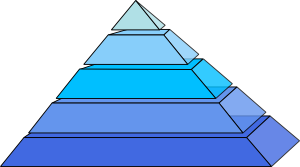
\includegraphics[width=1.1cm]{../Strukturfiler/FIGS/BluePyramid} & \begin{minipage}{\obsl}}{\end{minipage}\\ \end{tabular}\vspace{4mm}\newline}


% = Forudsætning = basis
\newenvironment{basis}{\begin{flushleft} \begin{itshape} }{\end{itshape} \end{flushleft}}


% = Opsummering =
\newenvironment{summary}{\clearpage\pagecolor{sumgul}\section{Opsummering}}{\newpage\pagecolor{white}}











% = Counter
\newcounter{opgavecount}[section]
\setcounter{opgavecount}{0}
\newcounter{spgcount}[opgavecount]
\setcounter{spgcount}{0}
\renewcommand{\thespgcount}{\alph{spgcount})}



% = EXERCISE = (DIVIDER)

\newcommand{\exercisebegin}[1][]{\bigskip\needspace{3\baselineskip}\refstepcounter{opgavecount}\titlegraphic{mingroen}\textcolor{mingroen}{\th{Opgave \theopgavecount \hspace*{1cm} #1}}\medskip\par}

% = QUIZEXERCISE = (DIVIDER)

\newcommand{\quizexercisebegin}[1][]{\bigskip\needspace{3\baselineskip}\refstepcounter{opgavecount}\titlegraphic{mingroen}\textcolor{mingroen}{\th{Quiz-Opgave \theopgavecount \hspace*{1cm} #1}}\medskip\par}

% = QUESTION =

\newenvironment{question}{\refstepcounter{spgcount}\begin{itemize}\item[\thespgcount]}{\end{itemize}\hspace*{\fill}}

% = VINK =

\newenvironment{vink}{\begin{tabular}{m{.9cm}<{\hspace*{2mm}}@{}|m{\obsl}@{}}\hspace*{-4pt}\raggedleft
\includegraphics[width=.9cm]{../Strukturfiler/FIGS/Think} & \begin{minipage}{\obsl}}{\end{minipage}\\ \end{tabular}\medskip\\}
	
% = FACIT =

\newenvironment{facit}{\begin{tabular}{m{.9cm}<{\hspace*{2mm}}@{}|m{\obsl}@{}}\hspace*{-4pt}\raggedleft
\includegraphics[width=.9cm]{../Strukturfiler/FIGS/Check} & \begin{minipage}{\obsl}}{\end{minipage}\\ \end{tabular}\medskip\\}








\newcommand{\afsnit}[1]{\bigskip\th{\titlegraphic{mingroen}\textcolor{mingroen}{#1}} \\ \rule[7pt]{.4\textwidth}{1pt} \vspace*{-2.5mm}\par}

% (DIVIDER):
\newcommand{\ugedagdatotitel}[4]{\pagebreak[4]\section{Semesteruge #1 -- #2 Dag \hspace*{1mm} (#3)} \vspace*{-4mm} \rule[5pt]{\textwidth}{1pt}\vspace*{-2.5mm} \begin{center}\large{\th{#4}}\end{center} \fancyhead[C]{\th{Semesteruge #1}}}

\newenvironment{skema}[1]{\definecolor{shadecolor}{rgb}{0.96,.98, 1.0} \setlength{\FrameSep}{6pt} \renewcommand{\FrameHeightAdjust}{10pt} \vspace*{-4pt}\begin{shaded} \begin{tabular}{#1}}{\end{tabular} \end{shaded} \vspace*{-7pt}}


% ========================

% MAKROER

%\newenvironment{matr}[1][]{\hspace*{-.8mm}\left[\hspace*{-1mm}\begin{array}{#1}}{\end{array}\hspace*{-1mm}\right]\hspace*{-.8mm}}
\newcommand{\bevisslut}{\begin{scriptsize} \begin{flushright} $ \blacksquare $ \end{flushright} \end{scriptsize}}

\newcommand{\tref}[2]{\hyperref[#1]{#2 \ref*{#1}}}
\newcommand{\thref}[2]{\hyperref[#1]{#2}}

\newcommand{\refA}[1]{\colorbox{yellow}{\ref{#1}}}
\newcommand{\hrefA}[2]{\colorbox{yellow}{\href{#1}{#2}}}
\newcommand{\trefA}[2]{\colorbox{yellow}{\hyperref[#1]{#2 \ref*{#1}}}}
\newcommand{\threfA}[2]{\colorbox{yellow}{\hyperref[#1]{#2}}}

\newenvironment{matr}[1]{\hspace*{-.8mm}\begin{bmatrix}\hspace*{-1mm}\begin{array}{#1}}{\end{array}\hspace*{-1mm}\end{bmatrix}\hspace*{-.8mm}}
\newcommand{\transp}{\hspace*{-.6mm}^{\top}}

\newcommand{\maengde}[2]{\left\lbrace \hspace*{-1mm} \begin{array}{c|c} #1 & #2 \end{array} \hspace*{-1mm} \right\rbrace}

\newenvironment{eqnalign}[1]{\setlength{\arraycolsep}{1.3pt}\begin{equation}\begin{array}{#1}}{\end{array}\end{equation}\par}
\newcommand{\eqnl}{\setlength{\arraycolsep}{1.3pt}}

\newcommand{\matind}[3]{{_\mathrm{#1}\mathbf{#2}_\mathrm{#3}}}
\newcommand{\vekind}[2]{{_\mathrm{#1}\mathbf{#2}}}
\newcommand{\jac}[2]{{\mathrm{Jacobi}_\mathbf{#1} (#2)}}
\newcommand{\diver}[2]{{\mathrm{div}\mathbf{#1} (#2)}}
\newcommand{\rot}[1]{{\mathbf{rot}\mathbf{(#1)}}}

\newcommand{\am}{\mathrm{am}}
\newcommand{\gm}{\mathrm{gm}}
\newcommand{\E}{\mathrm{E}}
\newcommand{\Span}{\mathrm{span}}
\newcommand{\mU}{\mathbf{U}}

\newcommand{\ms}{\medskip\\}
\newcommand{\bs}{\bigskip\\}

\newcommand{\mA}{\mathbf{A}}
\newcommand{\mB}{\mathbf{B}}
\newcommand{\mC}{\mathbf{C}}
\newcommand{\mD}{\mathbf{D}}
\newcommand{\mE}{\mathbf{E}}
\newcommand{\mF}{\mathbf{F}}
\newcommand{\mK}{\mathbf{K}}
\newcommand{\mI}{\mathbf{I}}
\newcommand{\mM}{\mathbf{M}}
\newcommand{\mN}{\mathbf{N}}
\newcommand{\mQ}{\mathbf{Q}}
\newcommand{\mT}{\mathbf{T}}
\newcommand{\mV}{\mathbf{V}}
\newcommand{\mW}{\mathbf{W}}
\newcommand{\mX}{\mathbf{X}}
\newcommand{\ma}{\mathbf{a}}
\newcommand{\mb}{\mathbf{b}}
\newcommand{\mc}{\mathbf{c}}
\newcommand{\md}{\mathbf{d}}
\newcommand{\me}{\mathbf{e}}
\newcommand{\mn}{\mathbf{n}}
\newcommand{\mr}{\mathbf{r}}
\newcommand{\mv}{\mathbf{v}}
\newcommand{\mw}{\mathbf{w}}
\newcommand{\mx}{\mathbf{x}}
\newcommand{\mxb}{\mathbf{x_{bet}}}
\newcommand{\my}{\mathbf{y}}
\newcommand{\mz}{\mathbf{z}}
\newcommand{\reel}{\mathbb{R}}
\newcommand{\mL}{\bm{\Lambda}} %Lambda-matrix
\newcommand{\mnul}{\bm{0}}
\newcommand{\trap}[1]{\mathrm{trap}(#1)}
\newcommand{\Det}{\operatorname{Det}}
\newcommand{\adj}{\operatorname{adj}}
\newcommand{\Ar}{\operatorname{Areal}}
\newcommand{\Vol}{\operatorname{Vol}}
\newcommand{\Rum}{\operatorname{Rum}}
\newcommand{\diag}{\operatorname{\bf{diag}}}
\newcommand{\bidiag}{\operatorname{\bf{bidiag}}}
\newcommand{\spanVec}[1]{\mathrm{span}\{#1\}}
\newcommand{\Div}{\operatorname{Div}}
\newcommand{\Rot}{\operatorname{\mathbf{Rot}}}

\newcommand{\Jac}{\operatorname{Jacobi}}
\newcommand{\Tan}{\operatorname{Tan}}
\newcommand{\Ort}{\operatorname{Ort}}
\newcommand{\Flux}{\operatorname{Flux}}
\newcommand{\Cmass}{\operatorname{Cm}}
\newcommand{\Imom}{\operatorname{Im}}
\newcommand{\Pmom}{\operatorname{Pm}}
\newcommand{\IS}{\operatorname{I}}
\newcommand{\IIS}{\operatorname{II}}
\newcommand{\IIIS}{\operatorname{III}}
\newcommand{\Le}{\operatorname{L}}
\newcommand{\app}{\operatorname{app}}
\newcommand{\M}{\operatorname{M}}
\newcommand{\re}{\mathrm{Re}}
\newcommand{\im}{\mathrm{Im}}

\newcommand{\compl}{\mathbb{C}} %de komplekse tal
\newcommand{\e}{\mathrm{e}} %eksponentialfunktionen. lodret 'e', og altså ikke kursiv ligesom andre bogstaver.





% Medialink: SCREEN: (QRcode) + thumbnail image + link på kodenummer (til qr.dtu.dk)
\newcommand{\onlinemedia}[3]{
	\begin{wrapfigure}{r}{3.2cm} 
		\vspace{-30pt} 
		\vspace{#1pt} 
		\begin{flushright} 
			\includegraphics[width=3cm]{qr/#2.png} 
			\tiny 
			\href{http://qr.dtu.dk/#2}{#2: #3}
			\normalsize  
		\end{flushright} 
		\vspace{-10pt} 
	\end{wrapfigure}
}
\newcommand{\onlinemediathumb}[3]{
	\begin{wrapfigure}{r}{3.2cm} 
		\vspace{-30pt} 
		\vspace{#1pt} 
		\begin{flushright} 
			\includegraphics[width=3cm]{qr/#2.png} 
			\includegraphics[width=3cm]{qr/#2_thumb.png} 
			\tiny 
			\href{http://qr.dtu.dk/#2}{#2: #3}
			\normalsize  
		\end{flushright} 
		\vspace{-10pt} 
	\end{wrapfigure}
}



% Index:
\usepackage{makeidx}
\makeindex
\newcommand\ind[2]{\index{#1}\textbf{\textit{\textcolor{black}{#2}}}}

% ###SERVER_EXCLUDE_BEGIN###
\externaldocument[NUID17-]{../../enoten/TN01-Talrum/Talrum}
\externaldocument[NUID1-]{../../enoten/TN02-Ligningssystemer/TNdriver}
\externaldocument[NUID2-]{../../enoten/TN03-Matricer_og_Matrixalgebra/Matricer_og_matrixalgebra}
\externaldocument[NUID3-]{../../enoten/TN04-Kvadratiske_matricer/TNdriver}
\externaldocument[NUID11-]{../../enoten/TN05-Determinanter/Determinanter}
\externaldocument[NUID12-]{../../enoten/TN06-GeometriskeVektorer/GeometriskeVektorer}
\externaldocument[NUID18-]{../../enoten/TN07-Vektorrum/VektorRum}
\externaldocument[NUID21-]{../../enoten/TN08-LinAfbildninger/LinAfbildninger}
\externaldocument[NUID23-]{../../enoten/TN09-Egenvaerdier_og_egenvektorer/TNdriver}
\externaldocument[NUID24-]{../../enoten/TN10-Diagonalisering_med_egenvektorer/TNdriver}
\externaldocument[NUID10-]{../../enoten/TN11-1.ordens_differentialligninger/TNdriver}
\externaldocument[NUID13-]{../../enoten/TN12-1.ordens_differentialligningssystemer/TNdriver}
\externaldocument[NUID14-]{../../enoten/TN13-2.ordens_differentialligninger/TNdriver}
\externaldocument[NUID27-]{../../enoten/TN14-Elemenataere_funktioner/Elementaere_Funktioner}
\externaldocument[NUID28-]{../../enoten/TN15-Funktioner2Variable/Funktioner_To_Variable}
\externaldocument[NUID29-]{../../enoten/TN16-Gradienter_og_Tangentplaner/Gradienter_og_Tangentplaner}
\externaldocument[NUID32-]{../../enoten/TN17-Taylor_formler/Taylor_Formler}
\externaldocument[NUID33-]{../../enoten/TN18-Taylor_2Var/Taylor_2Var}
\externaldocument[NUID34-]{../../enoten/TN19-SymMat/SymmetriskeMatricer}
\externaldocument[NUID35-]{../../enoten/TN20-KegleSnit/Keglesnit}
\externaldocument[NUID36-]{../../enoten/TN21-Riemann_Integral/Riemann_01}
\externaldocument[NUID37-]{../../enoten/TN22-Plan_Int/Plan_Int_01}
\externaldocument[NUID39-]{../../enoten/TN23-Flade_Int/Flade_Rum_Int_01}
\externaldocument[NUID40-]{../../enoten/TN24-Vektorfelter/Vektorfelter_01}
\externaldocument[NUID41-]{../../enoten/TN25-Flux/Flux_02}
\externaldocument[NUID42-]{../../enoten/TN26-Gauss/Gauss_01}
\externaldocument[NUID128-]{../../enoten/TN27-Stokes/Stokes_01}
\externaldocument[NUID43-]{../../enoten/TN29-KomplekseTal/KomplekseTal}

\externaldocument[NUID6-]{../../E-math-opgaver/Opgaver/opgU123}
\externaldocument[NUID19-]{../../E-math-opgaver/Opgaver/opgU45}
\externaldocument[NUID20-]{../../E-math-opgaver/Opgaver/opgU678}
\externaldocument[NUID25-]{../../E-math-opgaver/Opgaver/opgU910SD}
\externaldocument[NUID31-]{../../E-math-opgaver/OpgaverF11-U123/opgF123}
% \externaldocument[NUID9-]{../../E-math-opgaver/Opgaver/Dagsordner E10}
% ###SERVER_EXCLUDE_END###


% Begin document and set alternative chapter title:
\begin{document}
\renewcommand{\chaptername}{eNote}

\setcounter{chapter}{5} %SÆT DETTE TAL TIL 1 MINDRE END DET AKTUELLE TRANSFERNOTE-NUMMER!!

%%%%%%%%%%%%%%%%%%%%%%%%%%%%%%%%%%%%%%%%%%%%%
%%%%%%%%%%%%%%%%%%%%%%%%%%%%%%%%%%%%%%%%%%%%%
%%% HERFRA SKAL DU SKRIVE ELLER INDSÆTTE %%%%
%%% DEN FIL DU ØNSKER %%%%%%%%%%%%%%%%%%%%%%%
%%%%%%%%%%%%%%%%%%%%%%%%%%%%%%%%%%%%%%%%%%%%%
%%%%%%%%%%%%%%%%%%%%%%%%%%%%%%%%%%%%%%%%%%%%%

\chapter{Geometriske vektorer} \label{tn6}

%%%%%%%%%%%%%%%%%%%%%%%%%%%%%%%%%%%%%%%%%%%%%%%%%%%%%%%%%%
%%%%%%%%%%%%%%%%%%%%%%%%%%%%%%%%%%%%%%%%%%%%%%%%%%%%%%%%%%
%%%%%%%%%%%%%%%%%%%%%%%%%%%%%%%%%%%%%%%%%%%%%%%%%%%%%%%%%%
\begin{basis}
Formålet med denne note er at give en introduktion til geometriske vektorer i planen og rummet, som sigter mod at introducere en række af de metoder der gør sig gældende i den generelle vektorrumsteori. Nøglebegreberne er her \textit{lineær uafhængighed} og \textit{lineær afhængighed}, samt \textit{basis} og \textit{koordinater}. Noten forudsætter kendskab til elementær plan- og rumgeometri, til lineære ligningssystemer som beskrevet i \tref{NUID1-tn2}{eNote} og til matrixalgebra som beskrevet i \tref{NUID2-tn3}{eNote}.
\end{basis}

Ved en \ind{geometrisk vektor}{geometrisk vektor} i planen eller rummet forstås et sammenhørende par bestående af en \textit{længde} og en \textit{retning}. Geometriske vektorer skrives med små fede bogstaver, for eksempel $\mathbf{v}$. En vektor kan repræsenteres af et \ind{orienteret linestykke}{orienteret linjestykke} med et givet begyndelsespunkt og endepunkt. Hvis vektoren $\mathbf{v}$ er repræsenteret af det orienterede linjestykke fra begyndelsespunktet $A$ til endepunktet $B$, benytter vi skrivemåden $\mathbf{v}=\stackrel{\rightarrow}{AB}$. Alle orienterede linjestykker som har samme længde og retning som det orienterede linjestykke fra $A$ til $B$, er også repræsentanter for
$\textbf{v}$.
\begin{example}[Parallelforskydninger ved hjælp af vektorer]
Geometriske vektorer kan benyttes til at angive \ind{parallelforskydning}{parallelforskydninger} i planen eller rummet. På figur 6.1 er linjestykket $CD$ fremkommet af linjestykket $AB$ ved at alle punkterne på $AB$ er blevet forskudt med vektoren $\mathbf{u}$. På samme måde er linjestykket $EF$ fremkommet af $AB$ ved parallelforskydning med vektoren $\mathbf{v}$.
%%%%%%%%%%%%%%%%%%%%%%%%%%%%%%%%%%%%%%%%%%%%%%%
%Om figurer: trim= klippes fra: øst syd vest nord, clip=du ser ikke det der er klippet fra, uden for feltet.
%%%%%%%%%%%%%%%%%%%%%%%%%%%%%%%%%%%%%%%%%%%%%%%

\begin{center}
	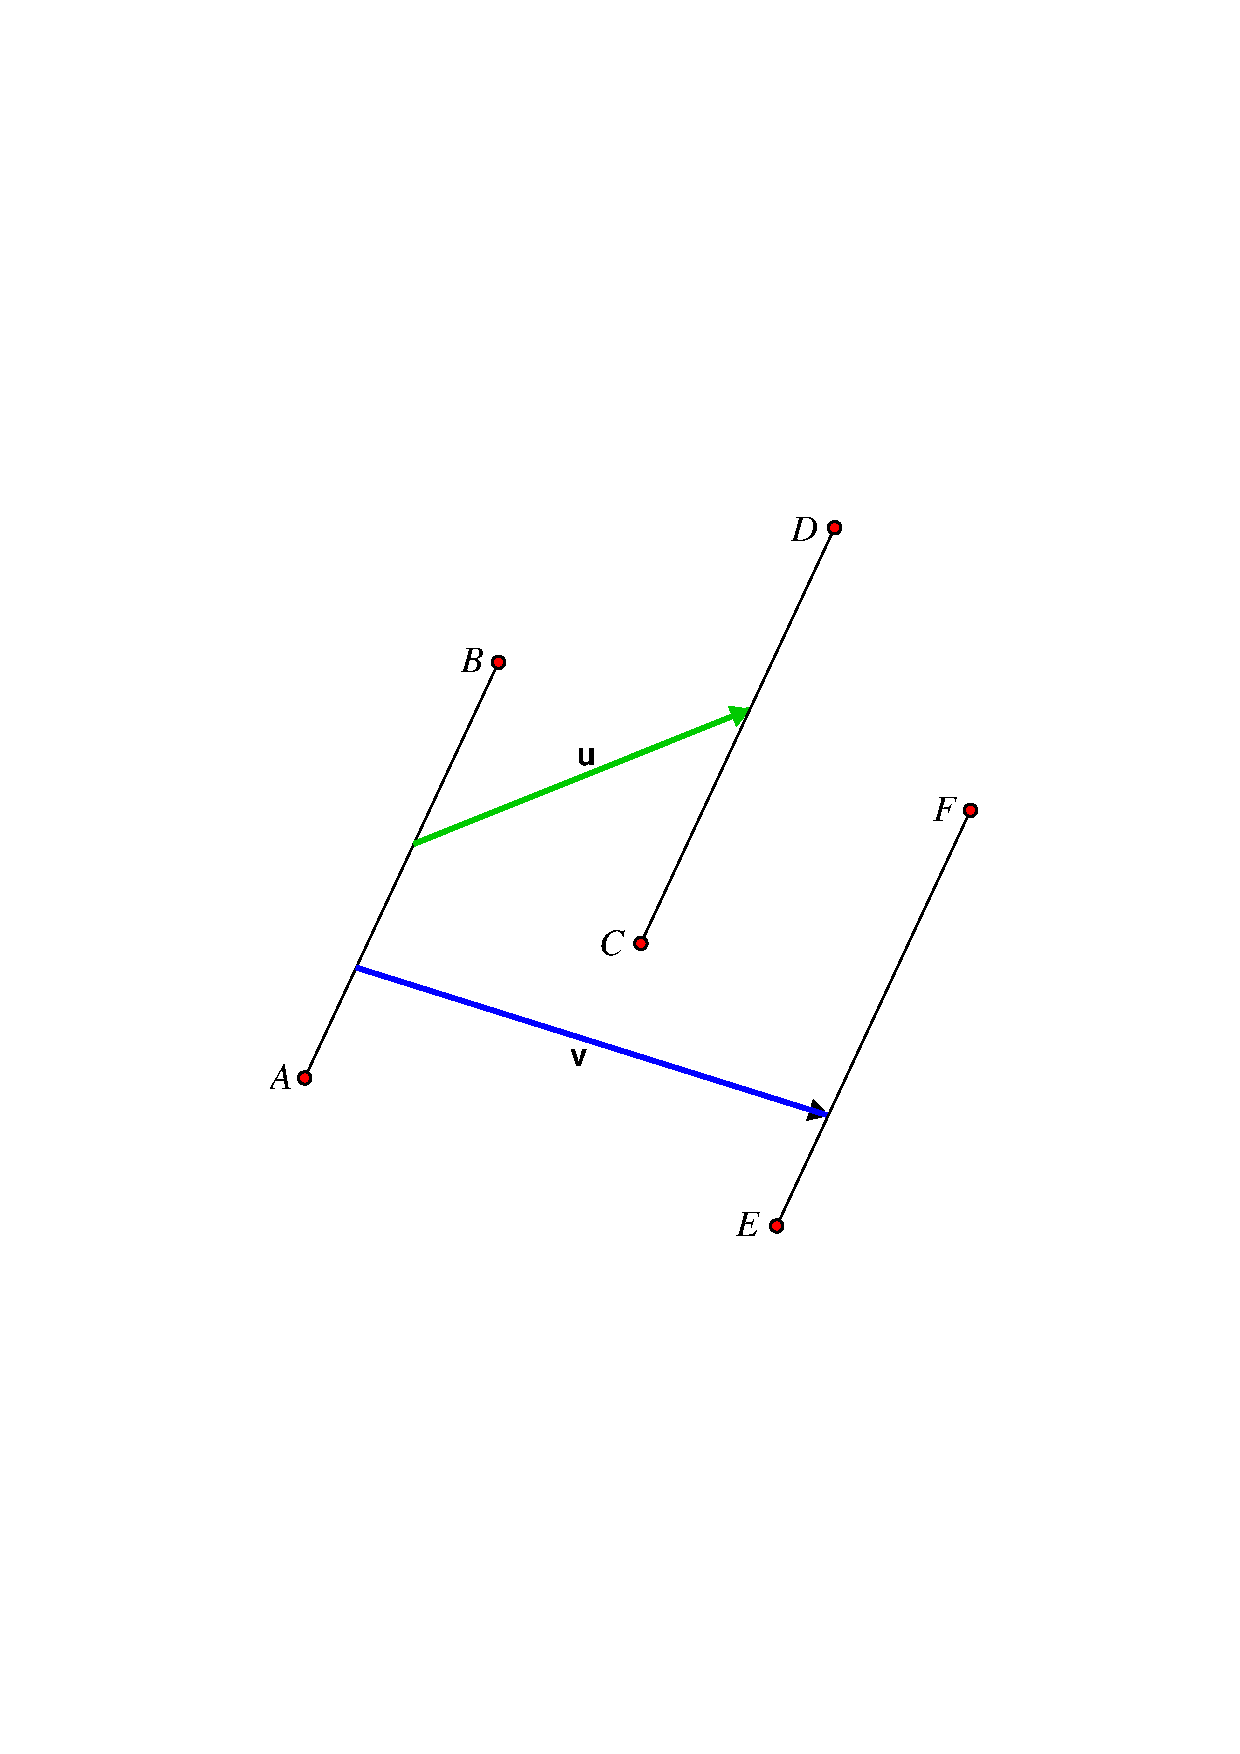
\includegraphics[trim=4.2cm 8.5cm 4cm 8.7cm,width=0.44\textwidth,clip]{geometer/vektor1.pdf}\\

Figur 6.1: Parallelforskydning ved hjælp af vektorer				
\end{center}
Der gælder at $\stackrel{\rightarrow}{AB}\,=\,\stackrel{\rightarrow}{CD}\,=\,\stackrel{\rightarrow}{EF}$, men bemærk for eksempel også at 
$\stackrel{\rightarrow}{AB}\,\neq\,\stackrel{\rightarrow}{FE}$.
\end{example}

I det følgende forudsætter vi at der er valgt et \textit{enhedslinjestykke}, det vil sige et linjestykke der tillægges længden 1. Ved $|\mathbf v|$ forstås længden af vektoren $\mathbf v$ set i forhold til længden af enhedslinjestykket, det vil sige et reelt tal. Alle vektorer som har samme længde som enhedslinjestykket kaldes \ind{enhedsvektor}{enhedsvektorer}.\\

Af praktiske grunde indføres en særlig vektor som har længden $0\,$ og som ikke tillægges en retning. Den kaldes \ind{nul-vektoren}{nul-vektoren} og skrives \textbf{0}. For ethvert punkt $A$ sætter vi $\stackrel{\rightarrow}{AA}\,=\,$\textbf{0}. En vektor, som ikke nulvektoren, kaldes for en \textit{egentlig} vektor.\\

For enhver egentlig vektor $\mv$ defineres den \textit{modsatte vektor} $-\mv$ som den vektor der har samme længde som $\mv\,$, men modsat retning. Hvis $\mv\,=\,\stackrel{\rightarrow}{AB},$ gælder dermed at  $\stackrel{\rightarrow}{BA}\,=\,-\mv\,.$ For nulvektoren sættes $-\mnul\,=\,\mnul\,$.\\   

Det er ofte praktisk at benytte et fælles begyndelsespunkt når forskellige vektorer skal repræsenteres af orienterede linjestykker. Man vælger derfor et fast punkt $O$, kaldet \textit{origo}, og betragter de repræsentanter for vektorerne som har $O$ som sit begyndelsespunkt. Vektorer som er repræsenteret på denne måde kaldes \ind{stedvektor}{stedvektorer}, fordi der til enhver given vektor $\mathbf{v}$ hører ét unikt punkt (eller sted) $P$ der opfylder at 
$\mathbf{v}=\stackrel{\rightarrow}{OP}$. Tilsvarende hører der til ethvert punkt $Q$ én unik vektor $\mathbf u$ således at $\stackrel{\rightarrow}{OQ}\,=\,\mathbf{u}$.\\

Ved \textit{vinklen mellem to egentlige vektorer i planen} forstår man den entydigt bestemte vinkel mellem deres repræsentanter udgående fra $O\,$, som ligger i intervallet $\left[\,0;\pi\right]\,$. Hvis en vektor $\mv$ i planen drejes vinklen $\,\pi /2\,$ mod uret, fremkommer en ny vektor der kaldes $\mv$'s \textit{tværvektor}, den betegnes $\widehat{\mathbf{v}}$.\\

Ved \textit{vinklen mellem to egentlige vektorer i rummet} forstås vinklen  mellem deres repræsentanter udgående fra $O$ i den plan som indeholder repræsentanterne.\\

Det giver god og brugbar mening ``at lægge vektorer sammen'', idet man både tager højde for vektorernes længde og deres retning. Vi kan derfor i det følgende indføre nogle regneoperationer for geometriske vektorer. I første omgang drejer det sig om de to \textit{lineære regneoperationer}, addition af vektorer og multiplikation af vektor med en skalar (et reelt tal). Senere skal vi se på tre forskellige måder at multiplicere vektorer med hinanden på, nemlig \textit{prikprodukt}, og for rumvektorer \textit{krydsprodukt} og \textit{rumprodukt}.
%%%%%%%%%%%%%%%%%%%%%%%%%%%%%%%%%%%%%%%%%%%%%%%%%%%%%%%%%%
%%%%%%%%%%%%%%%%%%%%%%%%%%%%%%%%%%%%%%%%%%%%%%%%%%%%%%%%%%
%%%%%%%%%%%%%%%%%%%%%%%%%%%%%%%%%%%%%%%%%%%%%%%%%%%%%%%%%%
\section{Addition og multiplikation med skalar}
\vspace{-0.5cm}
\begin{definition}[Addition]\label{addition}
Der er givet to vektorer i planen eller rummet, $\mathbf u$ og $\mathbf v$. Summen $\mathbf u +\mathbf v$ fastlægges ved følgende metode:
\vspace{-0.3cm}
\begin{itemize}
\item
Vi vælger origo $O$ og afsætter stedvektorerne $\mathbf{u}=\stackrel{\rightarrow}{OQ}$ og
$\mathbf{v}=\stackrel{\rightarrow}{OR}$.
\item
Ved parallelforskydning af linjestykket $OR$ med $\mathbf u$ fremkommer linjestykket $QP$. 
\item
 $\stackrel{\rightarrow}{OP}$ er da stedvektor for summen af $\mathbf u$ og $\mathbf v$, kort sagt $\mathbf u +  \mathbf v\,=\,\stackrel{\rightarrow}{OP}$.
\end{itemize}
\begin{center}
		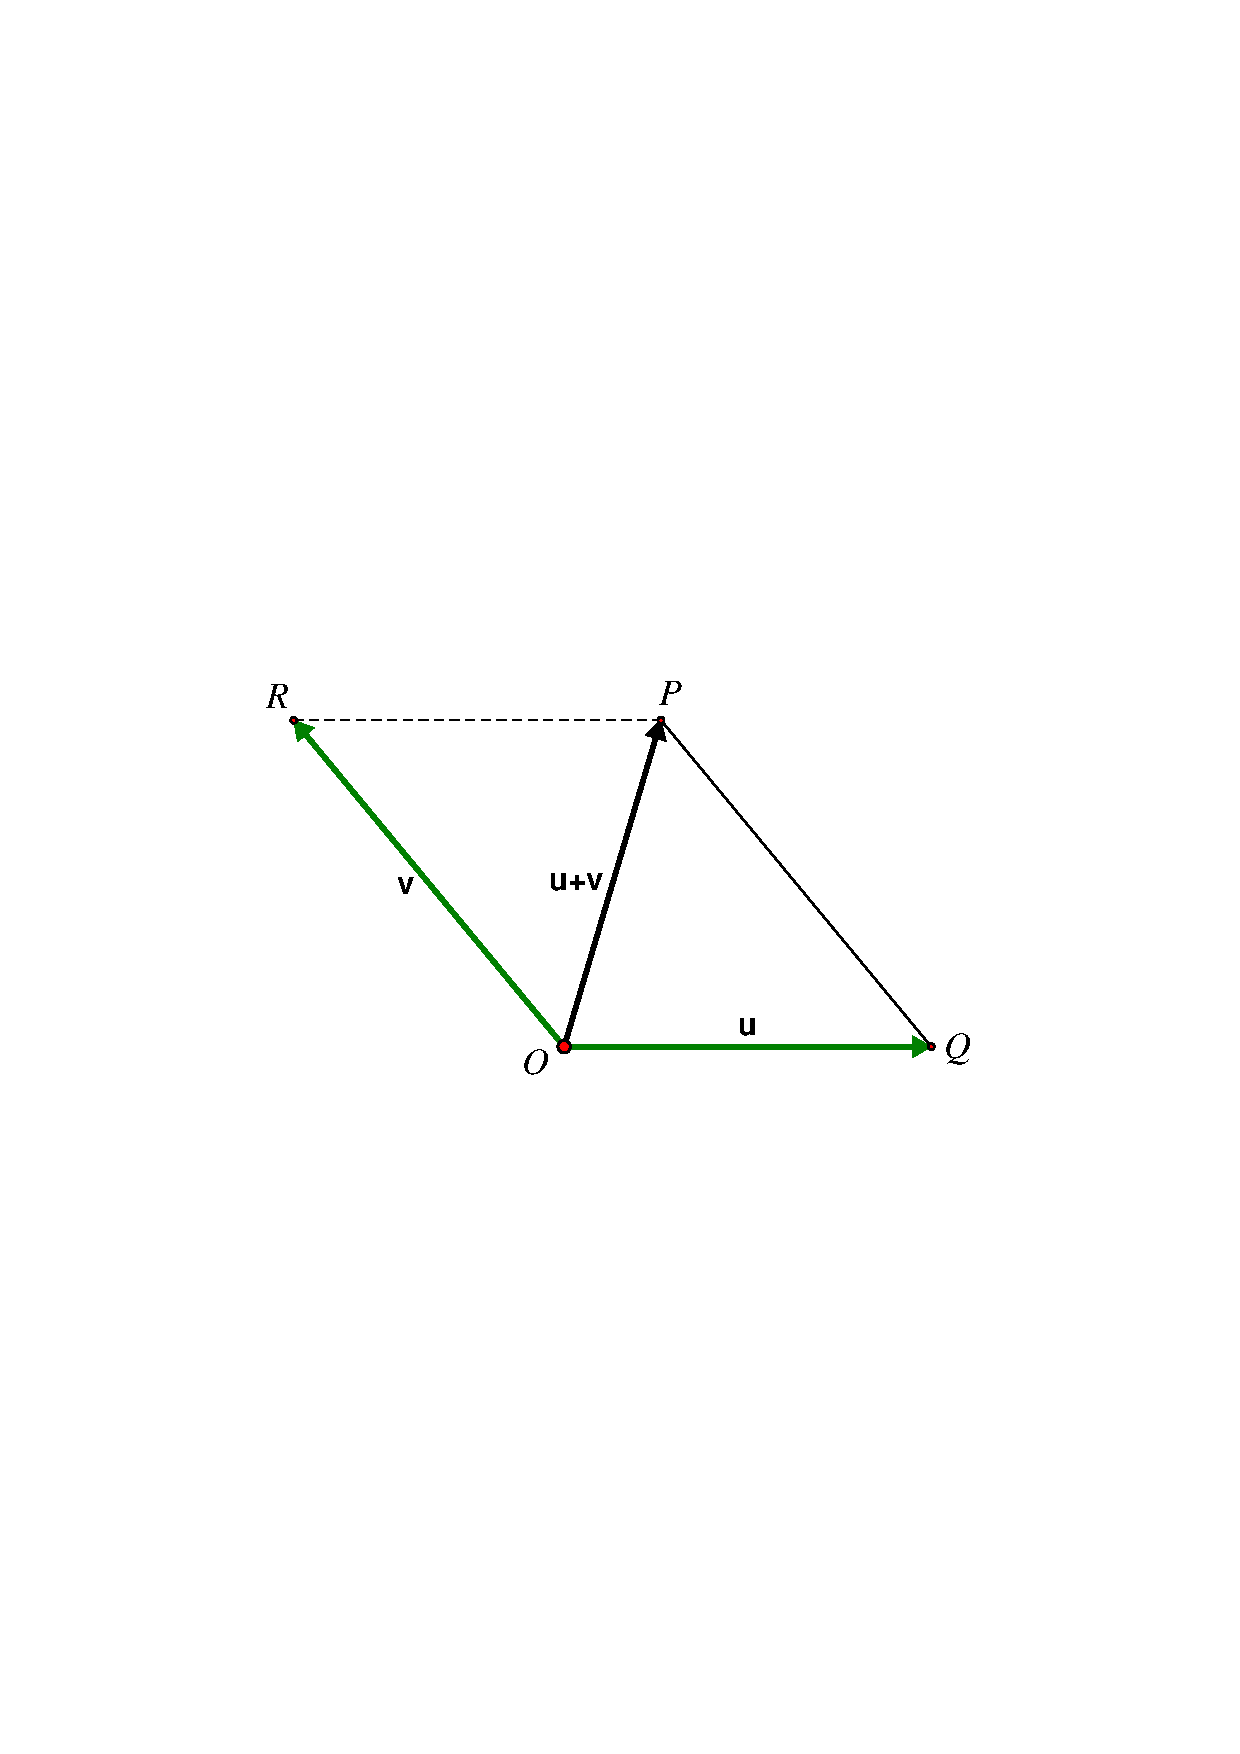
\includegraphics[trim=4cm 11.5cm 4cm 11.5cm,width=0.50\textwidth,clip]{geometer/vektor2.pdf}
%Figur 6.2: Addition af to vektorer				
\end{center}
\end{definition}
\begin{info}
I fysik taler man om ''kræfternes parallelogram'': Hvis objektet $O$ er påvirket af kræfterne $\mathbf u$ og $\mathbf v$, kan den \textit{resulterende kraft} bestemmes som sumvektoren $\mathbf u+ \mathbf v$, hvis retning angiver den resulterende krafts retning, og hvis længde angiver kraftens størrelse. Hvis specielt $\mathbf u$ og $\mathbf v$ har samme længde, men modsat retning, er den resulterende kraft lig med $\mnul$-vektoren.  
\end{info} 

Vi indfører herefter multiplikation af vektor med skalar:\medskip \\
\begin{definition}[Multiplikation med skalar]\label{multiplikation}
Der er givet en vektor $\mathbf v$ i planen eller rummet og en skalar $k$. Hvis $\mv =\mnul$, sætter vi $k\mathbf v=\mathbf v k=\mnul$. I modsat forstås der ved produktet $k\mathbf v$ følgende:
\begin{itemize}
\item
Hvis $k>0$, så er $k\mathbf v=\mathbf v k$ den vektor som har samme retning som $\mathbf v$, og som er $k$ gange så lang som $\mathbf v$.
\item
Hvis $k=0$, så er $k\mathbf v=\,$\textbf{0}.
\item
Hvis $k<0$, så er $k\mathbf v=\mathbf v k$ den vektor som har den \textit{modsatte retning} af $\mathbf v$, og som er $-k=|\,k\,|$ gange så lang som $\mathbf v$.
\end{itemize}
\end{definition}

\begin{example}[Multiplikation med skalar]
En given vektor $\mv$ ganges med henholdsvis $-1$ og $2\,:$ 
\begin{center}
		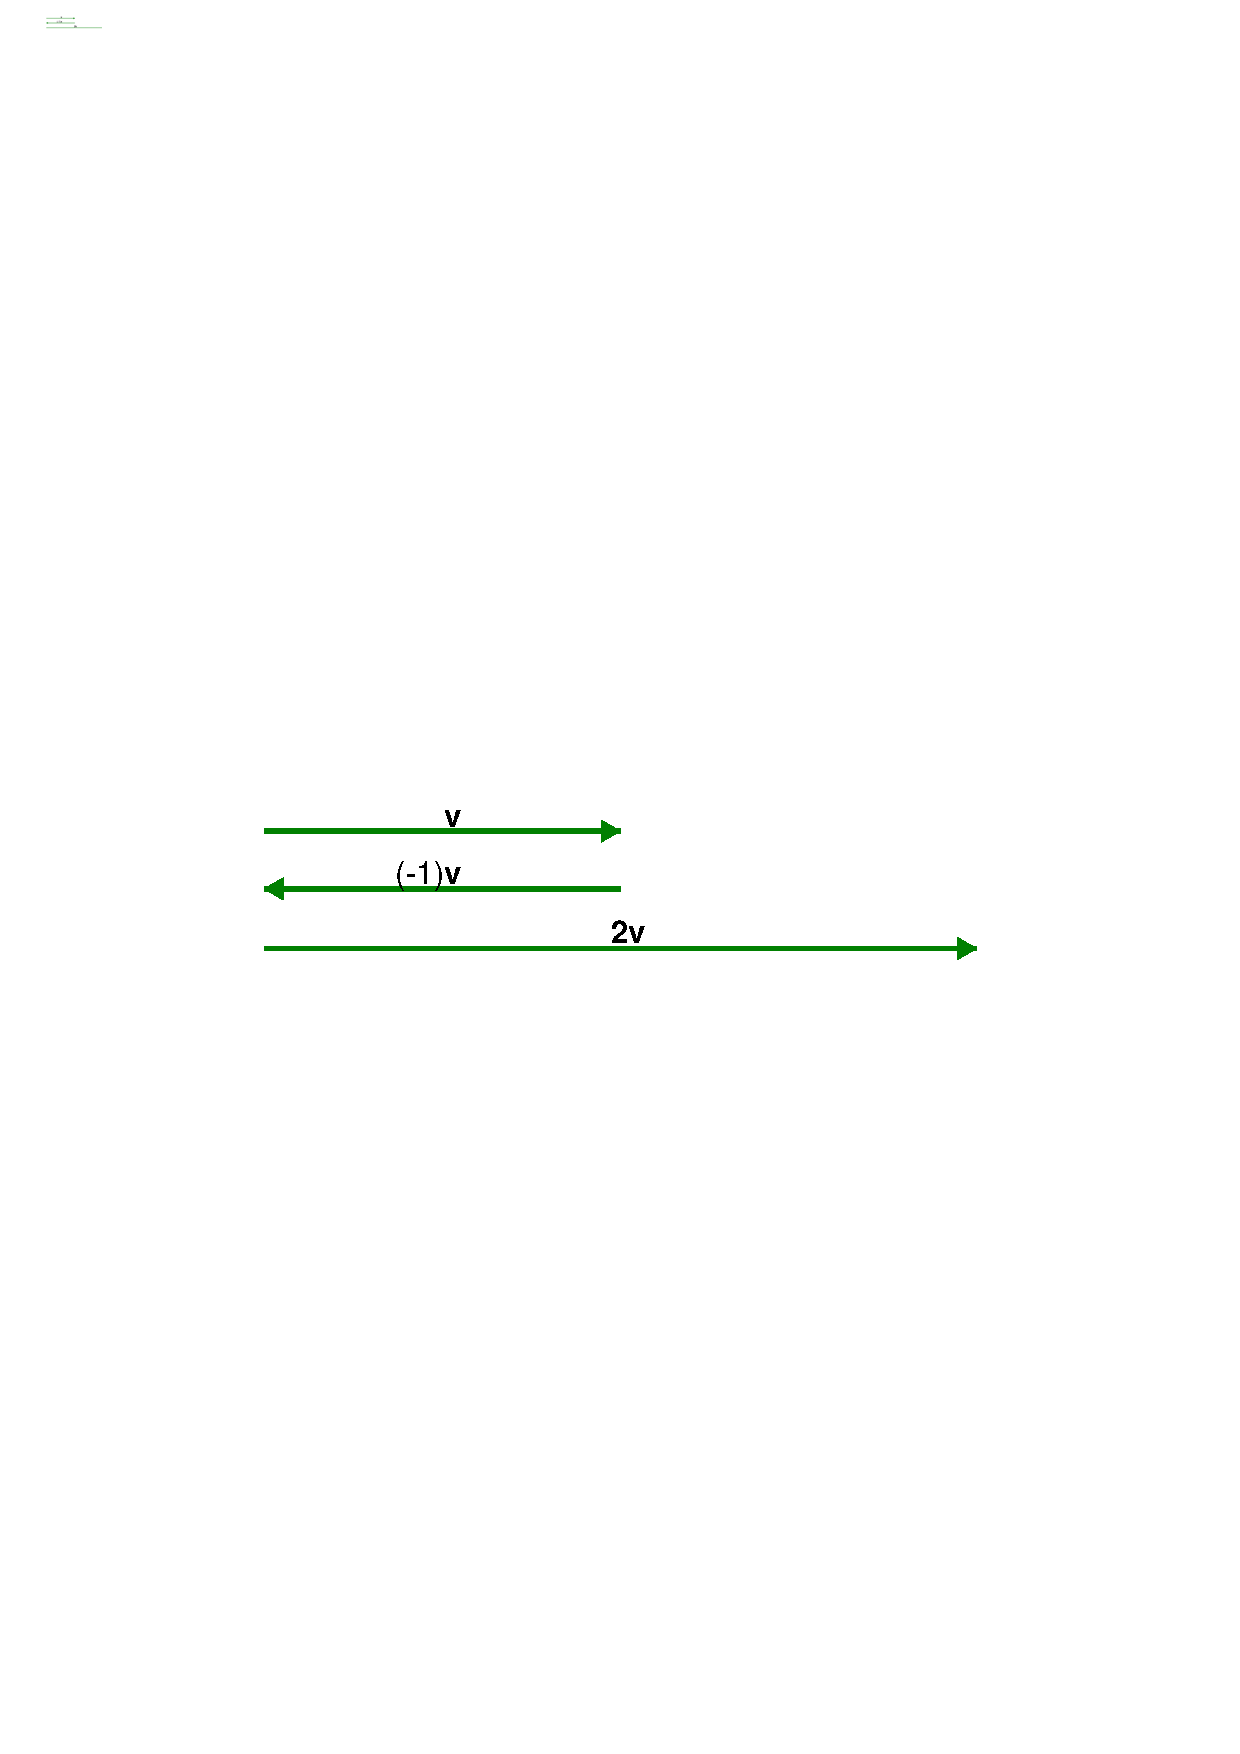
\includegraphics[trim=4cm 13.5cm 4cm 13.5cm,width=0.50\textwidth,clip]{geometer/vektor3.pdf}
\\Figur 6.2: Multiplikation af en vektor med -1 og 2		
\end{center}
\end{example}

\begin{aha}
Det følger umiddelbart af defintion \ref{multiplikation} at multiplikation af en vektor med $-1$ giver vektorens modsatte vektor, kort sagt $$(-1)\mathbf u=-\mathbf u\,.$$ I forlængelse her af bruger vi skrivemåder som $$ (-5)\mv=-(5\mv)=-5\mv\,.$$ 
\end{aha}

\begin{aha}
Af defintion \ref{multiplikation} følger umiddelbart \textit{nulreglen} for geometriske vektorer:
$$k\mv=\mnul\,\Leftrightarrow\,k=0\,\,\,\mathrm{eller}\,\,\,\mv=\mnul\,.$$
\end{aha}

I det følgende eksempel vises at multiplikation af en vilkårlig vektor en en vilkårlig skalar kan udføres ved ren passer/lineal konstruktion. %alternativt kræver det blot multiplikation af to vilkårlige reelle tal

\begin{example}[Geometrisk multiplikation]
Der er givet en vektor $\mathbf a$ og et linjestykke med længden $k$, vi ønsker at konstruere vektoren $k\mathbf a$. 
\begin{center}
		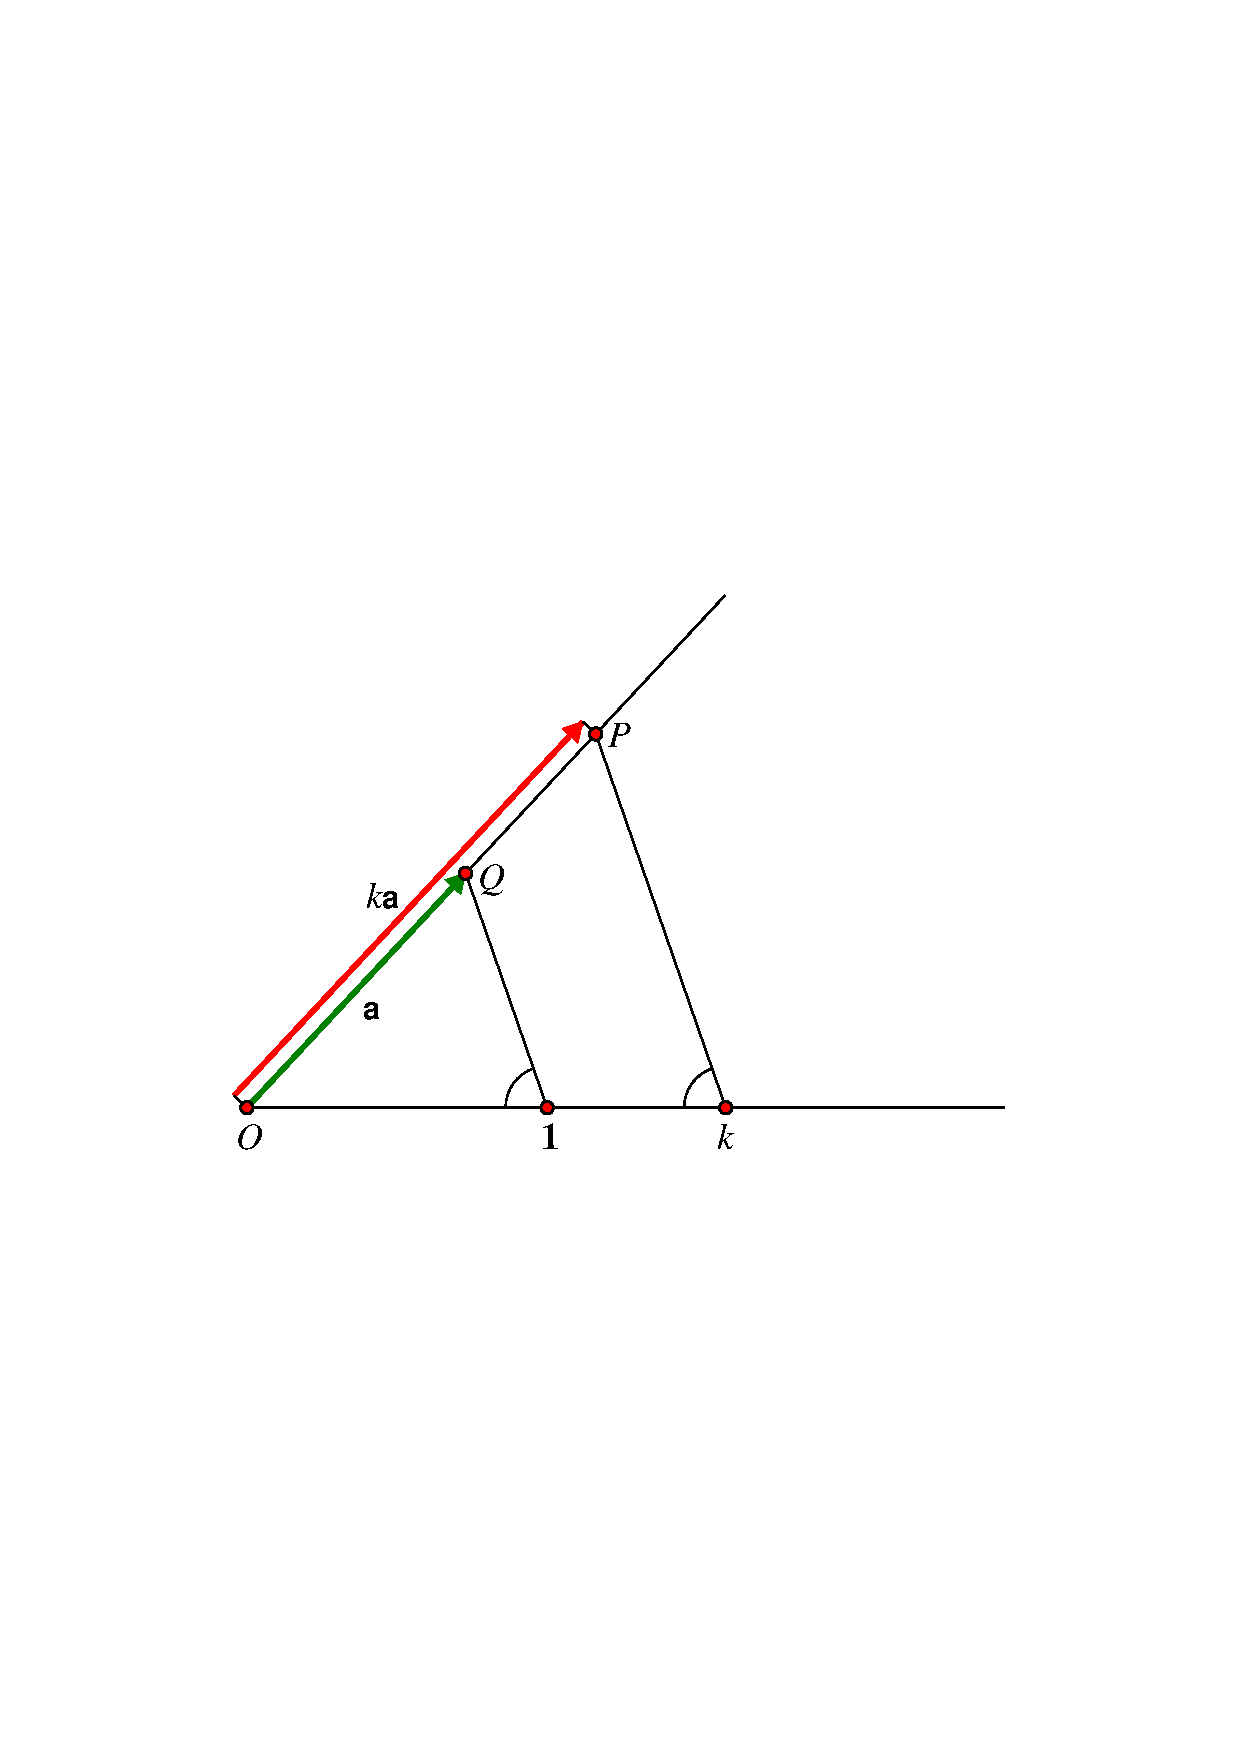
\includegraphics[trim=4cm 10cm 6cm 10.5cm,width=0.45\textwidth,clip]{geometer/vektor4.pdf}\\Figur 6.3: Multiplikation af vektor med vilkårlig skalar				
\end{center}
Først afsættes $\stackrel{\rightarrow}{OQ}=\mathbf a$. Derefter indlægges der med $O$ som begyndelsespunkt en målelinje (lineal) som ikke er parallel med $\mathbf a$, og hvor tallene 1 og $k$ er afsat. Trekanten $OkP$ tegnes så den er ensvinklet med trekanten $O1Q$. Da de to trekanter er ensvinklede, må der gælde at $k\mathbf a=\stackrel{\rightarrow}{OP}$.
\end{example}
\begin{exercise}
Der er på et stykke papir givet to parallelle vektorer $\mathbf a$ og $\mathbf b$ samt en målelinje. Find ved konstruktion et linjestykke som har længden $k$, og som opfylder at $\mathbf b=k\mathbf a$. 
\end{exercise}
\begin{exercise}
Der er på papiret givet en egentlig vektoren $\mathbf v$, og der er givet en målelinje (lineal). Tegn vektoren $\frac 1 {|\mv|}\,\mv$. 
\end{exercise}
\textit{Parameterfremstillinger for rette linjer i planen eller rummet} opstilles ved hjælp af egentlige vektorer. Nedenfor giver vi først et eksempel på en linje der går gennem origo, dernæst et eksempel på en linje der ikke gør det.

\begin{example}[Parameterfremstilling for ret linje]
Der er givet en ret linje $\,l\,$ som går gennem origo, vi ønsker at beskrive punkterne på linjen ved hjælp af en \ind{parameterfremstilling}{parameterfremstilling}:
\begin{center}
		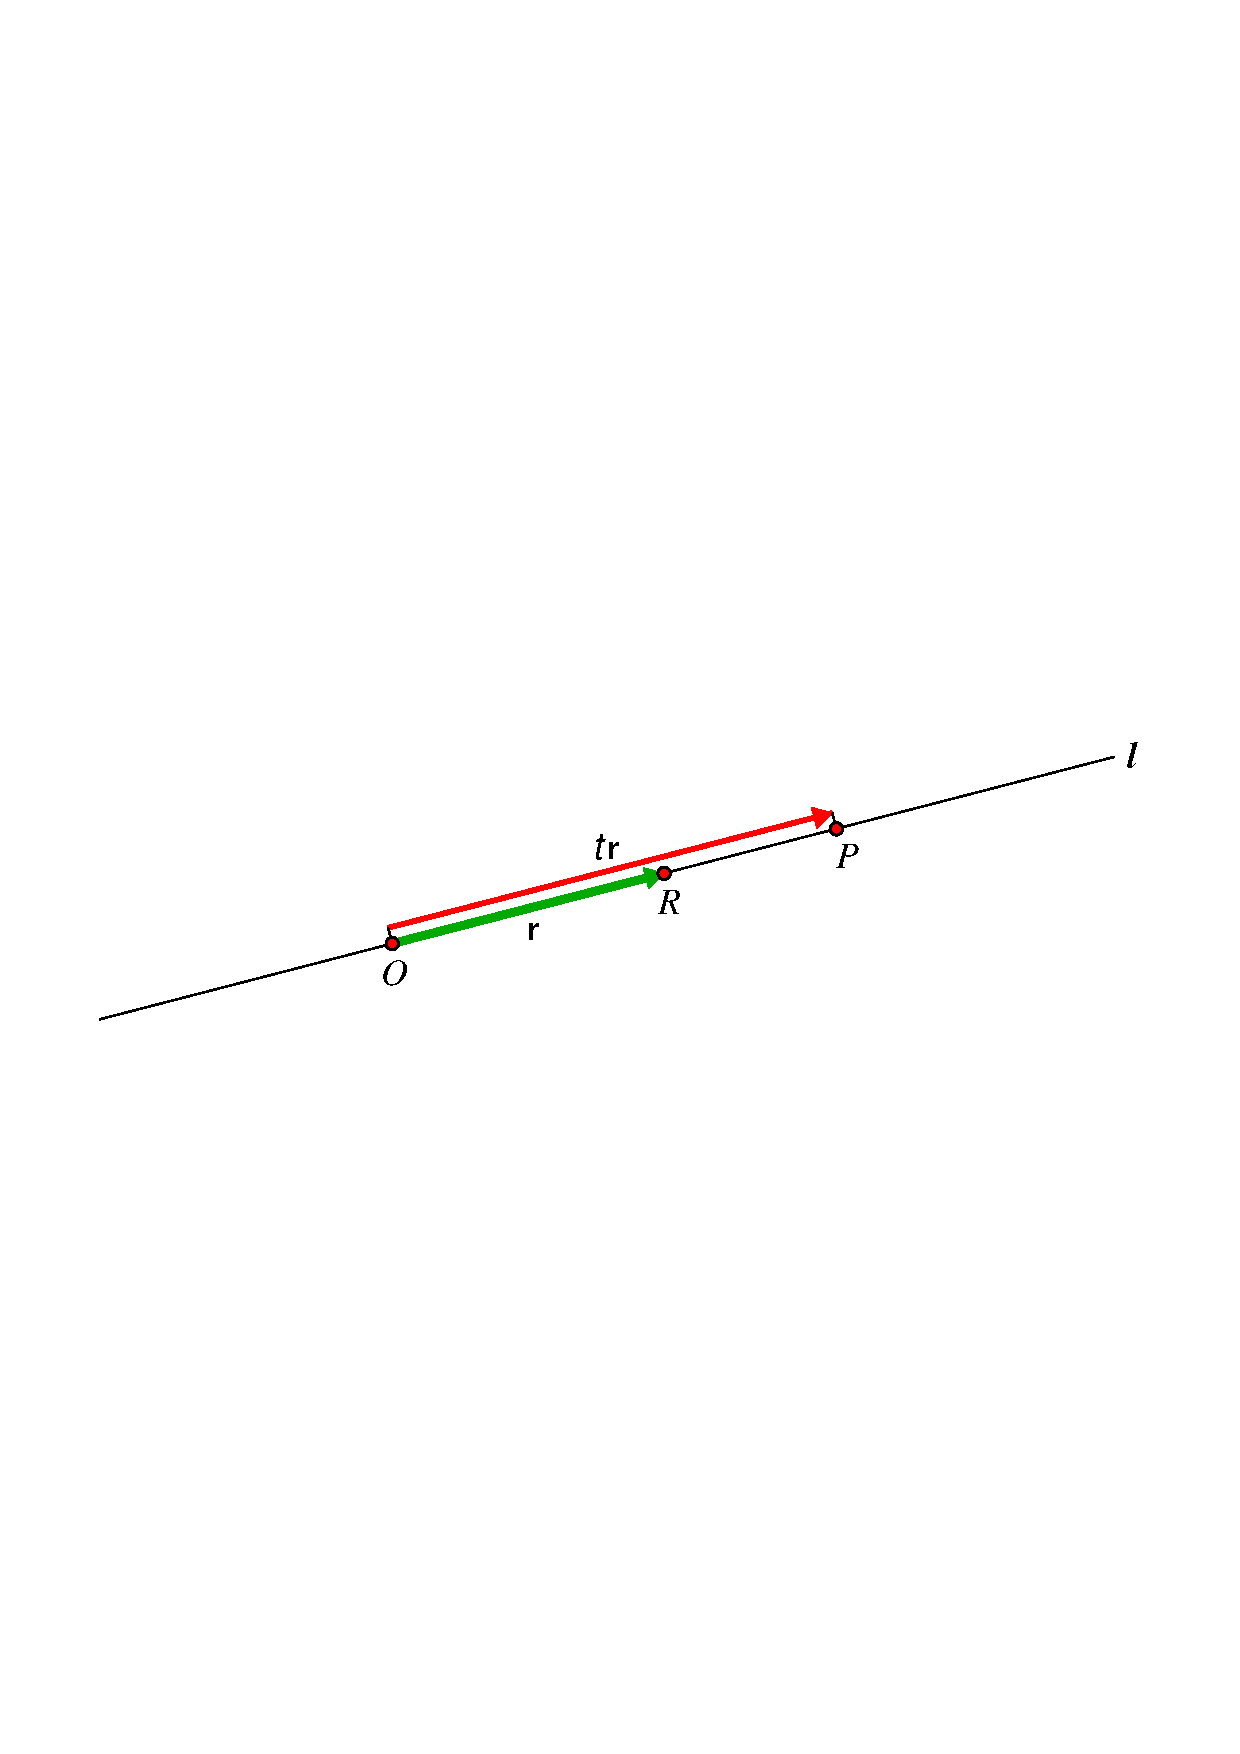
\includegraphics[trim=1cm 12cm 1cm 12cm, width=0.60\textwidth,clip]{geometer/vektor7b.pdf}
		\\Figur 6.4: Parameterfrestilling for linje gennem origo		
\end{center}
Der vælges et punkt $R$ på $l$ som ikke er det samme som origo. Vektoren $\mathbf r=\stackrel{\rightarrow}{OR}$ kaldes en  \ind{retningsvektor}{retningsvektor} for $\,l\,$. Til ethvert punkt $P$ på $\,l\,$ svarer der netop et reelt tal $t$ der opfylder at $\stackrel{\rightarrow}{OP}=t\mathbf r$. Omvendt svarer der til ethvert tal $t$ netop et punkt $P$ på $l$ så $\stackrel{\rightarrow}{OP}=t\mathbf r\,$. Når $t$ \textit{gennemløber} de reelle tal fra -$\infty$ til +$\infty$, vil $P$ \textit{gennemløbe} hele $\,l\,$ i den retning som er bestemt ved $\mathbf r$. Man siger at 
$$\{\,P\,|\,\stackrel{\rightarrow}{OP}=t\mathbf r\,\,\mathrm{hvor}\,\,t \in \mathbb R\,\}$$
er en parameterfremstilling for $\,l\,$.
\end{example}

\begin{example}[Parameterfremstilling for ret linje]\label{tn6.linje}
Linjen $\,m\,$ går ikke gennem origo, vi ønsker at beskrive punkterne på $\,m\,$ ved hjælp af en parameterfremstil\-ling:
\begin{center}
		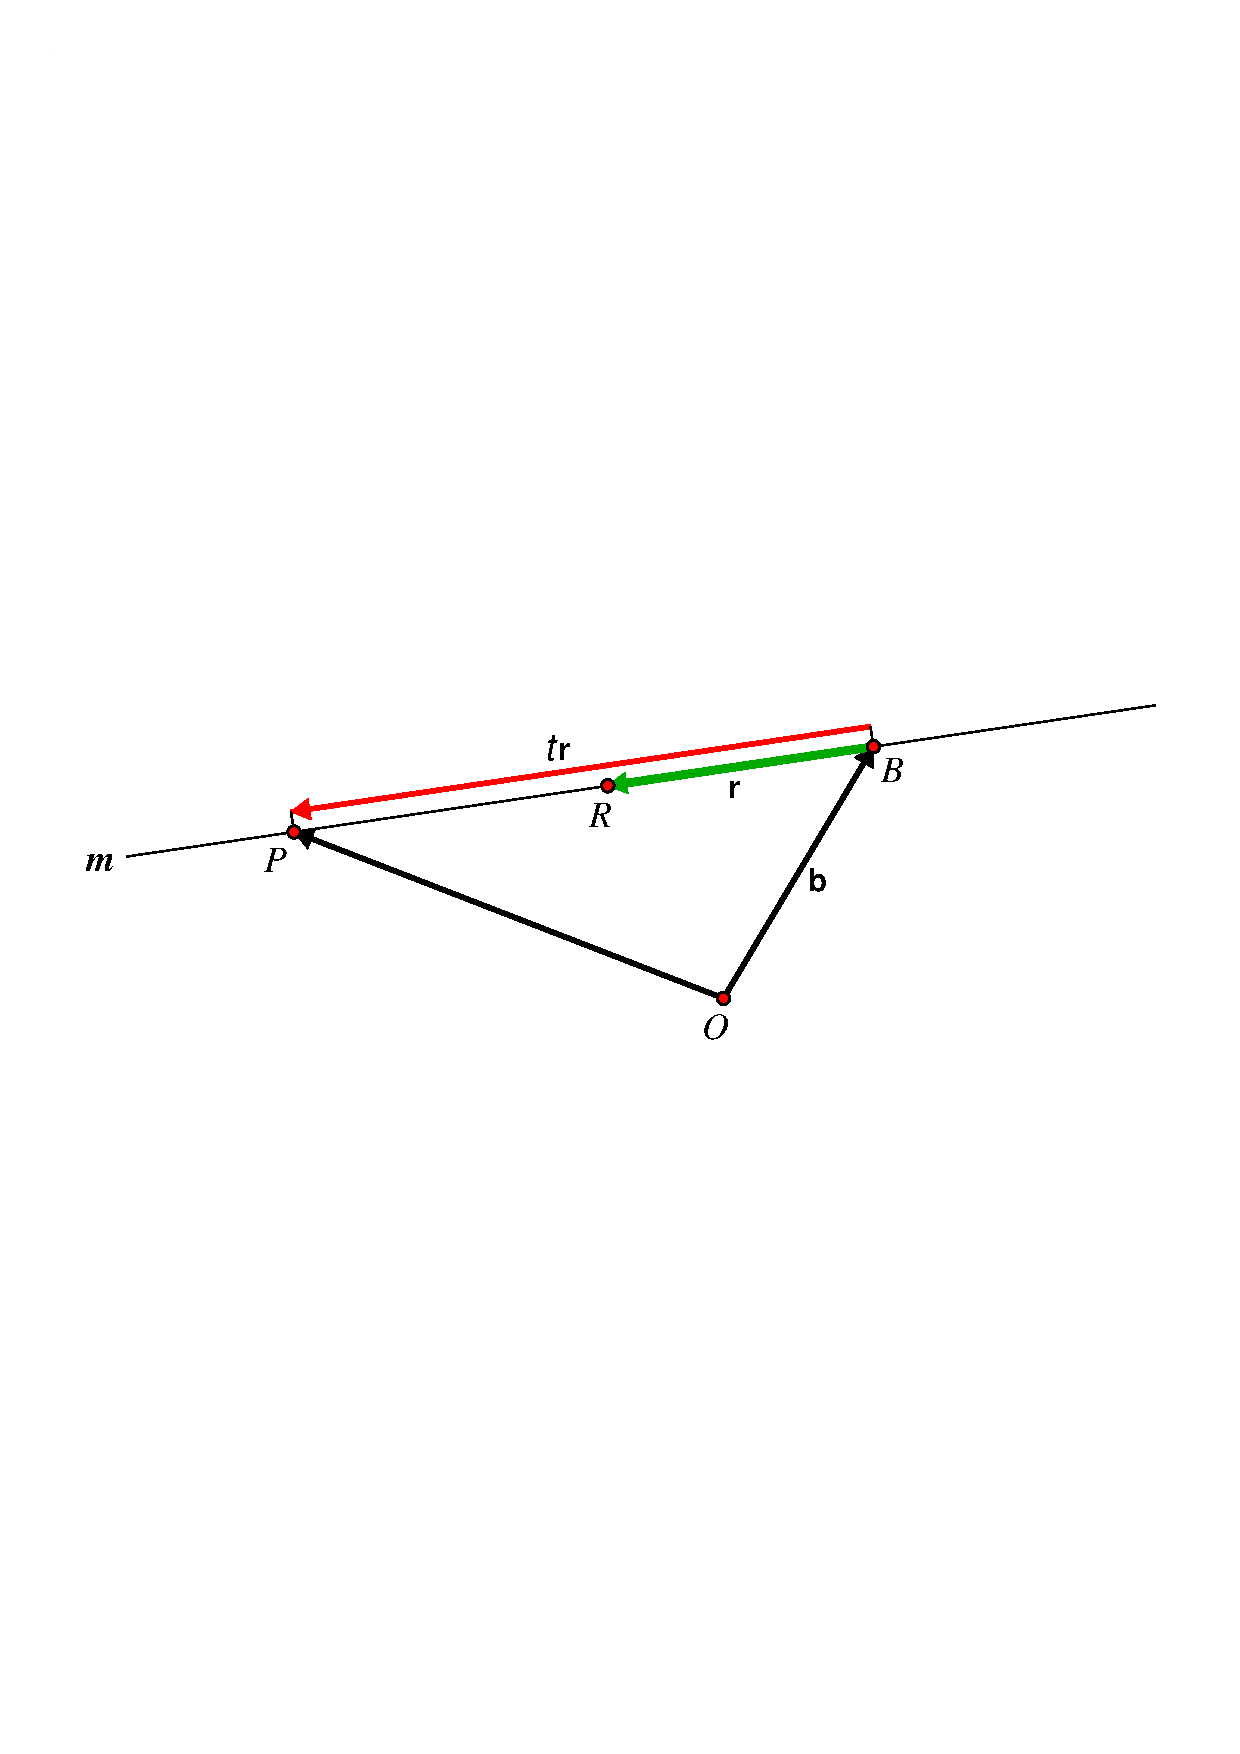
\includegraphics[trim=1cm 11.5cm 1cm
 11.5cm,width=0.60\textwidth,clip]{geometer/vektor8.pdf}
 \\Figur 6.5: Parameterfremstilling for linje 
\end{center}
Først vælges et \textit{begyndelsespunkt} $B$ på $m$, og vi sætter $\mathbf b=\stackrel{\rightarrow}{OB}$. Dernæst vælges et punkt $R \in m\,$ som ikke er det samme som $B$.  Vektoren $\mathbf r=\stackrel{\rightarrow}{BR}$ er da en retningsvektor for $\,m\,$. Til ethvert punkt $P$ på $\,m\,$ svarer der netop ét reelt tal $t$ der opfylder at $\stackrel{\rightarrow}{OP}=\mathbf b+t\mathbf r$. Omvendt svarer der til ethvert tal $t$ netop et punkt $P$ på $l$ så $\stackrel{\rightarrow}{OP}=\mathbf b+t\mathbf r$. Når $t$ \textit{gennemløber} de reelle tal fra -$\infty$ til +$\infty$, vil $P$ \textit{gennemløbe} hele $\,m\,$ i den retning som er bestemt ved $\mathbf r$. Man siger at 
$$\{\,P\,|\,\stackrel{\rightarrow}{OP}=\mathbf b +t\mathbf r\,\,\mathrm{hvor}\,\,t \in \mathbb R\,\}$$
er en parameterfremstilling for $\,m\,$.
\end{example}
Parameterfremstillinger kan også bruges til at beskrive linjestykker, det er emnet for den følgende opgave.
\begin{exercise}
Betragt situationen i eksempel \ref{tn6.linje}. Indtegn det orienterede linjestykke som har parameterfremstillingen
$$\{\,P\,|\,\stackrel{\rightarrow}{OP}=\mathbf b+t\mathbf r,\,\,\mathrm{hvor}\,\,t \in \left[\,- 1;\,2\,\right]\,\}\,.$$
\end{exercise}

Vi får brug for mere avancerede regneregler for addition af geometriske vektorer og multiplikation af geometriske vektorer med skalarer end dem vi har givet eksempler for ovenfor. De ridses op i den følgende sætning, og vi diskuterer bagefter eksempler på hvordan de kan begrundes ud fra de allerede definerede regneoperationer og sætninger kendt fra elementær geometri.\bs

\begin{theorem}[Regneregler] \label{tn6.regneregler}
For vilkårlige geometriske vektorer $ \mathbf u $, $ \mathbf v $ og $ \mathbf w $ og for vilkårlige reelle tal $ k_1 $ og $ k_2 $ gælder følgende regneregler: \smallskip \\
\begin{tabular}{lcl}
1. & $ \mathbf u + \mathbf v = \mathbf v + \mathbf u $ & Addition er kommutativ \smallskip \\
2. & $ (\mathbf u + \mathbf v ) + \mathbf w = \mathbf u + (\mathbf v + \mathbf w) $ & Addition er associativ \smallskip \\
3. & $ \mathbf u + \mnul = \mathbf u $ & Nulvektoren er neutral ved addition \smallskip  \\
4. & $ \mathbf u + (-\mathbf u) = \mnul $ & Summen af en vektor og dens modsatte er $\mnul$ \smallskip \\
%$ k_1 \mathbf u = \mathbf u k_1 $ & Produkt med skalar er kommutativ \smallskip \\
5. & $ k_1(k_2\mathbf u) = (k_1k_2)\mathbf u $ & Produkt med skalarer er associativ \smallskip \\
6. & $ (k_1 + k_2)\mathbf u = k_1\mathbf u + k_2\mathbf u $ & \multirow{2}{10cm}{$\biggr\rbrace$ De distributive regler gælder} \smallskip \\
7. & $ k_1(\mathbf u+\mathbf v) = k_1\mathbf u+ k_1 \mathbf v $ &  \smallskip  \\
8. & $ 1\mathbf u = \mathbf u $ & Skalaren $ 1 $ er neutral i produkt med vektorer \\
\end{tabular}
\end{theorem}

Regnereglerne i sætning \ref{tn6.regneregler} kan illustreres/eftervises ved hjælp af geometriske konstruktioner. Lad os som eksempel tage den første regel, den kommutative lov. Her behøver vi blot igen at rette blikket mod figuren i definition \ref{addition}\,, hvor $\mathbf u+\mv$ er konstrueret. Hvis vi nu konstruerer $\mv+\mathbf u$, skal vi  parallelforskyde linjestykket $OQ$ med $v$ og betragte det fremkomne linjestykke $RP_2$. Der må gælde at parallelogrammet $OQPR$ er identisk med parallelogrammet $OQP_2R$ hvorfor $P_2=P$ og dermed $\mathbf u+\mv=\mv+\mathbf u$.\\

I de følgende to opgaver opfordres læseren til selv at redegøre for to af de andre regneregler.
 
\begin{exercise}
Gør ved hjælp af figur 6.6 rede for regnereglen $ k(\mathbf u+\mathbf v) = k\mathbf u+ k \mathbf v $.
\begin{center}
		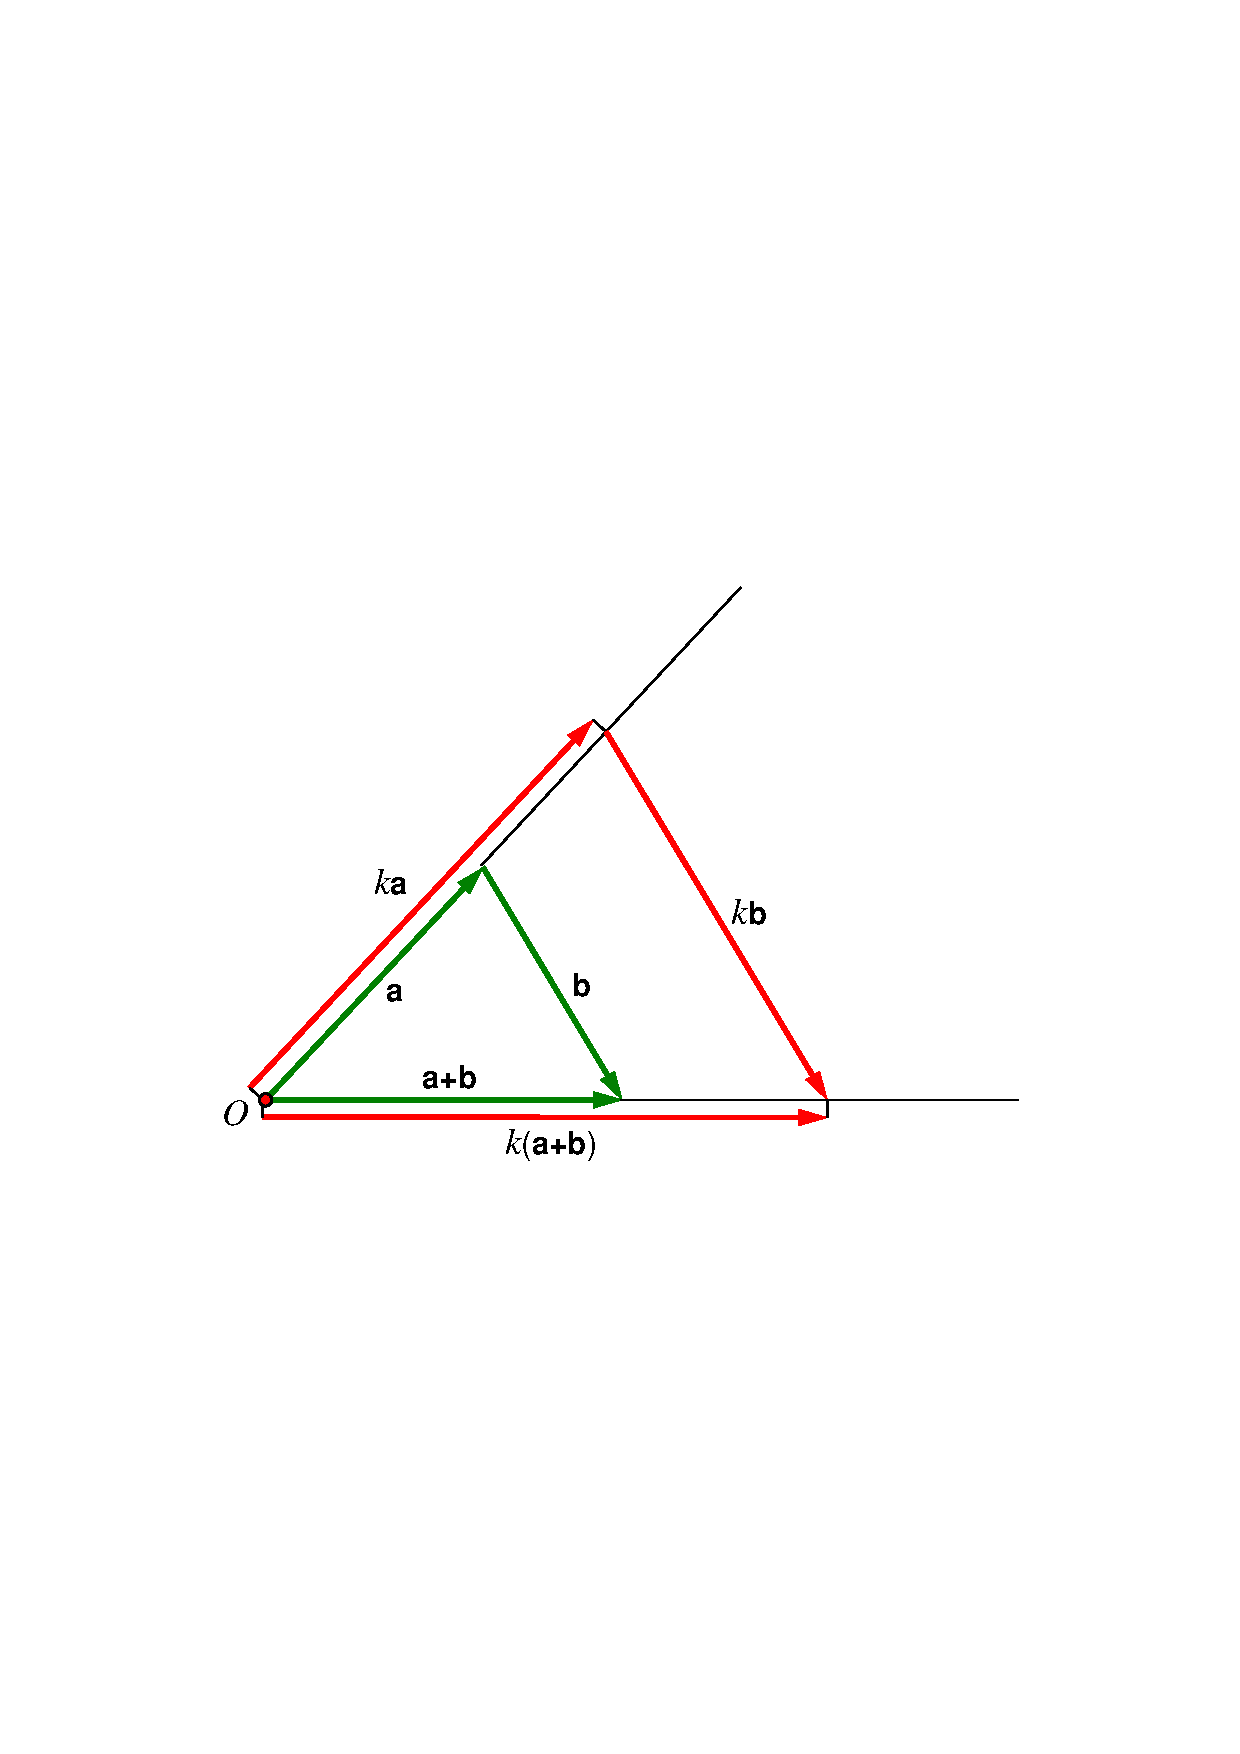
\includegraphics[trim=3.8cm 10cm 6cm 10.5cm,width=0.40\textwidth,clip]{geometer/vektor5.pdf}
		\\Figur 6.6			
\end{center}
\end{exercise}
\begin{exercise}
Tegn en figur som illustrerer regnereglen $ (\mathbf u + \mathbf v ) + \mathbf w = \mathbf u + (\mathbf v + \mathbf w) $.
\end{exercise}

For en given vektor $\mathbf u$ er det klart, at den modsatte vektor $-\mathbf u$ er den eneste vektor som opfylder ligningen $\mathbf u + \mathbf x=\mnul\,.$ For to vilkårlige vektorer $\mathbf u$ og $\mv$ er det også klart at der findes netop en vektor der opfylder ligningen
$\,\mathbf u + \mx=\mv\,,$ nemlig vektoren $\mx=\mv+(-\mathbf u)\,$ hvilket illustreres på figur 6.7.

\begin{center}
		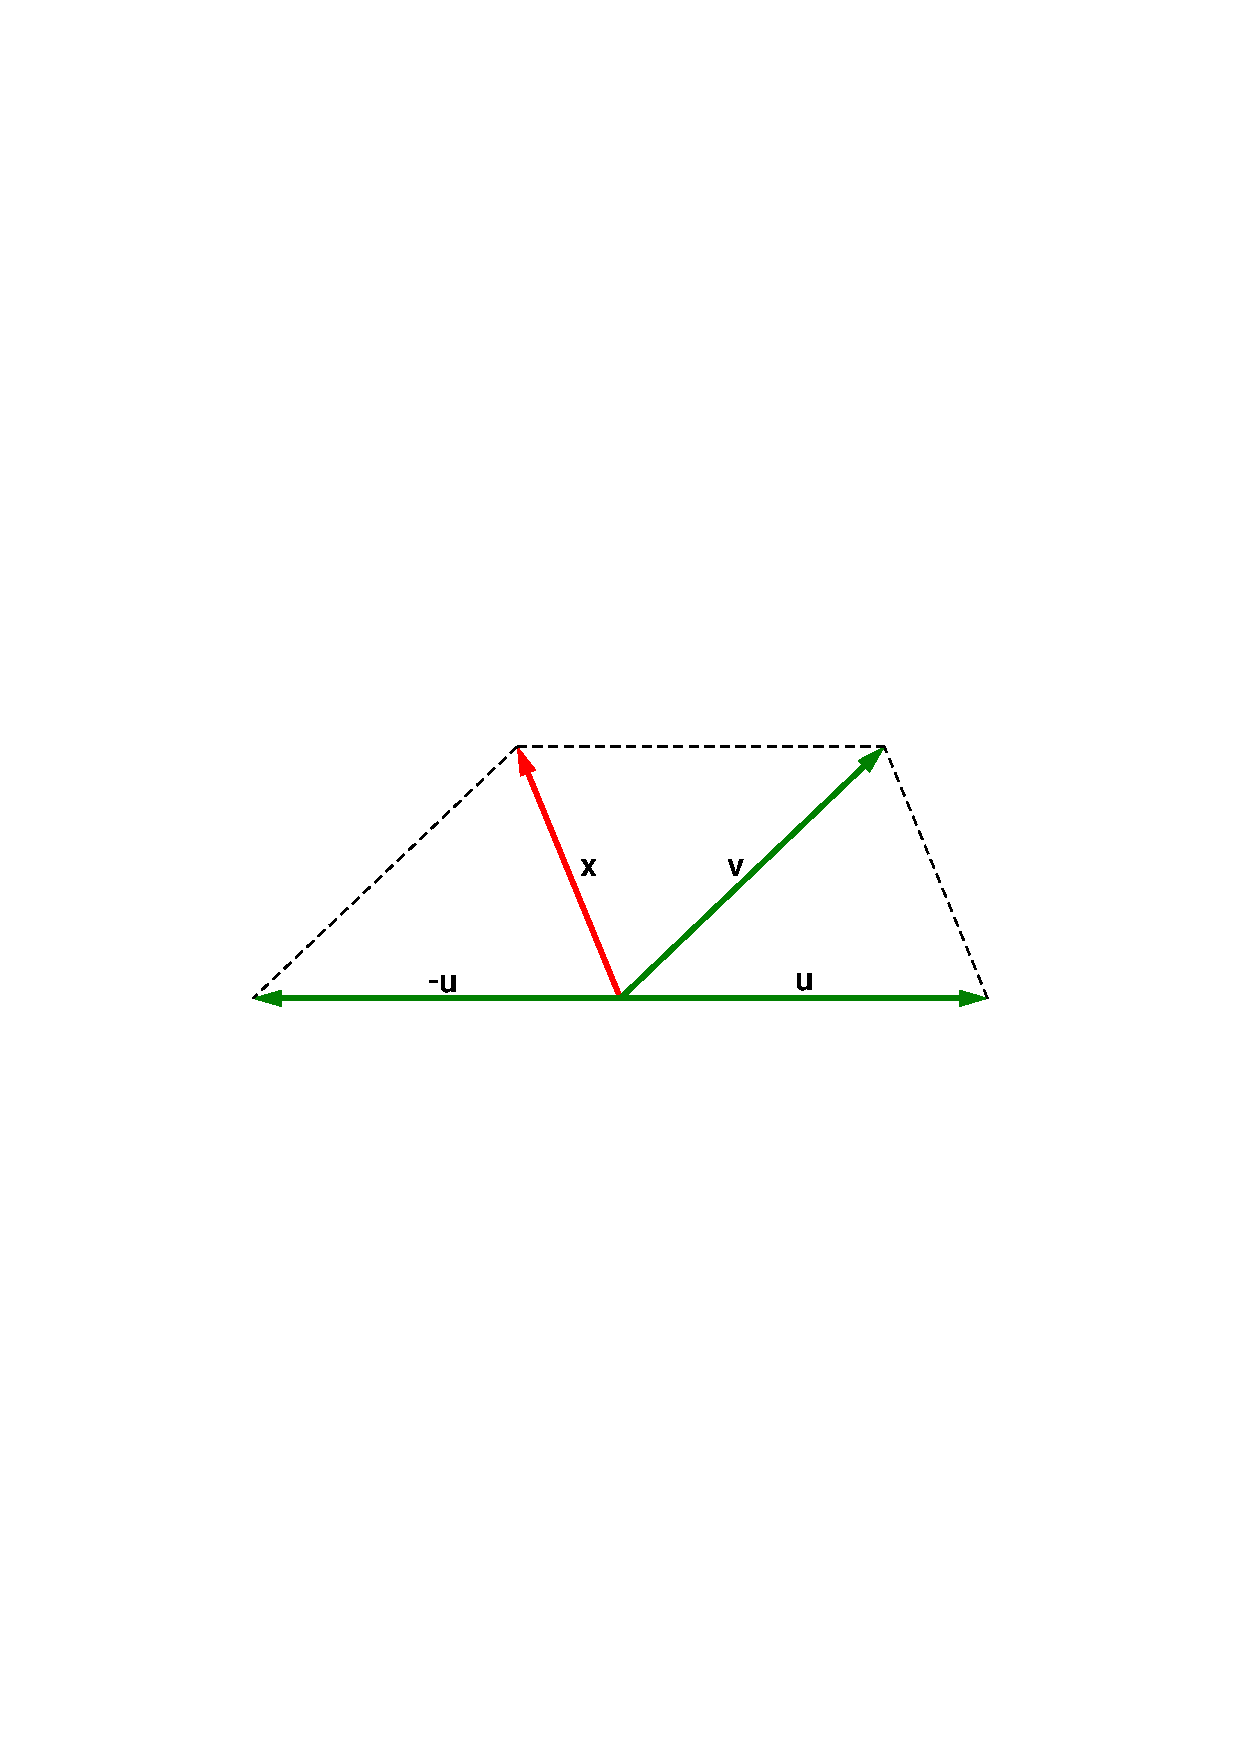
\includegraphics[trim=4cm 12.2cm 4cm 12.2cm,width=0.5\textwidth,clip]{geometer/vektor2subtr.pdf}
		\\Figur 6.7			
\end{center}

Vi kan derfor indføre \textit{subtraktion af vektorer} som en variant af addition således:\\

\begin{definition}[Subtraktion]
Ved differensen af to vektorer $\mathbf v$ og $\mathbf u$ forstås vektoren
\begin{equation}
\mv -\mathbf u = \mv+( -\mathbf u)\,.
\end{equation}
\end{definition}
 

\begin{aha}
Det er ikke nødvendigt at indføre højtidelig definition for \textit{division} af vektor med skalar, vi betragter den blot som en omskrivning af multiplikation med skalar:
%$$\mathrm{Subtraktion:}\quad\quad \mathbf u - \mathbf v =\mathbf u +(-\mathbf v)$$
$$\mathrm{Division\,\, med\,\, skalar:}\quad\quad\,\, \frac {\mathbf v} k = \frac 1 k \cdot \mathbf v$$
\end{aha}
%%%%%%%%%%%%%%%%%%%%%%%%%%%%%%%%%%%%%%%%%%%%%%%%%%%%%%%%%%
%%%%%%%%%%%%%%%%%%%%%%%%%%%%%%%%%%%%%%%%%%%%%%%%%%%%%%%%%%
%%%%%%%%%%%%%%%%%%%%%%%%%%%%%%%%%%%%%%%%%%%%%%%%%%%%%%%%%%
\section{Linearkombinationer}
En pointe ved regnereglen 
$\, (\mathbf u + \mathbf v ) + \mathbf w = \mathbf u + (\mathbf v + \mathbf w)\, $ fra sætning \ref{tn6.regneregler} er at man udelade parenteser når man skal addere en række vektorer, da det ingen betydning har for den resulterende vektor, i hvilken rækkefølge man har lagt vektorerne sammen. Dette er baggrunden \textit{linearkombinationer} hvor et sæt af vektorer er multipliceret med skalarer og derefter er opskrevet som en sum.\\

\begin{definition}[Linearkombination]
Når der er givet reelle tal $k_1,\,k_2,\ldots,k_n$ og i planen eller rummet vektorerne ${\mathbf v}_1,\,{\mathbf v}_2,\ldots,{\mathbf v}_n\,$ så kaldes summen
$$k_1{\mathbf v}_1+k_2{\mathbf v}_2+\ldots+k_n{\mathbf v}_n$$
en \ind{linearkombination}{linearkombination} af de $n$ givne vektorer.\\

Hvis alle koefficienterne $k_1,\cdots , k_n$ er lig med 0, kaldes linearkombinationen \textit{uegentlig}, men hvis blot én af dem er forskellig fra 0, er den \textit{egentlig}.
\end{definition}
\begin{example}[Konstruktion af en linearkombination]
\begin{center}
		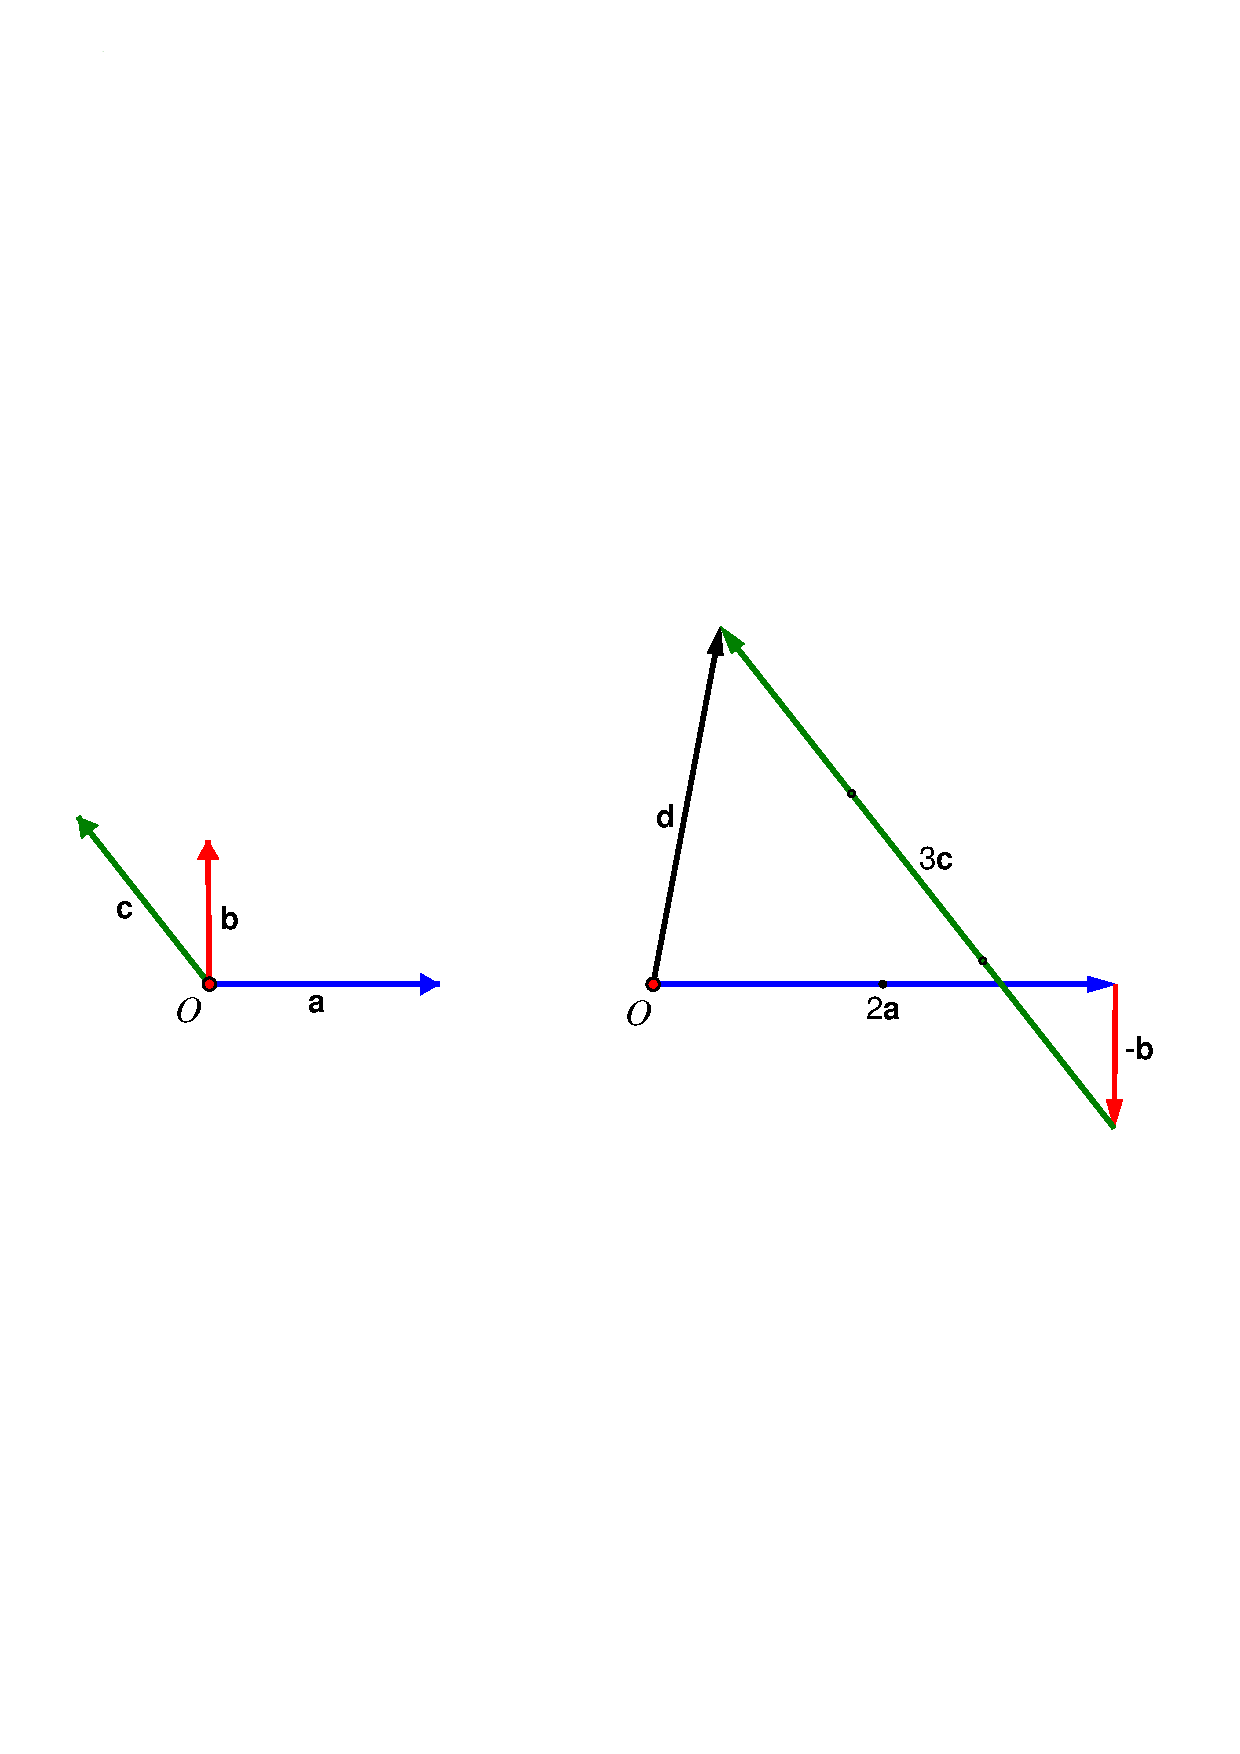
\includegraphics[trim=1.4cm 10.5cm 1.4cm 10.7cm,width=0.60\textwidth,clip]{geometer/vektor6.pdf}	
		\\Figur 6.9: Konstruktion af linearkombination			
\end{center}
På figur 6.9 til venstre er vektorerne $\mathbf a,\,\mathbf b\,\,\mathrm{og}\,\,\mathbf{c}$ indtegnet. På figuren til højre har vi konstrueret linearkombinationen 
$\mathbf d=2\mathbf a-\mathbf b +3\mathbf{c}$.
\end{example}


\begin{exercise}
Der er i planen givet vektorerne $\mathbf u,\,\mathbf v,\,\mathbf s\,\,\mathrm{og}\,\, \mathbf t$, samt parallelogrammet $A$, se figur 6.10.
\begin{center}
		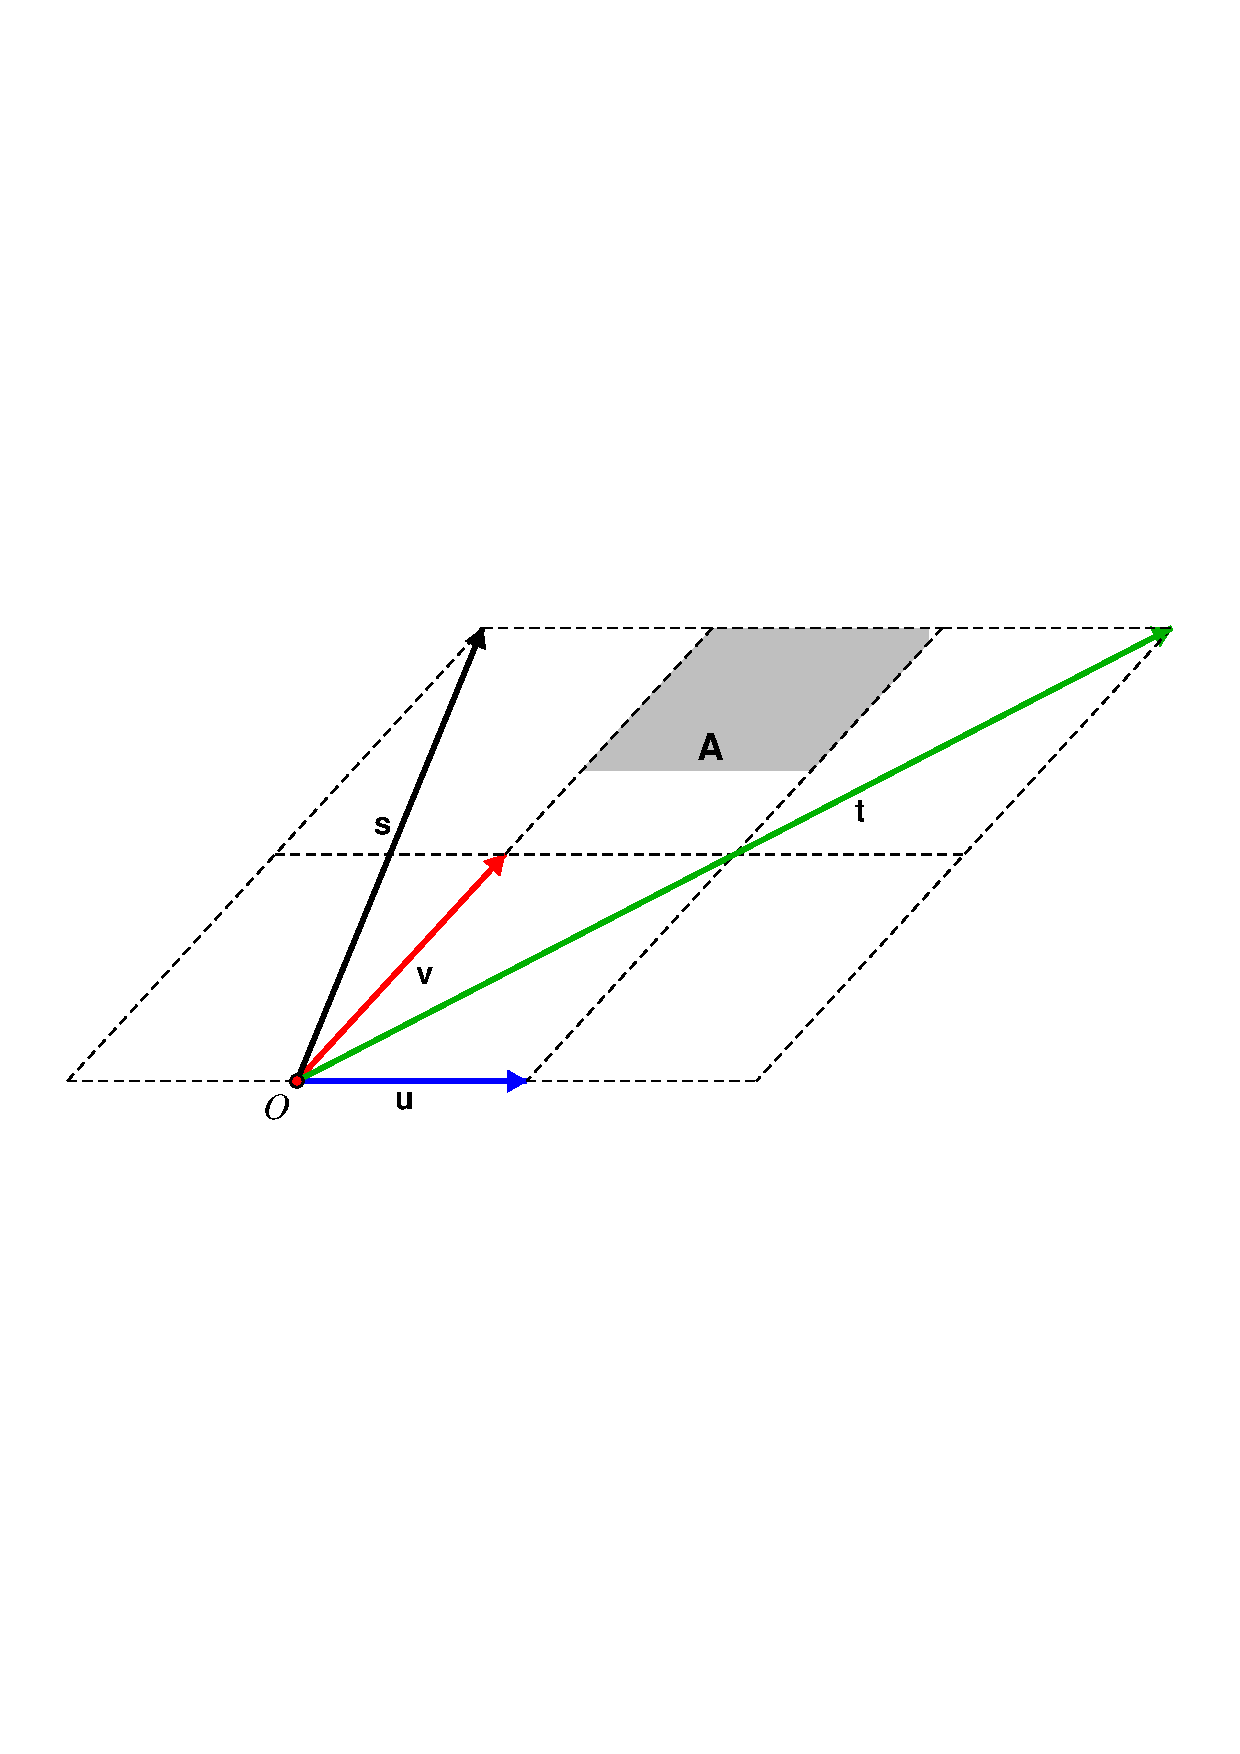
\includegraphics[trim=1cm 10.5cm 1cm 10cm,width=0.60\textwidth,clip]{geometer/vektor7.pdf}				
		\\Figur 6.10: Linearkombinationer
\end{center}
\begin{enumerate}
\item
Opskriv $\mathbf s$ som en linearkombination af $\mathbf u\,\, \mathrm{og}\,\,\mathbf v$.
\item
Vis at $\mathbf v$ kan udtrykkes ved linearkombinationen
$\,\,\mathbf v=\frac 13 \,\mathbf s+\frac 16 \,\mathbf t$.
\item
Indtegn linearkombinationen $\mathbf s+3\mathbf u -\mv .$
\item
Bestem reelle tal $a,\,b,\,c\,\,\mathrm{og}\,\,d$ således at $A$ kan beskrives ved \textit{parameterfremstillingen}
$$ A=
 \{\,P\,\big|\,
\stackrel{\rightarrow}{OP}=x\mathbf u+y\mathbf v\,\,\mathrm{hvor}\,\,x\in \left[\,a;\,b\,\right]\,\,\mathrm{og}\,\,y\in \left[\,c;\,d\,\right]
 \}\,.$$
\end{enumerate}
\end{exercise}

\section{Lineær afhængighed og lineær uafhængighed} \label{tn6.seclinafh}
Hvis to vektorer kan bringes til at ligge på den samme rette linje, siger man at de er \textit{lineært afhængige}. Det er klart at to egentlige vektorer er lineært afhængige hvis de er parallelle, i modsat fald er de \textit{lineært uafhængige}. Mere præcist kan vi sig om vekto\-rerne $\mathbf u$ og $\mathbf v$ at de er lineært afhængige hvis den ene af dem fremkommer af den anden ved multiplation med en skalar forskellig fra $0$, hvis der for eksempel findes et tal $k\neq 0$ således at
$$\mv=k\mathbf u\,.$$

Denne oprindelige betydning af begreberne lineær afhængighed og uafhængighed ønsker vi at generalisere sådan at begreberne kan bruges om et vilkårligt sæt  af vektorer. 

\begin{definition}[Lineær afhængighed og uafhængighed]\label{defLinAfh}
Et sæt af vektorer $(\mathbf v_1,\mathbf v_2,\ldots,\mathbf v_n)$ kaldes \ind{lineær afhængighed}{lineært afhængigt} hvis mindst én af vektorerne kan skrives som en linearkombination af de øvrige.\bs
%, for eksempel
%$$
%\mv_1=k_2\mv_2+k_3\mv_3+\cdots+k_{n}\mv_{n}.
%$$
Hvis ingen af vektorerne kan skrives som en linearkombination af de øvrige, kaldes sættet for \ind{lineær uafhængighed}{lineært uafhængigt}.\bs
NB: Et sæt som kun består af én vektor, kaldes for lineært afhængigt hvis vektoren er \textbf{0}-vektoren, og ellers lineært uafhængigt.
\end{definition}


\begin{example}[Lineært afhængige og lineært uafhængige vektorsæt]
I planen er givet tre vektorsæt $(\mathbf u,\mathbf v)$, $(\mathbf r,\mathbf s)$ og $(\mathbf a,\mathbf b,\mathbf c)\,,$ se figuren
\begin{center}
		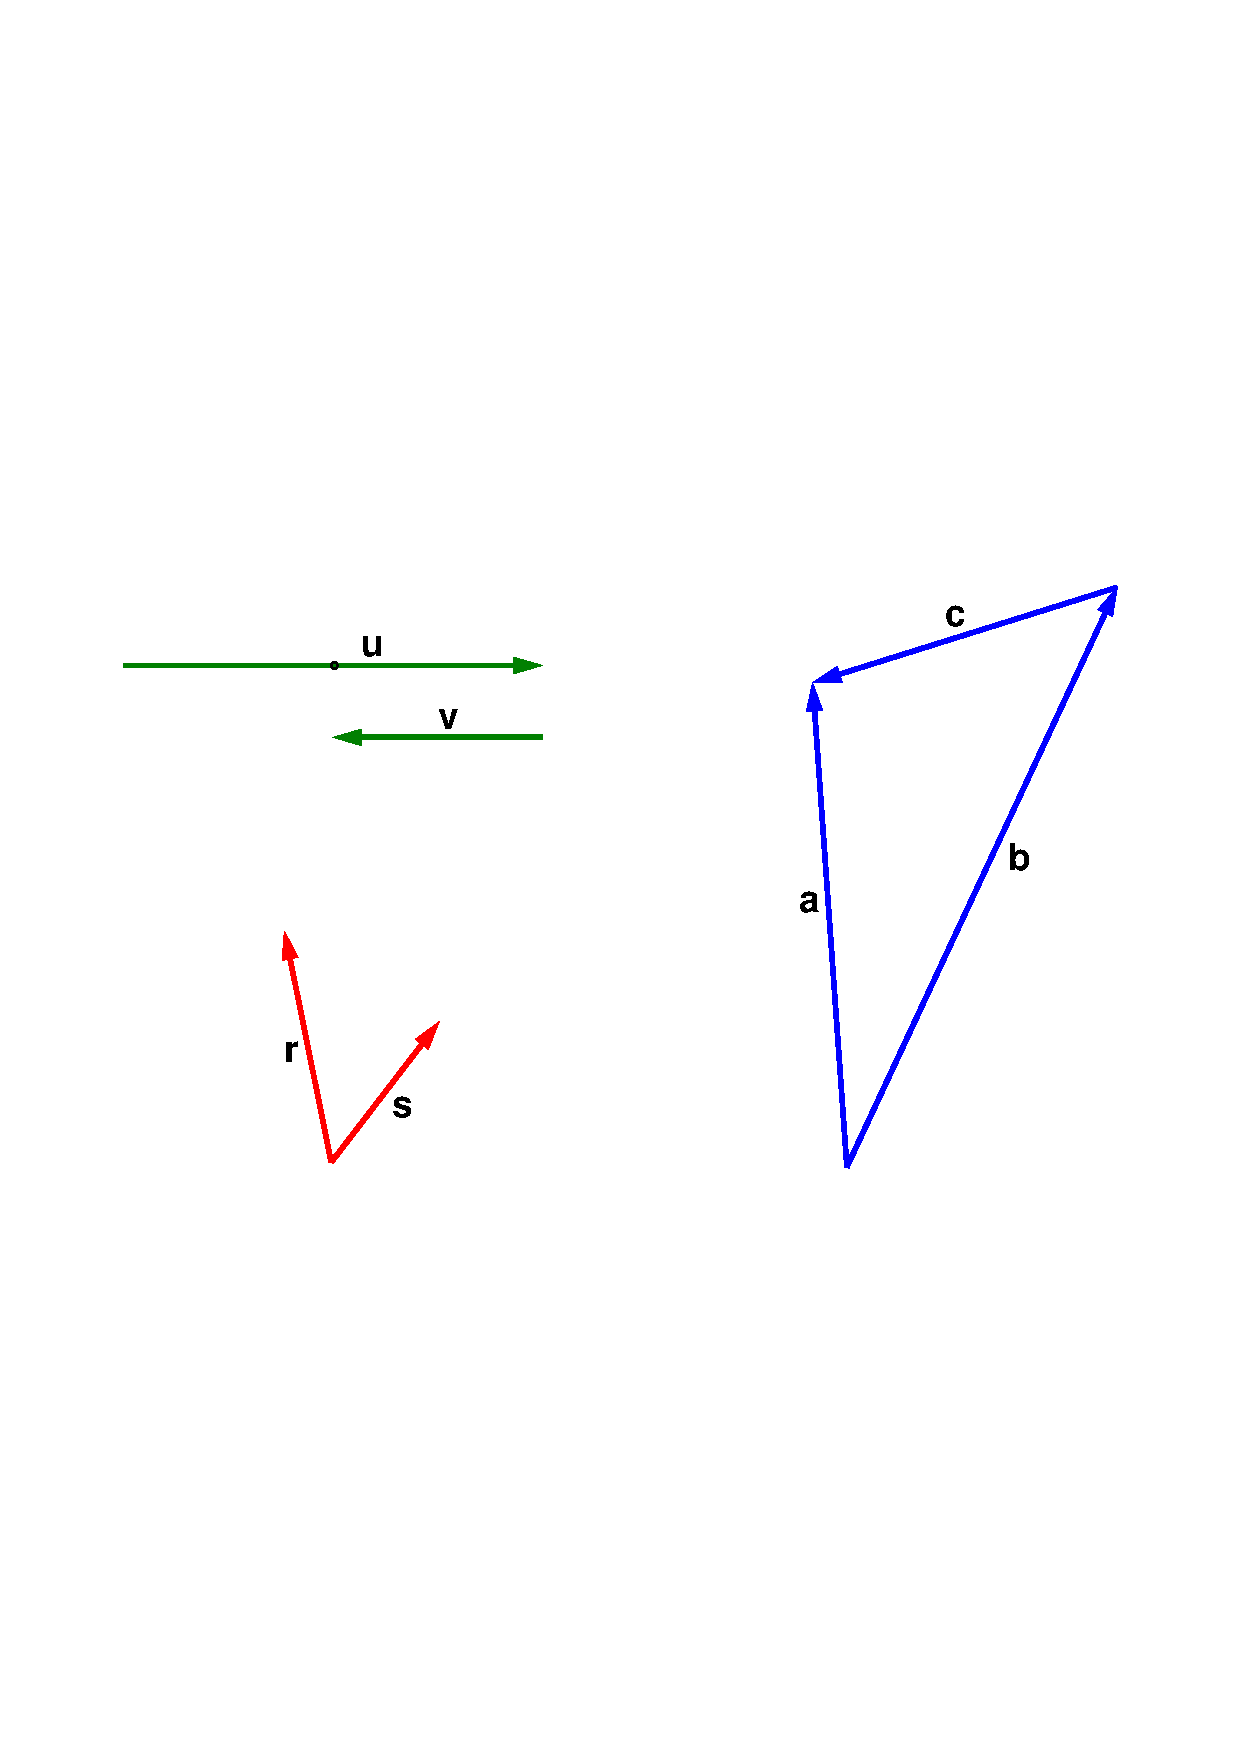
\includegraphics[trim=1.5cm 10cm 1.5cm 10cm,width=0.6\textwidth,clip]{geometer/vektor13.pdf}		
		\\Figur 6.11
\end{center}
Sættet $(\mathbf u,\mathbf v)$ er lineært afhængigt idet der for eksempel gælder $$\mathbf u =-2\mv\,.$$ Også sættet $(\mathbf a,\mathbf b,\mathbf c)$ er lineært afhængigt, da for eksempel $$\mb=\mc-\ma\,.$$
Kun sættet $(\mathbf r,\mathbf s)$ er lineært uafhængigt.
\end{example}

\begin{exercise}
Gør rede for at tre vektorer i rummet er lineært afhængige, hvis og hvis de kan bringes til at ligge i den samme plan. Hvilke betingelser må tre vektorer i rummet opfylde for at de er lineært uafhængige?
\end{exercise}
\begin{exercise}
Overvej det maksimale antal vektorer som et vektorsæt i planen kan rumme, hvis sættet skal være lineært uafhængigt. Samme spørgsmål for rummet. 
\end{exercise}

Når man skal undersøge om et sæt af vektorer er lineært uafhængigt eller lineært afhængigt, giver definition \ref{defLinAfh} ikke umiddelbart en praktisk fremgangsmåde. Det kan være nemmere at bruge sætningen der følger nedenfor. Den bygger på at et vektorsæt er lineært afhængigt hvis og kun hvis $\mnul$-vektoren kan opskrives som en egentlig linearkombination af vektorerne. Antag som en opvarmning til sætningen at sættet $(\ma,\mb,\mc)$ er lineært afhængigt fordi
$$\mathbf c=2\mathbf a-3\mathbf b.$$
Så kan $\mnul$-vektoren fremstilles ved den egentlige linearkombination
$$2\mathbf a-3\mathbf b-\mathbf c=\mathbf 0\,.$$
Antag omvendt at $\mnul$-vektoren er en egentlig linearkombination af vektorerne $\mathbf u, \mv$ og $\mathbf w$ således:
$$2\mathbf u-2\mathbf v +3\mathbf w=\mathbf 0\,.$$
Så har vi (for eksempel) at
$$\mathbf w=-\frac 2 3\mathbf u + \frac 2 3\mathbf v$$
og dermed at vektorer er lineært afhængige. 

\begin{theorem}[Lineær uafhængighed]\label{linafh}
Lad $k_1, k_2,\ldots,k_n$ være reelle tal. At vektorsættet $(\mathbf v_1,\mathbf v_2,\ldots,\mathbf v_n)$ er lineært uafhængigt, er ensbetydende med at ligningen
\begin{equation}\label{linafh_lign}
k_1{\mathbf v}_1+k_2{\mathbf v}_2+\cdots+k_n{\mathbf v}_n= \mathbf 0
\end{equation}
kun er opfyldt når alle koefficenterne $k_1, k_2,\ldots, k_n$ er lig med $0\,$.
\end{theorem}

\begin{bevis}
Antag at sættet $(\mathbf v_1,\mathbf v_2,\ldots,\mathbf v_n)$ er lineært afhængigt, og lad $v_i$ være en vektor som kan skrives som en linearkombination af de øvrige. Vi nyordner (om nødvendigt) sættet så $i=1$, hvorefter $\mv_1$ kan skrives på formen 
\begin{equation}
\mv1=k_2\mv_2+\cdots+k_n\mv_n
\,\,\Leftrightarrow\,\,
\mv1-k_2\mv_2-\cdots-k_n\mv_n=\mnul\,.
\end{equation}
$\mnul$-vektoren er hermed opskrevet på formen (\ref{linafh_lign}), hvor ikke alle koefficienter er $0\,$, idet koefficienten til $\mv_1$ er $1\,$.\bs
Antag omvendt at sættet er skrevet på formen (\ref{linafh_lign}), og lad $k_i\neq 0\,.$ Vi nyordner (om nødvendigt) sættet så $i=1$ hvorefter vi har
\begin{equation}
k_1\mv1=-k_2\mv_2-\cdots-k_n\mv_n
\,\,\Leftrightarrow\,\,
\mv1=-\frac{k_2}{k_1}\mv_2-\cdots-\frac{k_n}{k_1}\mv_n\,.
\end{equation}
Heraf ses det at sættet er lineært afhængigt.
\end{bevis}

\begin{example}[Lineært afhængigt sæt]
Ethvert vektorsæt som indeholder nul-vektoren, er det lineært afhængigt. Betragt for eksempel sættet $(\mathbf u,\mv,\mnul,\mathbf w)$. Det er oplagt at nul-vektoren kan skrives som linearkombination af de øvrige tre vektorer:
$$
\mnul=0\mathbf u+0\mv+0\mathbf w\,,
$$hvor nul-vektoren er skrevet som en linearkombination af de øvrige vektorer i sættet.
\end{example}

\textit{Parameterfremstillinger for planer} i rummet opstilles ved hjælp af to lineært uafhængige vektorer. Nedenfor giver vi først et eksempel på en plan der indeholder origo, dernæst et eksempel på en plan der ikke indeholder origo.
\begin{example}[Parameterfremstilling for en plan]\label{tn6.planRum1}
Der er givet en plan i rummet som går gennem origo, se figur 6.12. Vi ønsker at beskrive punkterne i planen ved hjælp af en \ind{parameterfremstilling}{parameterfremstilling}.
\begin{center}
		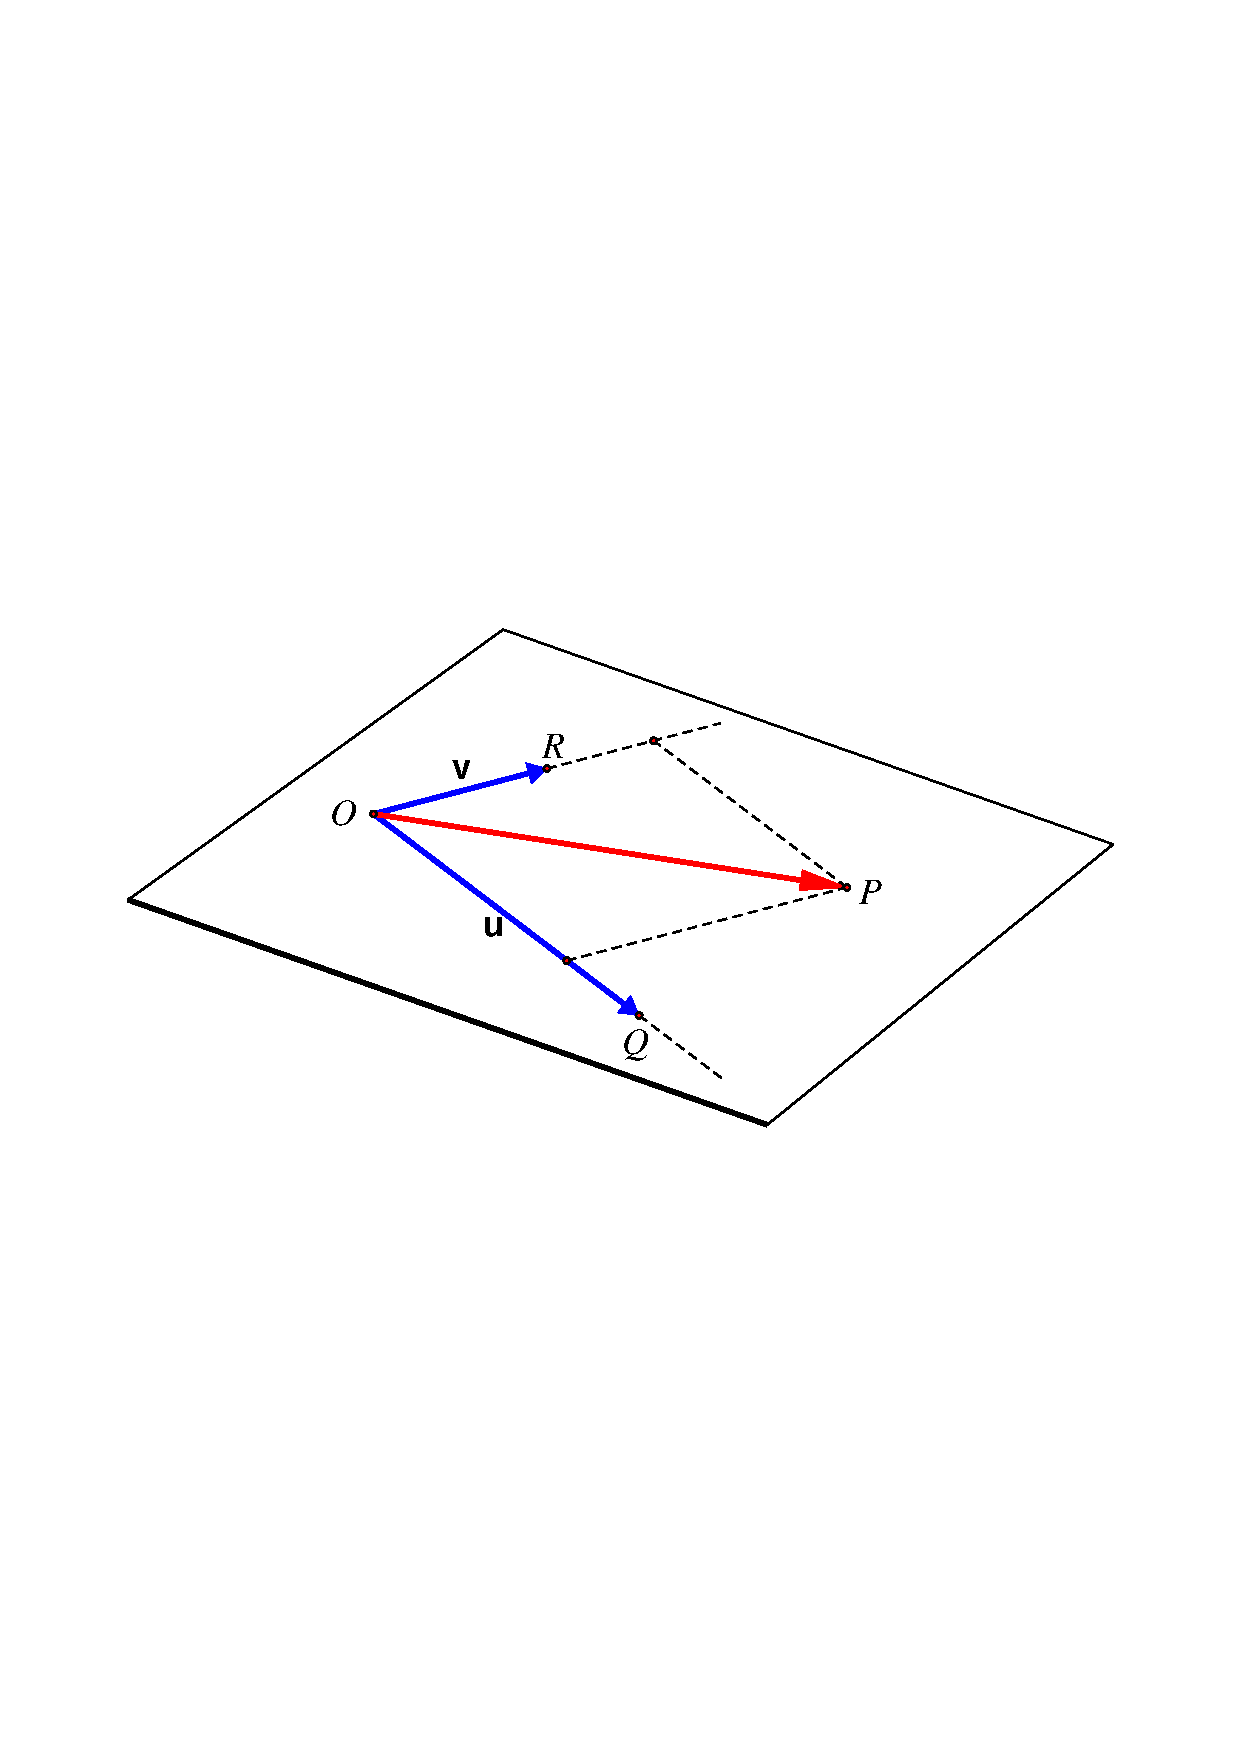
\includegraphics[trim=2cm 10cm 2cm
 10cm,width=0.60\textwidth,clip]{geometer/vektor14.pdf}
  \\Figur 6.12: En plan i rummet gennem origo		
 
\end{center}
På den givne plan vælges to punkter $Q$ og $R$ som ikke er origo, og som ikke ligger på en fælles linje gennem origo. Vektorerne $\mathbf u=\stackrel{\rightarrow}{OQ}$ og $\mathbf v=\stackrel{\rightarrow}{OR}$ vil da være lineært uafhængige, og kaldes for planens \ind{retningsvektor}{retningsvektorer}. Til ethvert punkt $P$ i planen findes der netop ét reelt talpar $(s,t)$ således at  
$\stackrel{\rightarrow}{OP}=s\mathbf u+t\mathbf v\,$. Omvendt findes der til ethvert reelt talpar $(s,t)$ netop et punkt $P$ i planen som opfylder $\stackrel{\rightarrow}{OP}=s\mathbf u+t\mathbf v\,$. Man siger at
$$
\{P\,|\, \stackrel{\rightarrow}{OP}=s\mathbf u+t\mathbf v\,;\,\,(s,t)\in \mathbb R^2\}
$$
er en parameterfremstilling af den givne plan.
\end{example}
\begin{example}[Parameterfremstilling for en plan]\label{tn6.planRum2}
En plan i rummet går ikke gennem origo, vi ønsker at beskrive den ved hjælp af en para\-meterfremstilling.
\begin{center}
		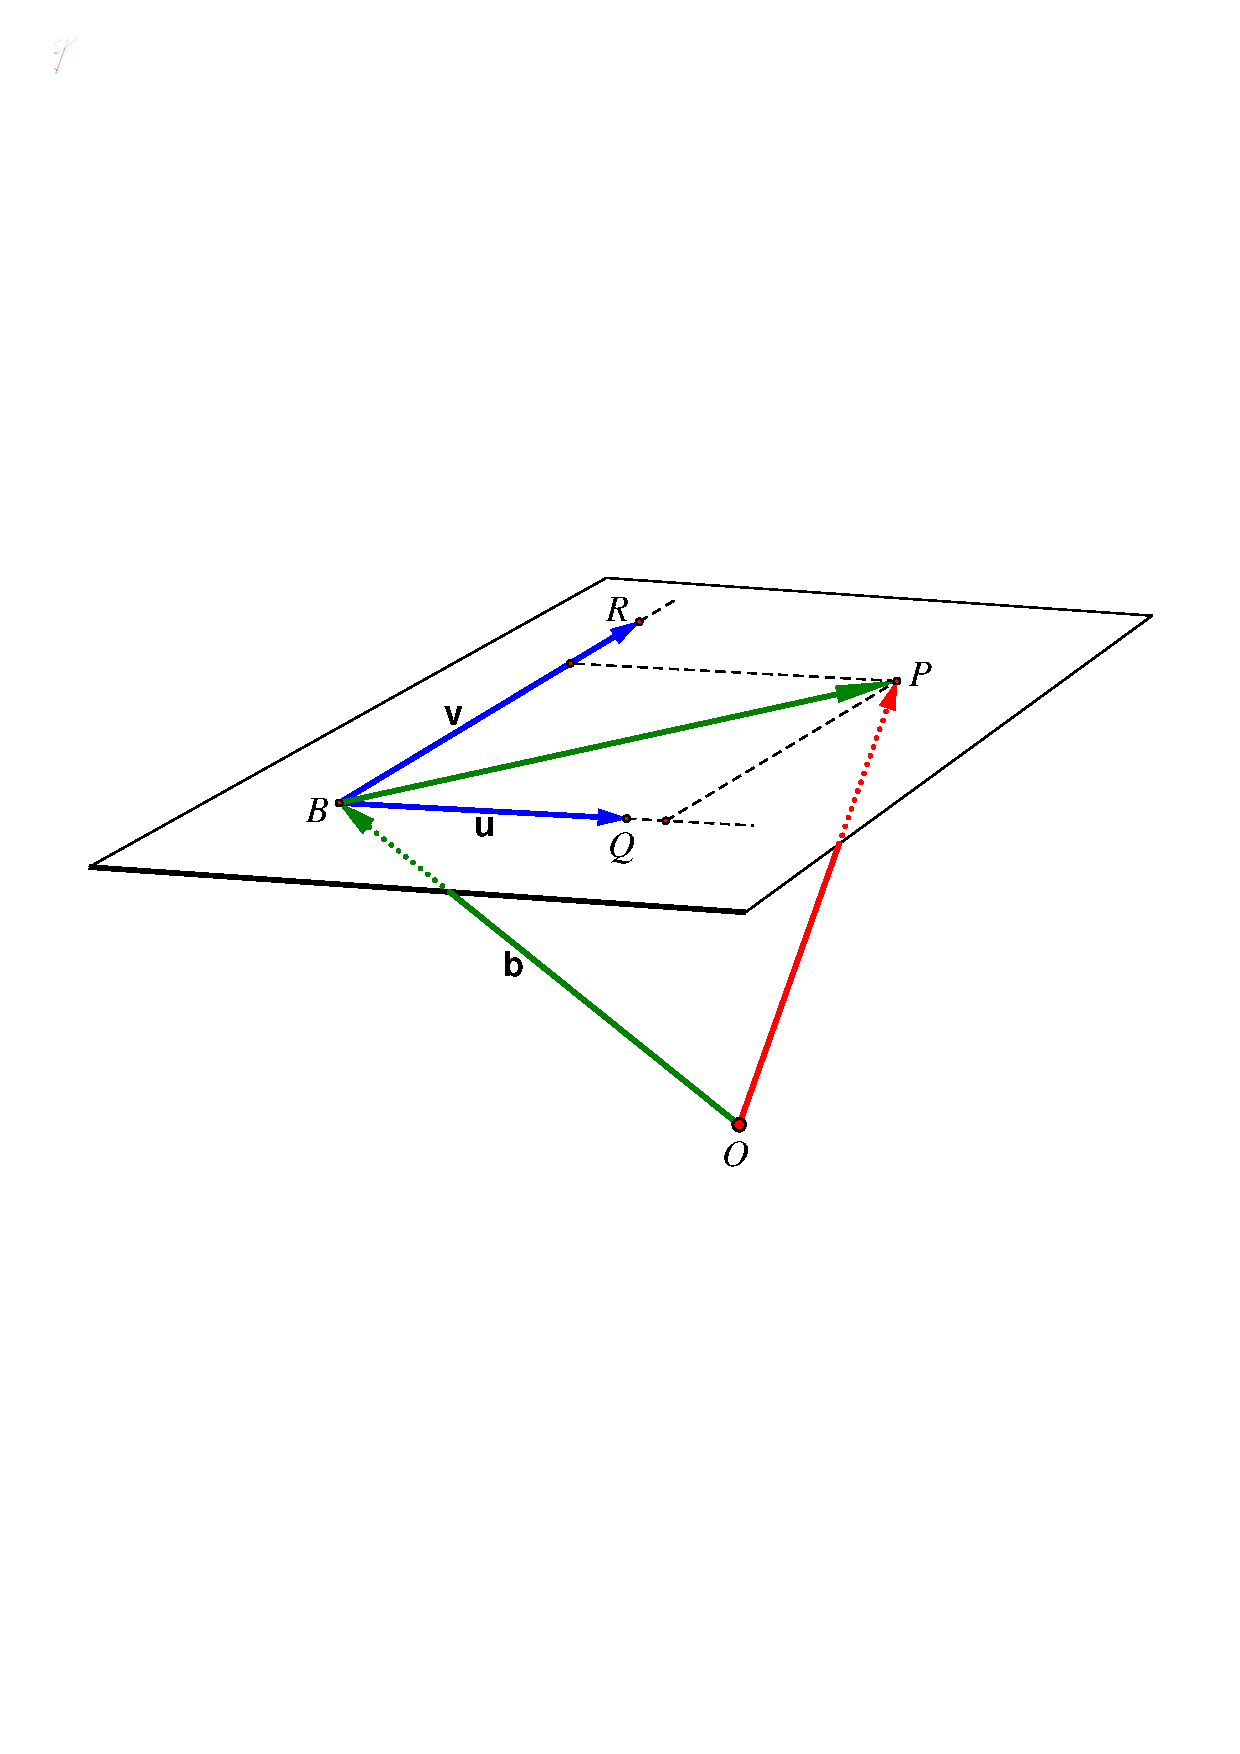
\includegraphics[trim=1.5cm 9cm 1.5cm
 9cm,width=0.65\textwidth,clip]{geometer/vektor15.pdf}	
   \\Figur 6.13: En plan i rummet	
\end{center}
Først vælges der et begyndelsespunkt $B$ på planen, og vi sætter $\mathbf b=\stackrel{\rightarrow}{OB}$. Dernæst vælges der to lineært uafhængige retningsvektorer $\mathbf u=\stackrel{\rightarrow}{BQ}$ og $\mathbf v=\stackrel{\rightarrow}{BR}$ hvor $Q$ og $R$ ligger på planen. Til ethvert punkt $P$ på planen findes der så netop ét reelt talpar $(s,t)$, således at  
$$\stackrel{\rightarrow}{OP}=\stackrel{\rightarrow}{OB}+\stackrel{\rightarrow}{BP}=\mathbf b+s\mathbf u+t\mathbf v\,.$$
Omvendt findes der til ethvert reelt talpar $(s,t)$ netop et punkt $P$ i planen som denne vektorligning. Man siger at
$$
\{P\,|\, \stackrel{\rightarrow}{OP}=\mathbf b+s\mathbf u+t\mathbf v\,;\,\,(s,t)\in \mathbb R^2\}
$$
er en parameterfremstilling for den givne plan.
\end{example}
\begin{exercise}
Giv en parameterfremstilling for det i planen liggende parallelogram $A$:
\begin{center}
		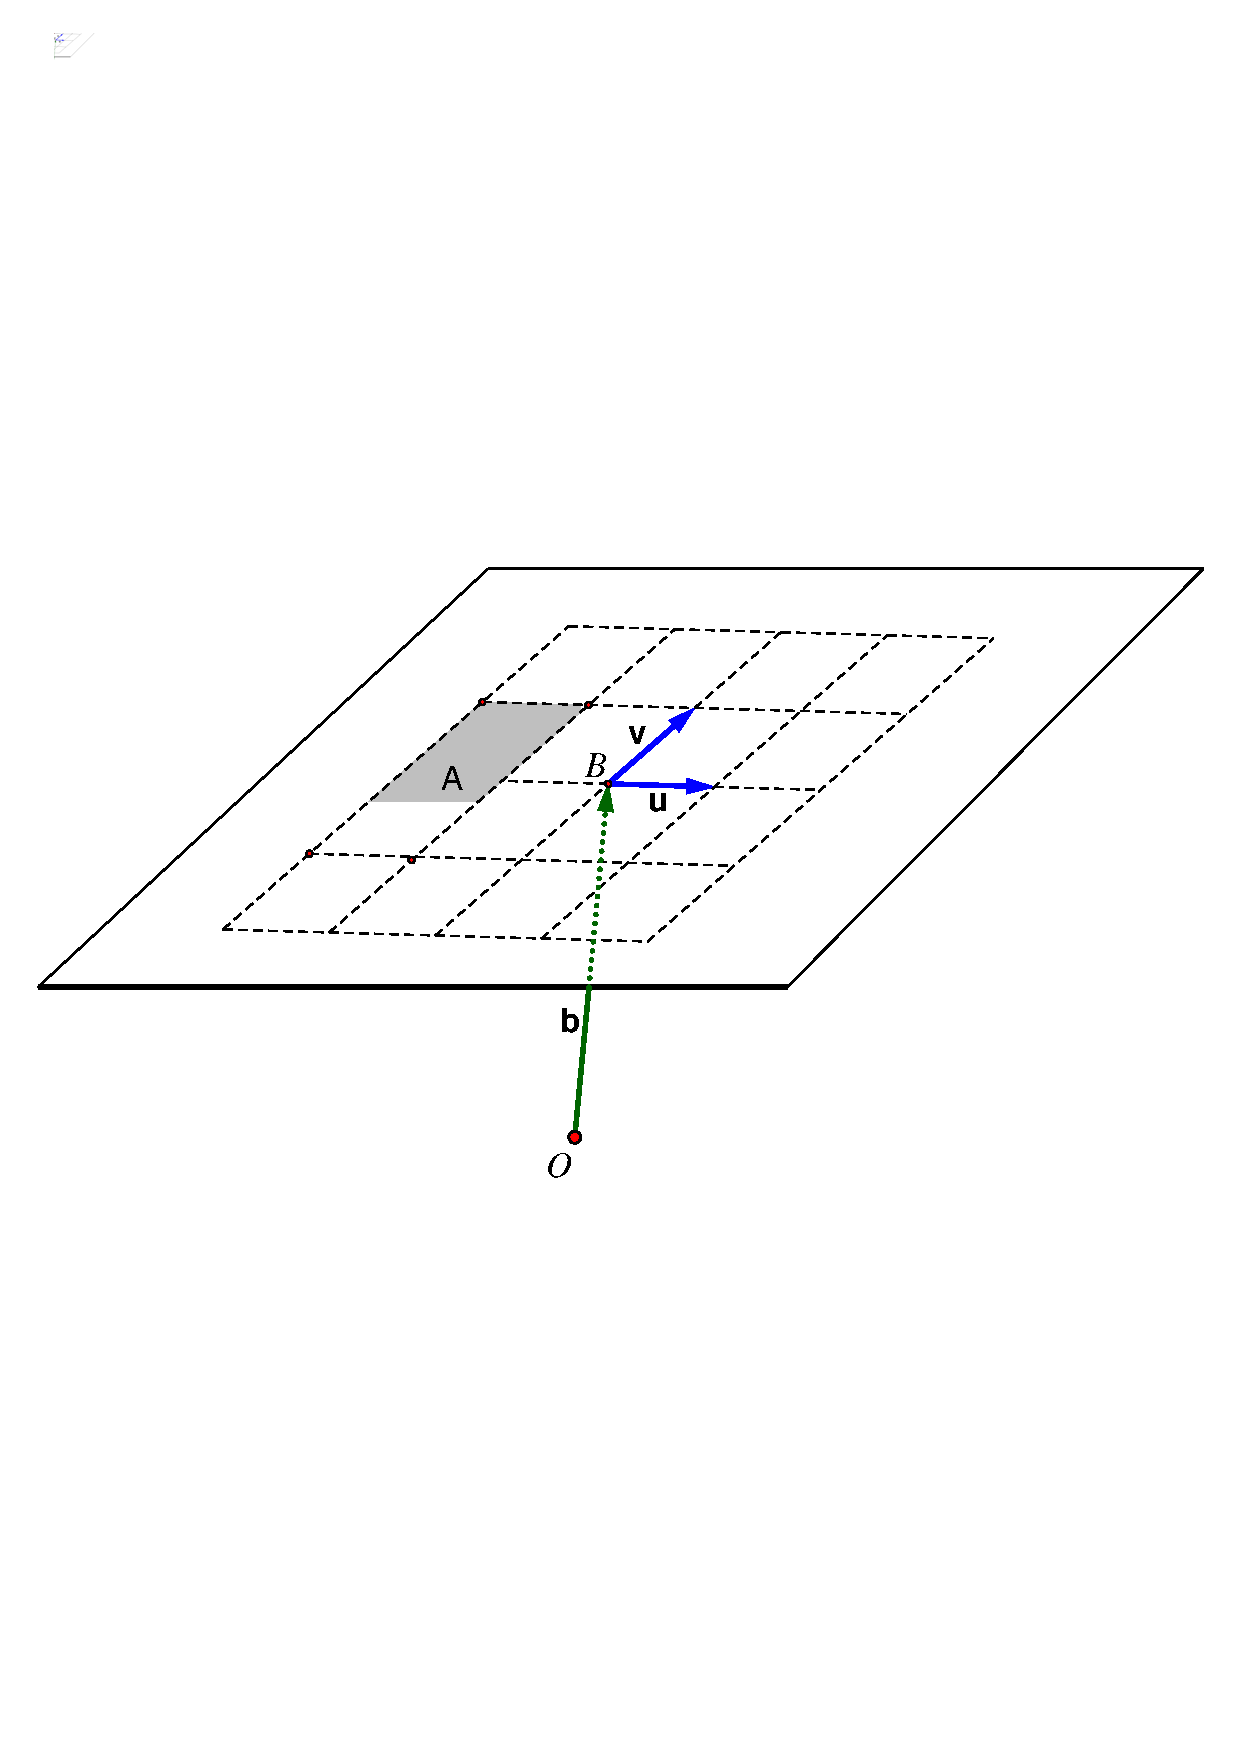
\includegraphics[trim=0.7cm 9cm 0.7cm
 9cm,width=0.60\textwidth,clip]{geometer/vektor16.pdf}		
   \\Figur 6.14
\end{center}
\end{exercise}
%%%%%%%%%%%%%%%%%%%%%%%%%%%%%%%%%%%%%%%%%%%%%%%%%%%%%%%%%%
%%%%%%%%%%%%%%%%%%%%%%%%%%%%%%%%%%%%%%%%%%%%%%%%%%%%%%%%%%
%%%%%%%%%%%%%%%%%%%%%%%%%%%%%%%%%%%%%%%%%%%%%%%%%%%%%%%%%%
\section{De sædvanlige baser i planen og rummet}
I den \textit{analytiske geometri} viser man hvordan tal og ligninger kan beskrive geometriske objekter og fænomener, herunder vektorer. Her er begrebet koordinater afgørende. Det handler om hvordan vi kan fastlægge de geometriske objekters placering i rummet og i forhold til hinanden ved hjælp af tal og talsæt. For at få grundlaget i orden skal vi vælge et vist antal vektorer, som vi udnævner til \ind{basisvektor}{basisvektorer}. Basisvektorerne \ind{ordnet sæt}{ordnes}, det vil sige forsynes med en bestemt rækkefølge, og de udgør derefter en \ind{basis}{basis}. Når en basis er givet, kan alle vektorer beskrives ved hjælp af koordinater, som vi samler i såkaldte koordinatvektorer. Hvordan hele denne procedure foregår, udfolder vi først gennem de sædvanlige ortonormale baser i planen og rummet. Senere kommer vi ind på at det ofte kan være hensigtsmæssigt at benytte andre baser end de sædvanlige, og hvordan relationen mellem en vektors koordinater er i forskellige baser.

\begin{definition}[Standardbasis i planen]
Ved en \ind{standardbasis}{standardbasis} eller en \ind{e-basis}{e-basis} for de geometriske vektorer i planen forstås et ordnet sæt af to vektorer $(\mathbf i,\mathbf j)$ som opfylder:
\begin{itemize}
\item
$\mathbf i$ og $\mathbf j$ har begge længden 1.
\item
$\mathbf i$ og $\mathbf j$ er ortogonale (vinkelrette).
\item
Stedvektoren for $\mathbf j$ fremkommer når stedvektoren for $\mathbf i$ drejes omkring origo med vinklen $\frac \pi 2$ mod uret.
\end{itemize}
Når $(\mathbf i,\mathbf j)$ er en e-basis, forstås ved et $(O,\mathbf i,\mathbf j)$-koordinatsystem et sædvanligt retvinklet $(X,Y)$-koordinatsystem hvor $X$-aksen har origo som startpunkt og $\mathbf i$ som retningsvektor, mens $Y$-aksen har origo som startpunkt og $\mathbf j$ som retningsvektor.
\begin{center}
		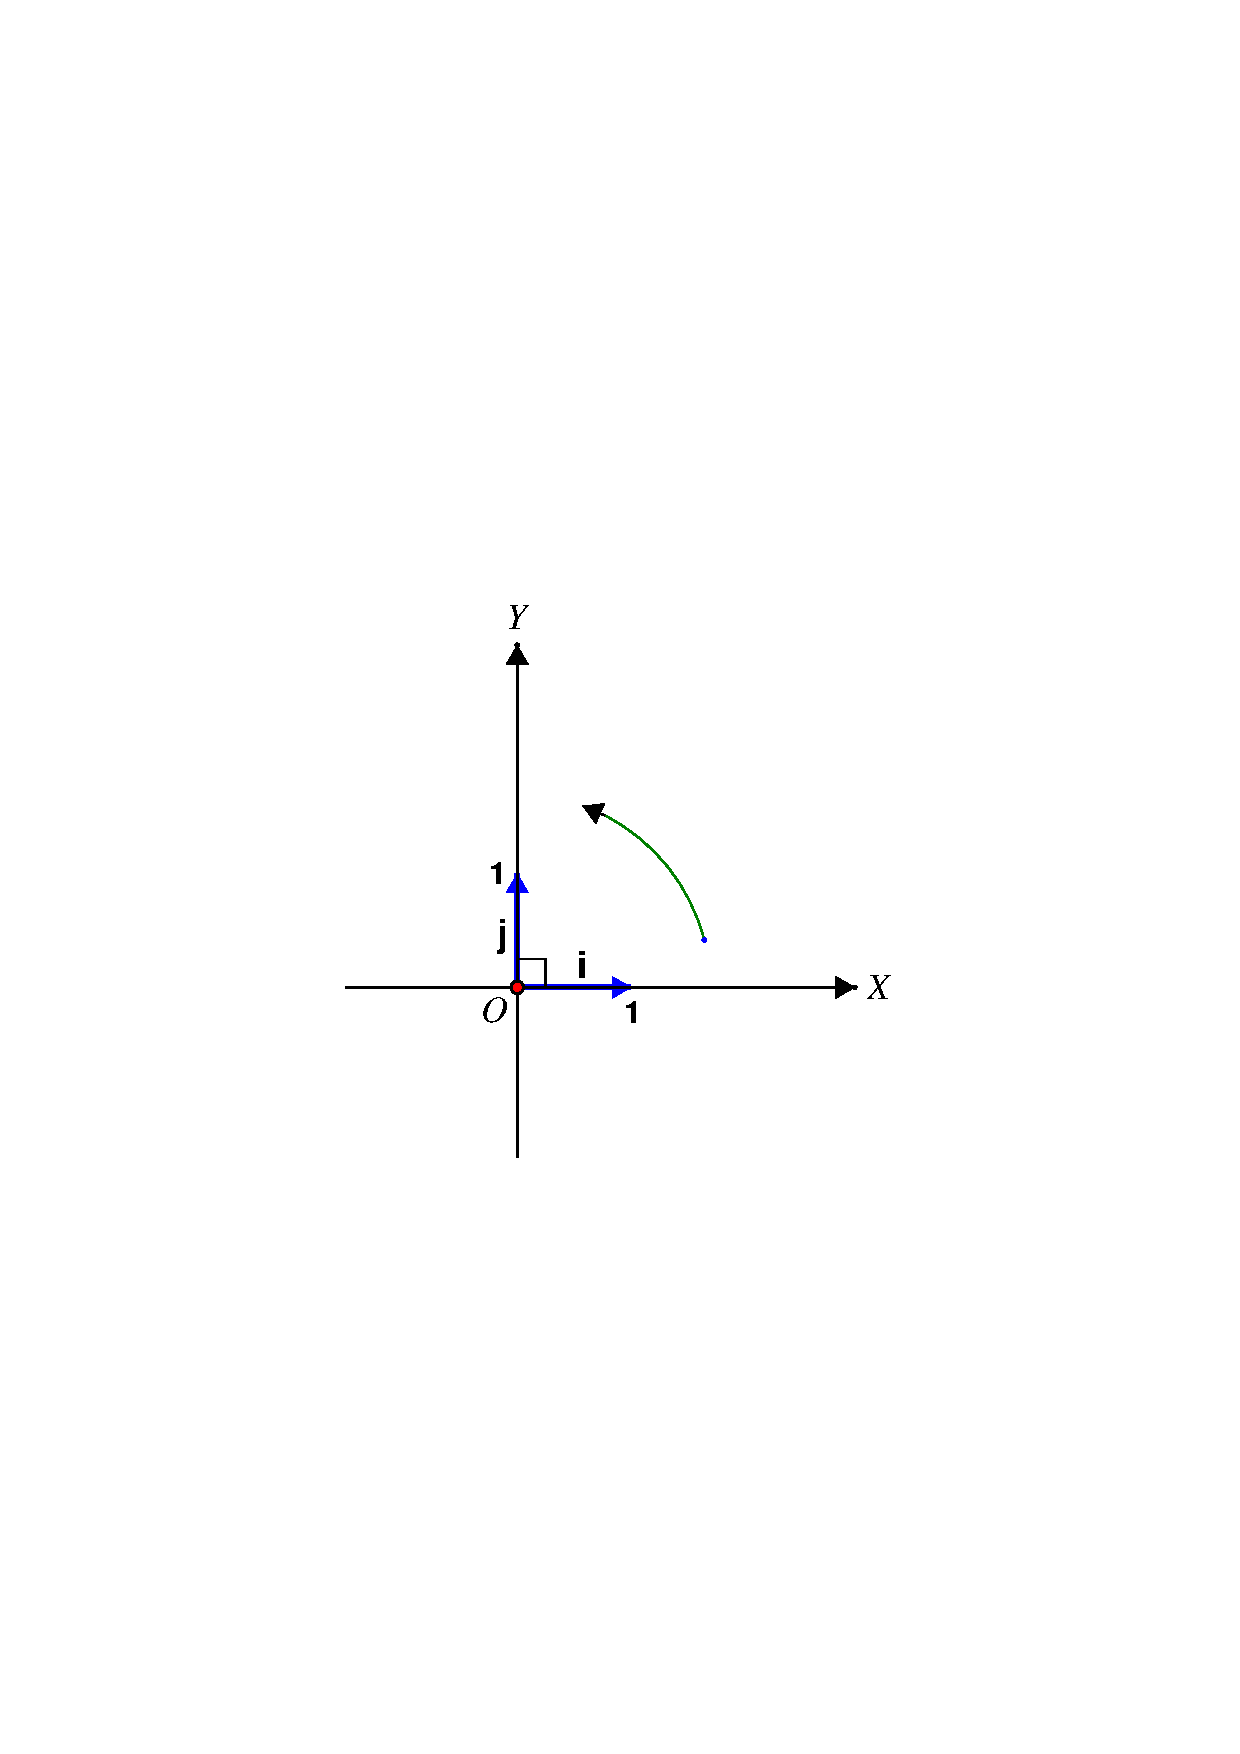
\includegraphics[trim=6.5cm 11cm 5cm 10cm,width=0.30\textwidth,clip]{geometer/vektor9.pdf}				
		\\Figur 6.15: Sædvanligt retvinklet koordinatsystem i planen
\end{center}
\end{definition}

\begin{theorem}[En vektors $e$-koordinater]
Når $(\mathbf i,\mathbf j)$ er en e-basis, kan enhver vektor $\mathbf v$ i planen på netop én måde skrives som en linearkombination af $\mathbf i$ og $\mathbf j$:
$$\mathbf v=x\mathbf i+y\mathbf j.$$
Koefficienterne $x$ og $y$ i linearkombinationen kaldes for $\mathbf v$'s \textit{koordinater med hensyn til e-basis}, eller kortere $\mathbf v$'s e-koordinater, og de samles i en \ind{koordinatvektor}{koordinatvektor} med følgende skrivemåde:
$$_\mathrm e\mathbf v=
\begin{matr}{r}x\\y\end{matr}\,.
$$

\end{theorem}

\begin{remark}[Et punkts koordinater]

\begin{center}
		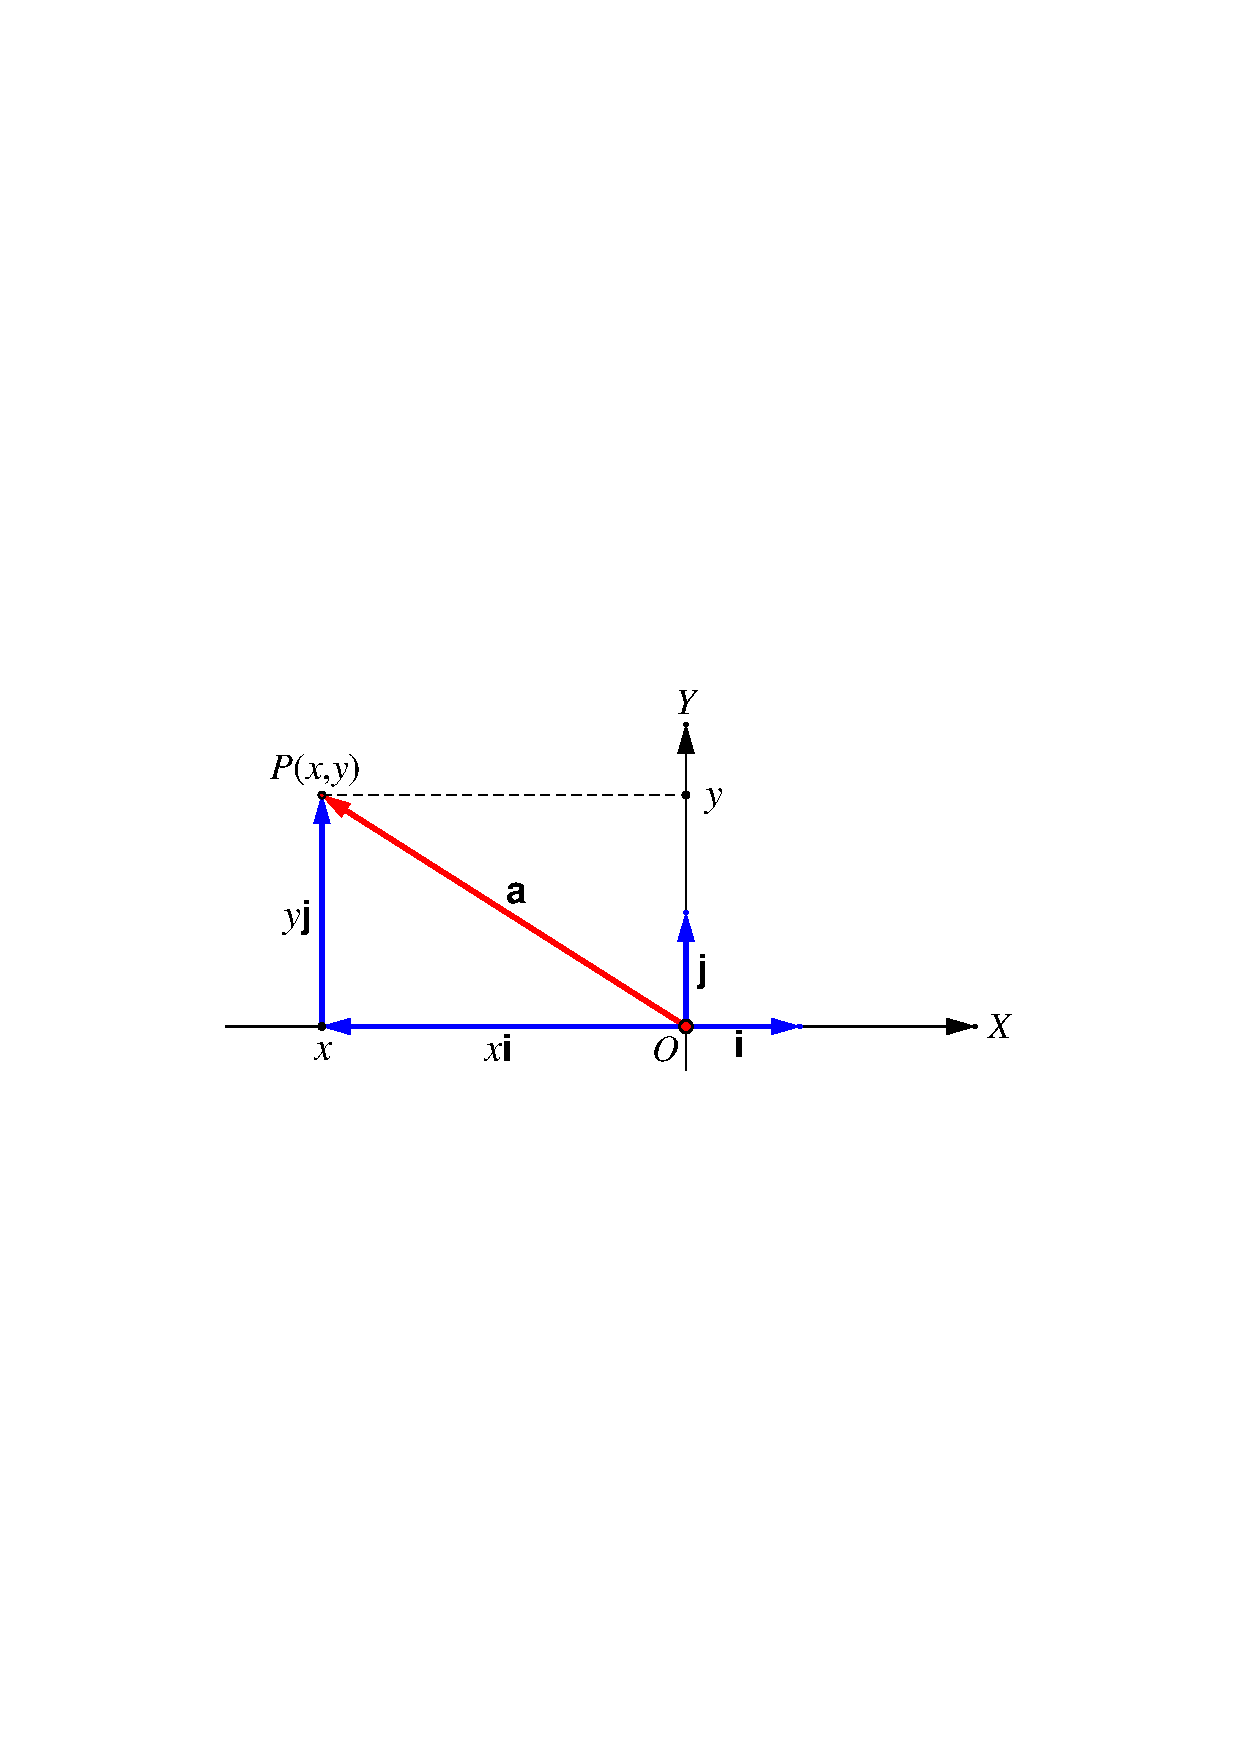
\includegraphics[trim=4cm 11.2cm 3.8cm 11.6cm,width=0.4\textwidth,clip]{geometer/vektor10c.pdf}		
		\\Figur 6.16		
\end{center}
På figuren er der i et $(O,\mathbf i,\mathbf j)$-koordinatsystem afsat en vilkårlig vektor $\mathbf a =\stackrel{\rightarrow}{OP}$. Da $\mathbf a = x\mathbf i + y\mathbf j$, og da $|x\mathbf i|=|x|$ og $|y\mathbf j|=|y|$, ser vi at koordinaterne for $\mathbf a$ med hensyn til e-basis er identiske med koordinaterne for punktet $P$, endepunktet for $\mathbf a$'s stedvektor. Et punkt har kort sagt de samme koordinater som dets tilhørende stedvektor.
\end{remark}

Indføringen af sædvanlig ortonormal basis og koordinater for vektorer i rummet foregår som en simpel udvidelse af den tilsvarende i planen. 

\begin{definition}[Standardbasis i rummet]
Ved en \ind{standardbasis}{standardbasis} eller en \ind{e-basis}{e-basis} for de geometriske vektorer i rummet forstås et ordnet sæt af tre vektorer $(\mathbf i,\mathbf j,\mathbf k)$ som opfylder:
\begin{itemize}
\item
$\mathbf i$, $\mathbf j$ og $\mathbf k$ har alle længden 1.
\item
$\mathbf i$, $\mathbf j$ og $\mathbf k$ er parvist ortogonale.
\item
Når $\mathbf i$, $\mathbf j$ og $\mathbf k$ afsættes ud fra origo, og når vi betragter $\mathbf i$ og $\mathbf j$ fra endepunktet af $\mathbf k$, så
overgår $\mathbf i$ i $\mathbf j$, når $\mathbf i$ drejes omkring origo med vinklen $\frac \pi 2$ mod uret.
\end{itemize}
Når $(\mathbf i,\mathbf j,\mathbf k)$ er en e-basis, forstås ved et $(O,\mathbf i,\mathbf j,\mathbf k)$-koordinatsystem et sædvanligt retvinklet $(X,Y,Z)$-koordinatsystem hvor $X$-aksen har origo som startpunkt og $\mathbf i$ som retningsvektor, $Y$-aksen har origo som startpunkt og $\mathbf j$ som retningsvektor, og $Z$-aksen har origo som startpunkt og $\mathbf k$ som retningsvektor.
\begin{center}
		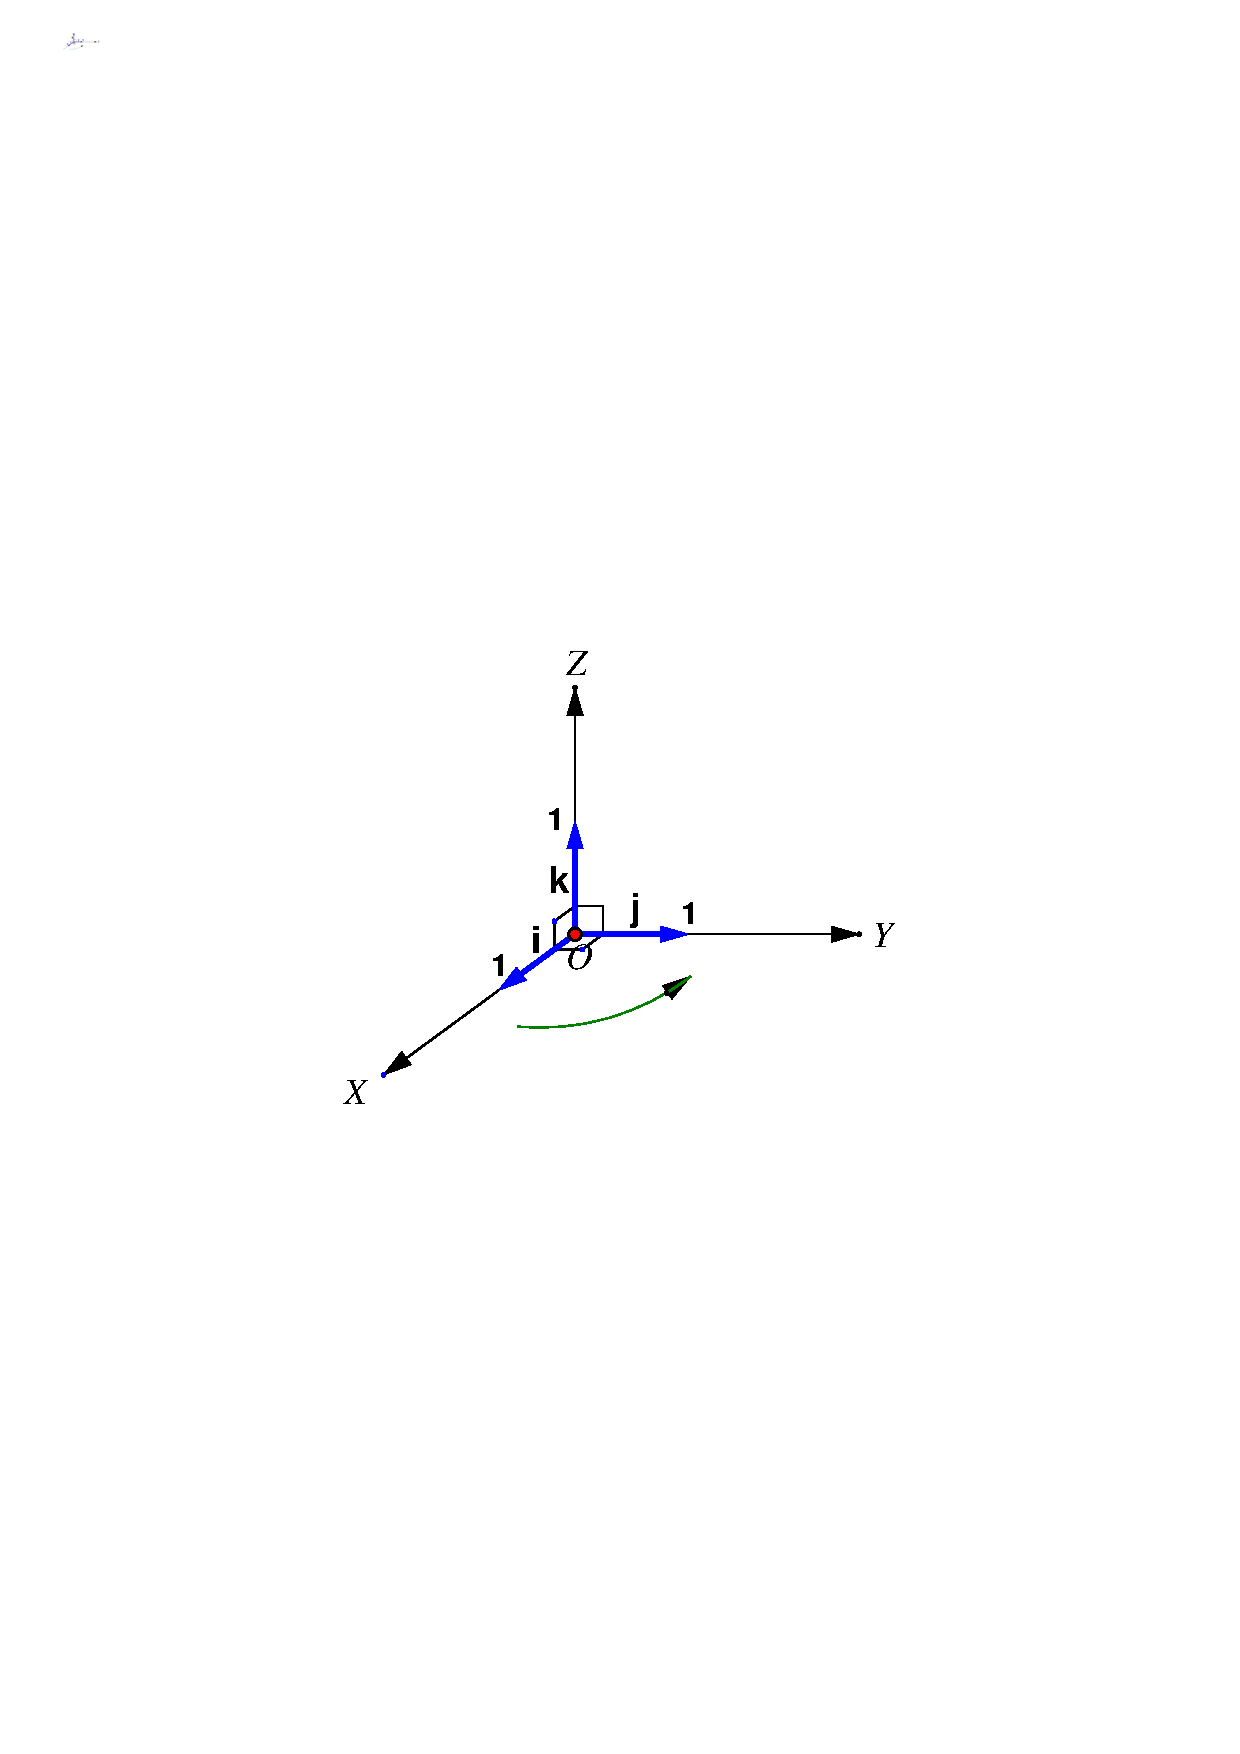
\includegraphics[trim=4cm 10.5cm 4cm 10.5cm,width=0.5\textwidth,clip]{geometer/vektor11.pdf}				
		\\Figur 6.17: Sædvanligt retvinklet koordinatsystem i rummet
\end{center}
\end{definition}

\begin{theorem}[En vektors $e$-koordinater]
Når $(\mathbf i,\mathbf j,\mathbf k)$ er en e-basis, kan enhver vektor $\mathbf v$ i rummet på netop én måde skrives som en linearkombination af $\mathbf i$, $\mathbf j$ og $\mathbf k$:
$$\mathbf v=x\mathbf i+y\mathbf j +z\mathbf k.$$
Koefficienterne $x$, $y$ og $z$ i linearkombinationen kaldes for $\mathbf v$'s \textit{koordinater med hensyn til e-basis}, eller kortere $\mathbf v$'s e-koordinater, og de samles i en \ind{koordinatvektor}{koordinatvektor} med følgende skrivemåde:
$$_\mathrm e\mathbf v=
\begin{matr}{r}x\\y\\z\end{matr}\,.$$
\end{theorem}

\begin{remark}[Et punkts koordinater]
\begin{center}
		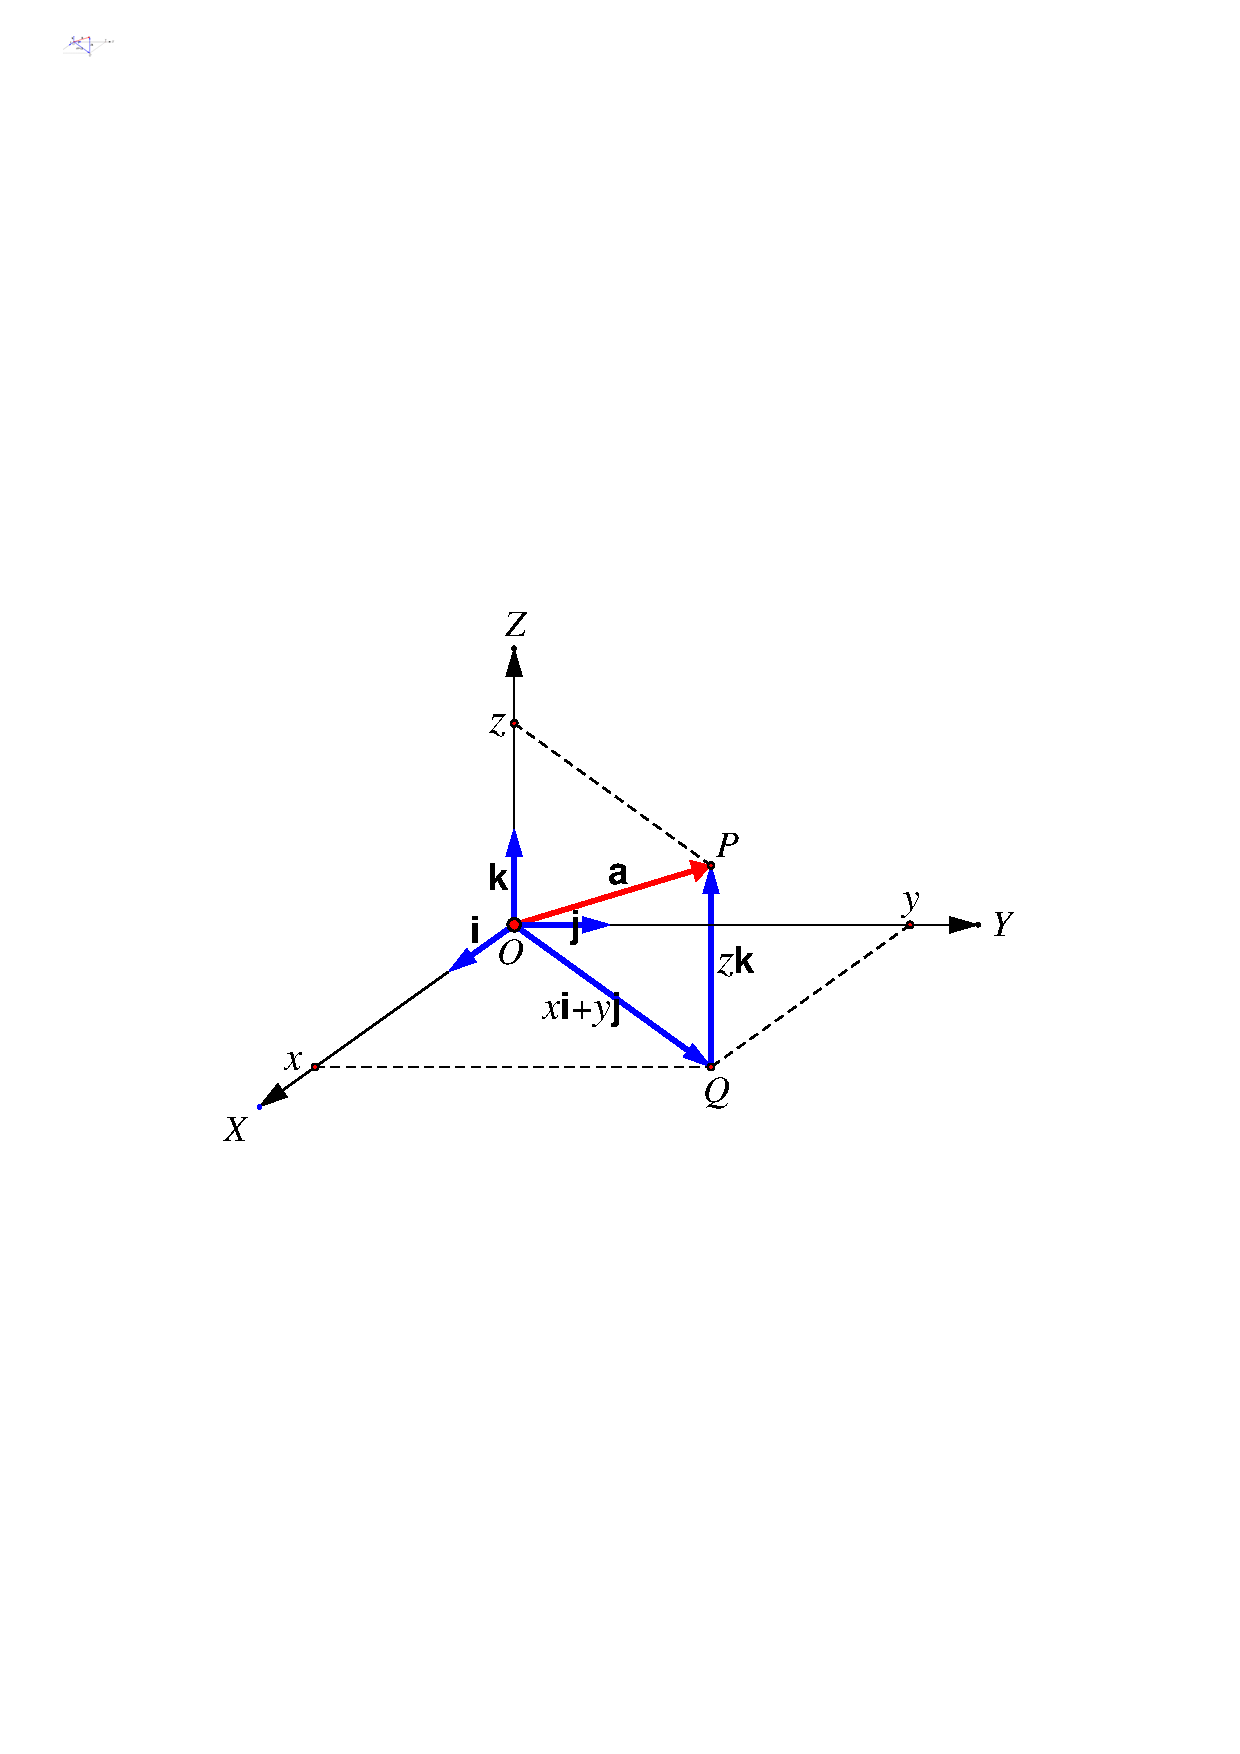
\includegraphics[trim=3cm 10cm 3cm 10cm,width=0.60\textwidth,clip]{geometer/vektor12.pdf}				
		\\Figur 6.18
\end{center}
På figuren er der i et $(O,\mathbf i,\mathbf j,\mathbf k)$-koordinatsystem afsat en vilkårlig vektor $\mathbf a =\stackrel{\rightarrow}{OP}$. Da $\mathbf a = \stackrel{\rightarrow}{OQ}+\stackrel{\rightarrow}{QP}=x\mathbf i + y\mathbf j+z\mathbf k$, og da $|x\mathbf i|=|x|$, $|y\mathbf j|=|y|$ og $|z\mathbf j|=|z|$, ser vi at koordinaterne for $\mathbf a$ med hensyn til e-basis er identiske med koordinaterne for punktet $P$, endepunktet for $\mathbf a$'s stedvektor. Et punkt har kort sagt de samme koordinater som dets tilhørende stedvektor.
\end{remark}
\section{Vilkårlige baser i planen og rummet}
Hvis der i planen er givet to lineært uafhængige vektorer, er det muligt at skrive enhver anden vektor i planen som en linearkombination af de to givne vektorer. På figur 6.19 betragter vi som eksempel de to lineært uafhængige vektorer $\mathbf a_1$ og $\mathbf a_2$ samt to andre vektorer $\mathbf u$ og $\mathbf v$:

\begin{center}
		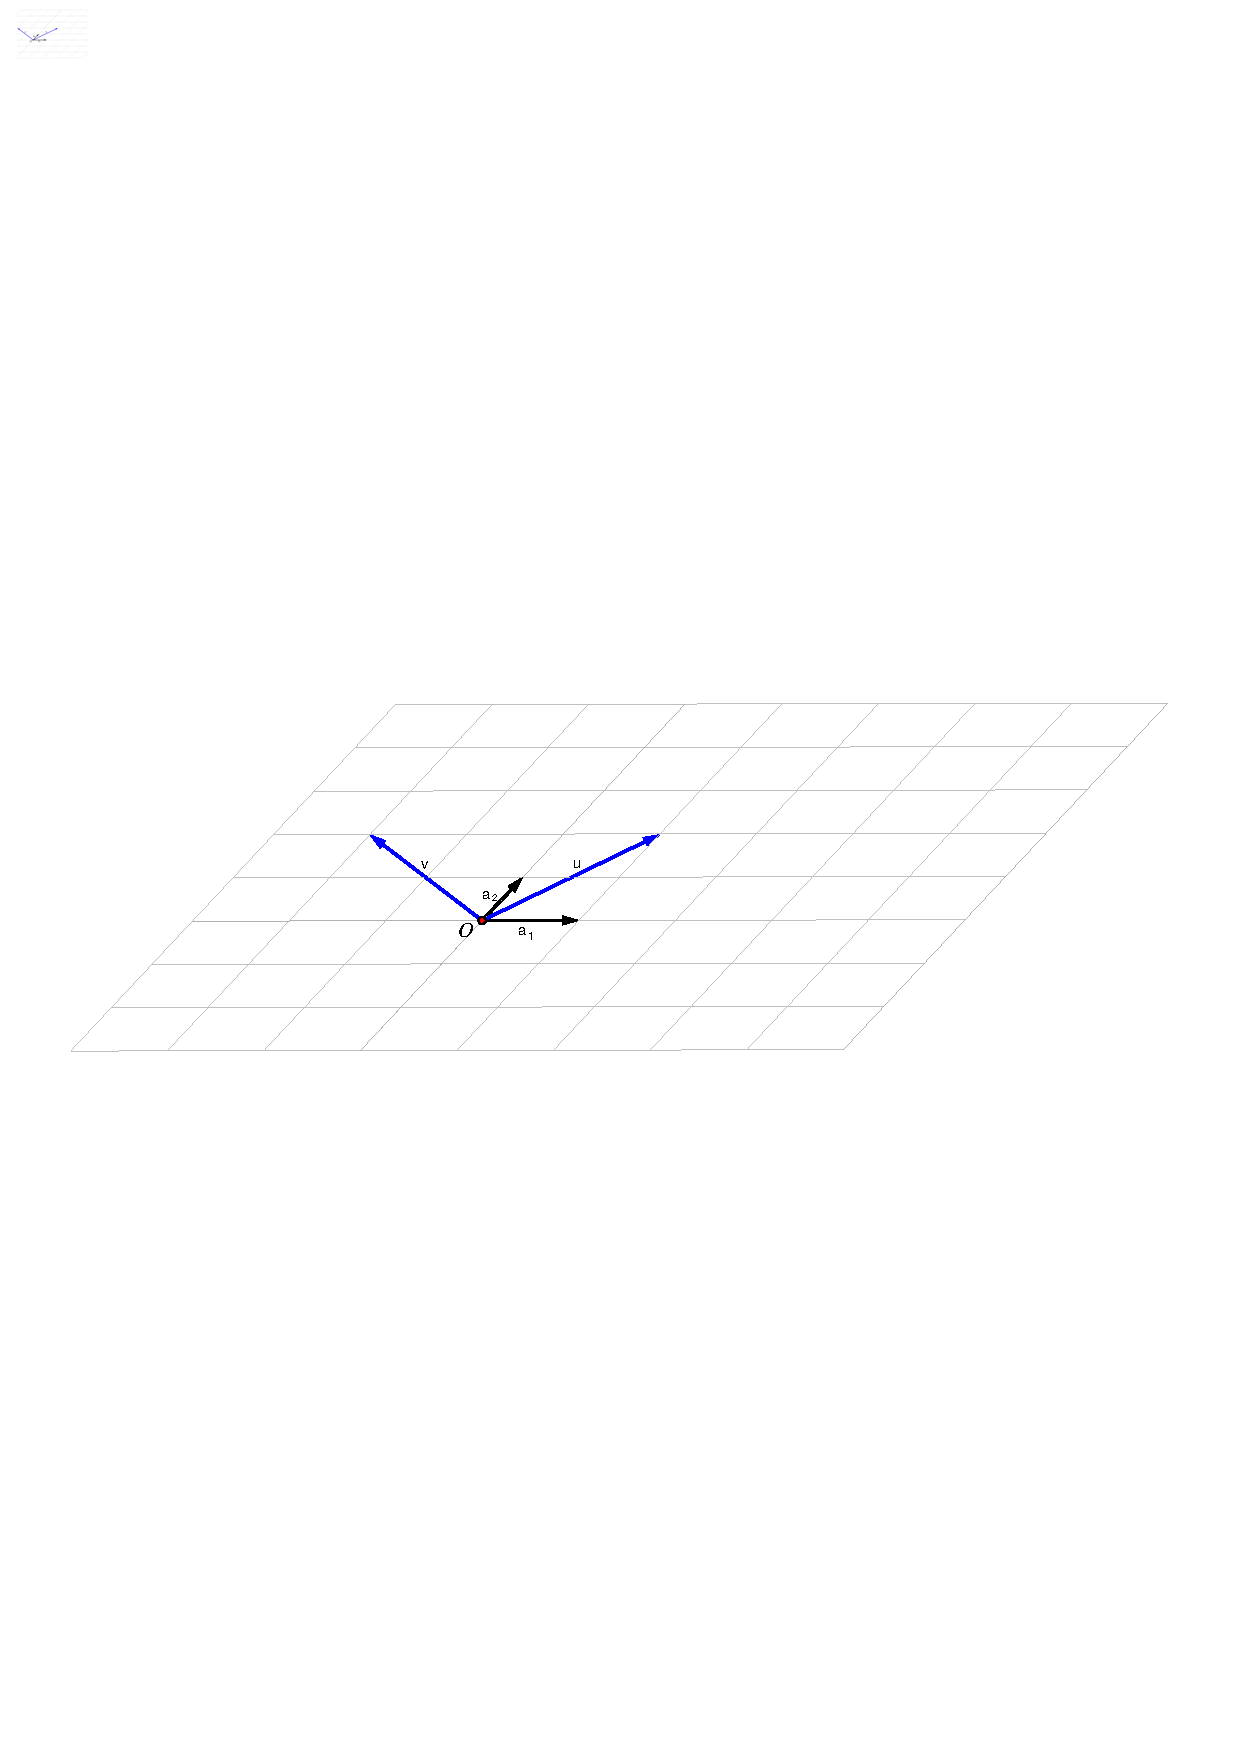
\includegraphics[trim=4cm 13cm 7.5cm 13.5cm,width=0.75\textwidth,clip]{geometer/abasis00ny.pdf}	
		\\Figur 6.19: Koordinatsystem i planen med basis $(\ma_1,\ma_2)$			
\end{center}
Vi ser at $\,\mathbf u=1\mathbf a_1+2\mathbf a_2\,$ og $\,\mathbf v=-2\mathbf a_1+2\mathbf a_2\,$. Disse linearkombinationer er entydige, idet $\mathbf u$ og $\mathbf v$ ikke kan skrives som linearkombination af $\mathbf a_1$ og $\mathbf a_2$ ved at benytte andre koefficienter end dem der her indgår. Enhver anden vektor i planen kan på tilsvarende vis skrives som en linearkombination af $\mathbf a_1$ og $\mathbf a_2$, man siger at de to vektorer \ind{udspænding}{udspænder} hele planen.\\

Dette gør det muligt at generalisere begrebet basis. I stedet for en standard e-basis kan vi vælge at benytte vektorsættet $(\mathbf a_1,\ma_2)$ som en basis for  vektorerne i planen, og vi kalder i så fald koefficenterne i linearkombinationerne ovenfor for \textit{koordinaterne} for $\mathbf u$ henholdsvis  $\mathbf v$ \textit{med hensyn til basen} a hvilket skrives således:
\begin{equation}
 _\mathrm a\mathbf u=
\begin{matr}{r}1\\2\end{matr}\,\,\mathrm{og}\,\,
 {_\mathrm a\mathbf v}=
\begin{matr}{r}-2\\2\end{matr}\,.
\end{equation}  
\smallskip\\ 
For mængden af geometriske vektorer i rummet går vi frem på tilsvarende måde. Er der givet tre lineært uafhængige vektorer, kan enhver vektor i rummet på entydig vis skrives som en linearkombination af de tre givne vektorer. De \textit{udspænder} hele rummet. Vi kan derfor vælge de tre vektorer som en basis for rumvektorerne, og udtrykke en vilkårlig rumvektor ved hjælp af koordinater med hensyn til denne basis. En fremgangsmåde til at bestemme koordinaterne er vist på figur 6.20, hvor der er givet en a-basis $(\mathbf a_1,\mathbf a_2,\ma_3)$ samt en vilkårlig vektor $\mathbf u$.
\begin{center}
		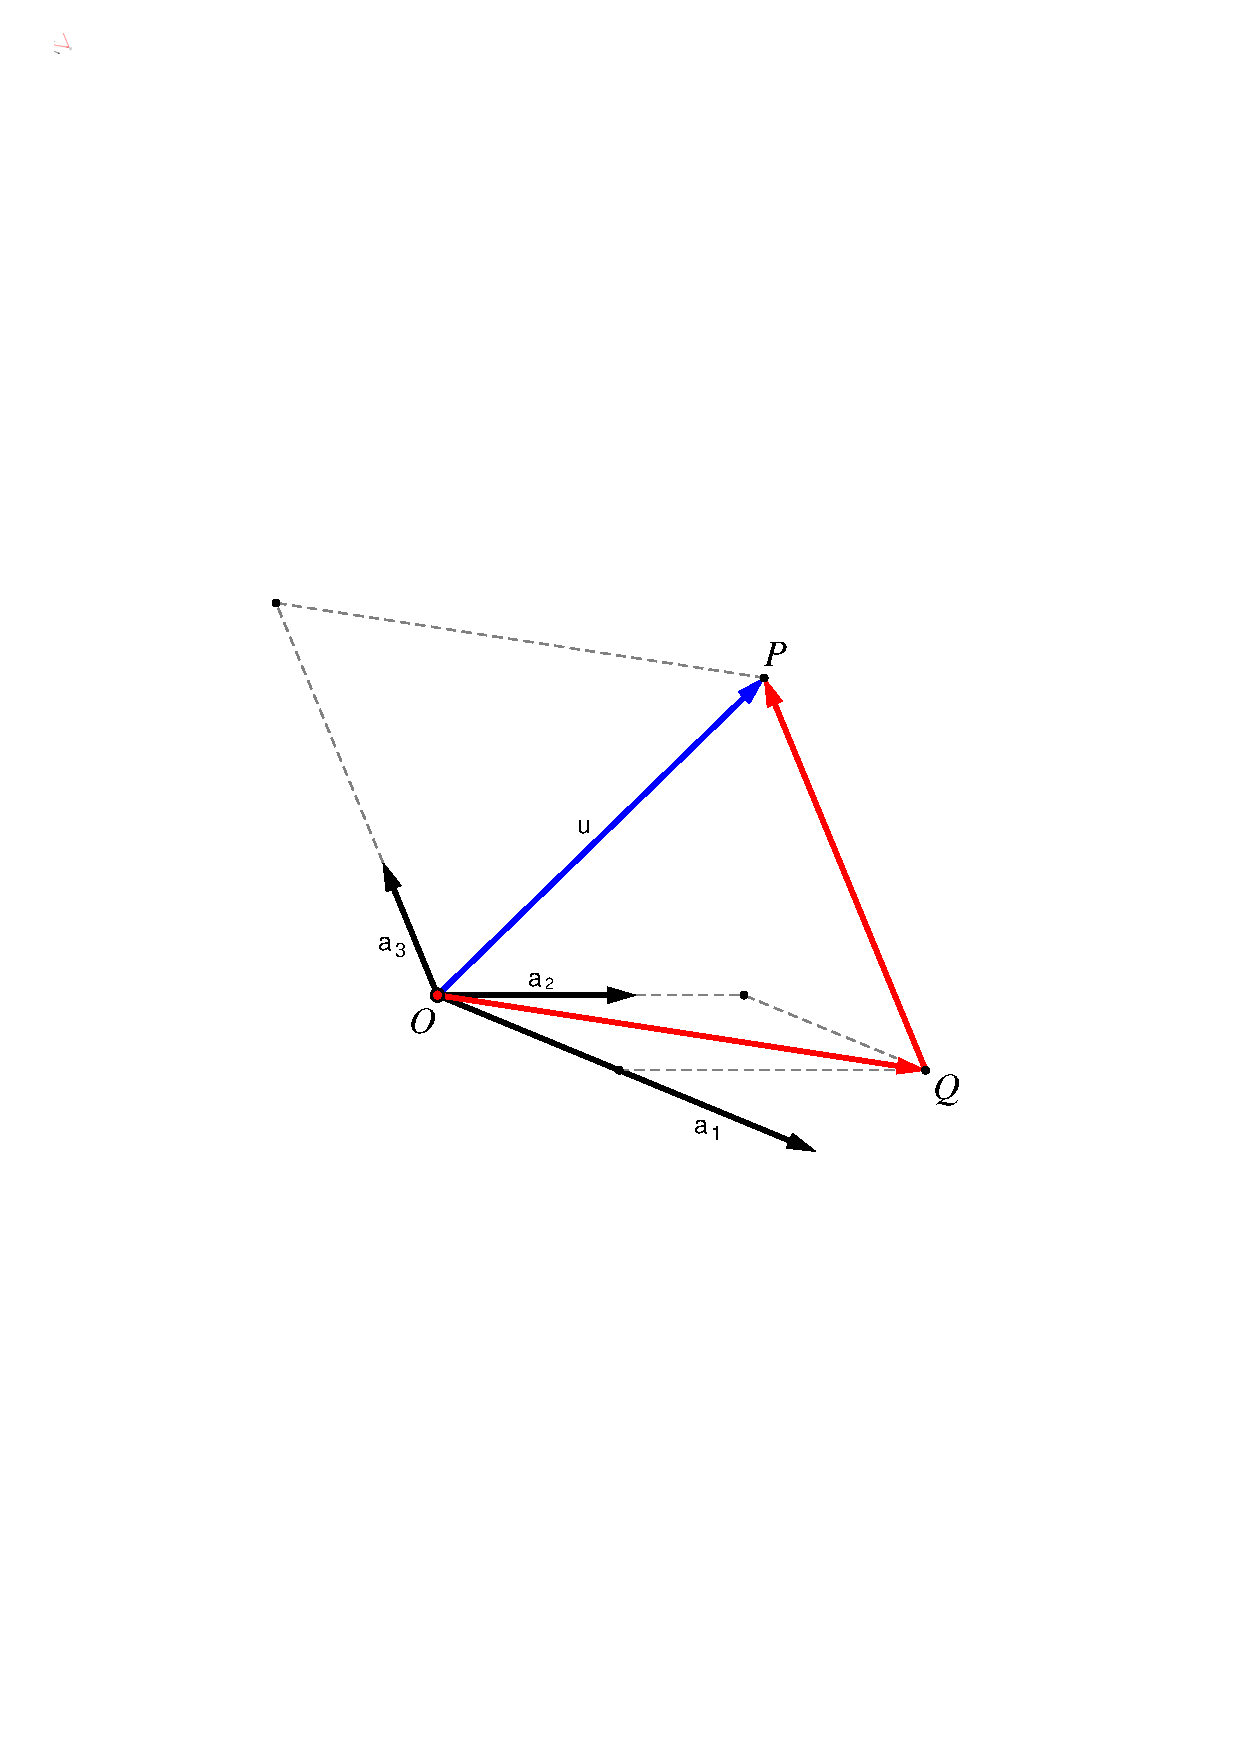
\includegraphics[trim=3cm 10cm 3cm 10cm,width=0.60\textwidth,clip]{geometer/abasis04.pdf}				
		\\Figur 6.20: Koordinatsystem med basis $(\ma_1,\ma_2,\ma_3)$
\end{center}
Gennem endepunktet $P$ for $\mathbf u$ trækkes en linje som er parallel med $\ma_3$, og det punkt hvor denne linje skærer den plan der indeholder $\ma_1$ og $\ma_2$, betegnes $Q$. Der findes da to tal $k_1$ og $k_2$ så $\stackrel{\rightarrow}{OQ}=k_1\ma_1+k_2\ma_2\,$ fordi $(\ma_1,\ma_2)$ udgør en basis i den plan som indeholder $\ma_1$ og $\ma_2\,$. Endvidere findes der et tal  $k_3$, så $\stackrel{\rightarrow}{QP}=k_3\ma_3$ da $\stackrel{\rightarrow}{QP}$ og $\ma_3$ er parallelle. Men så har vi
$$\mathbf u=\stackrel{\rightarrow}{OQ}+\stackrel{\rightarrow}{QP}=k_1\ma_1+k_2\ma_2+k_3\ma_3.
$$
$\mathbf u$ har dermed koordinatsættet $(k_1,k_2,k_3)$ med hensyn til basis $a$. 
\begin{example}[Koordinater med hensyn til en vilkårlig basis]\label{koordValgtBasis}
I rummet er der givet tre lineært uafhængige vektorer $\mathbf a_1,\mathbf a_2$ og $\mathbf a_3$ som vist på figur 6.21.
\begin{center}
		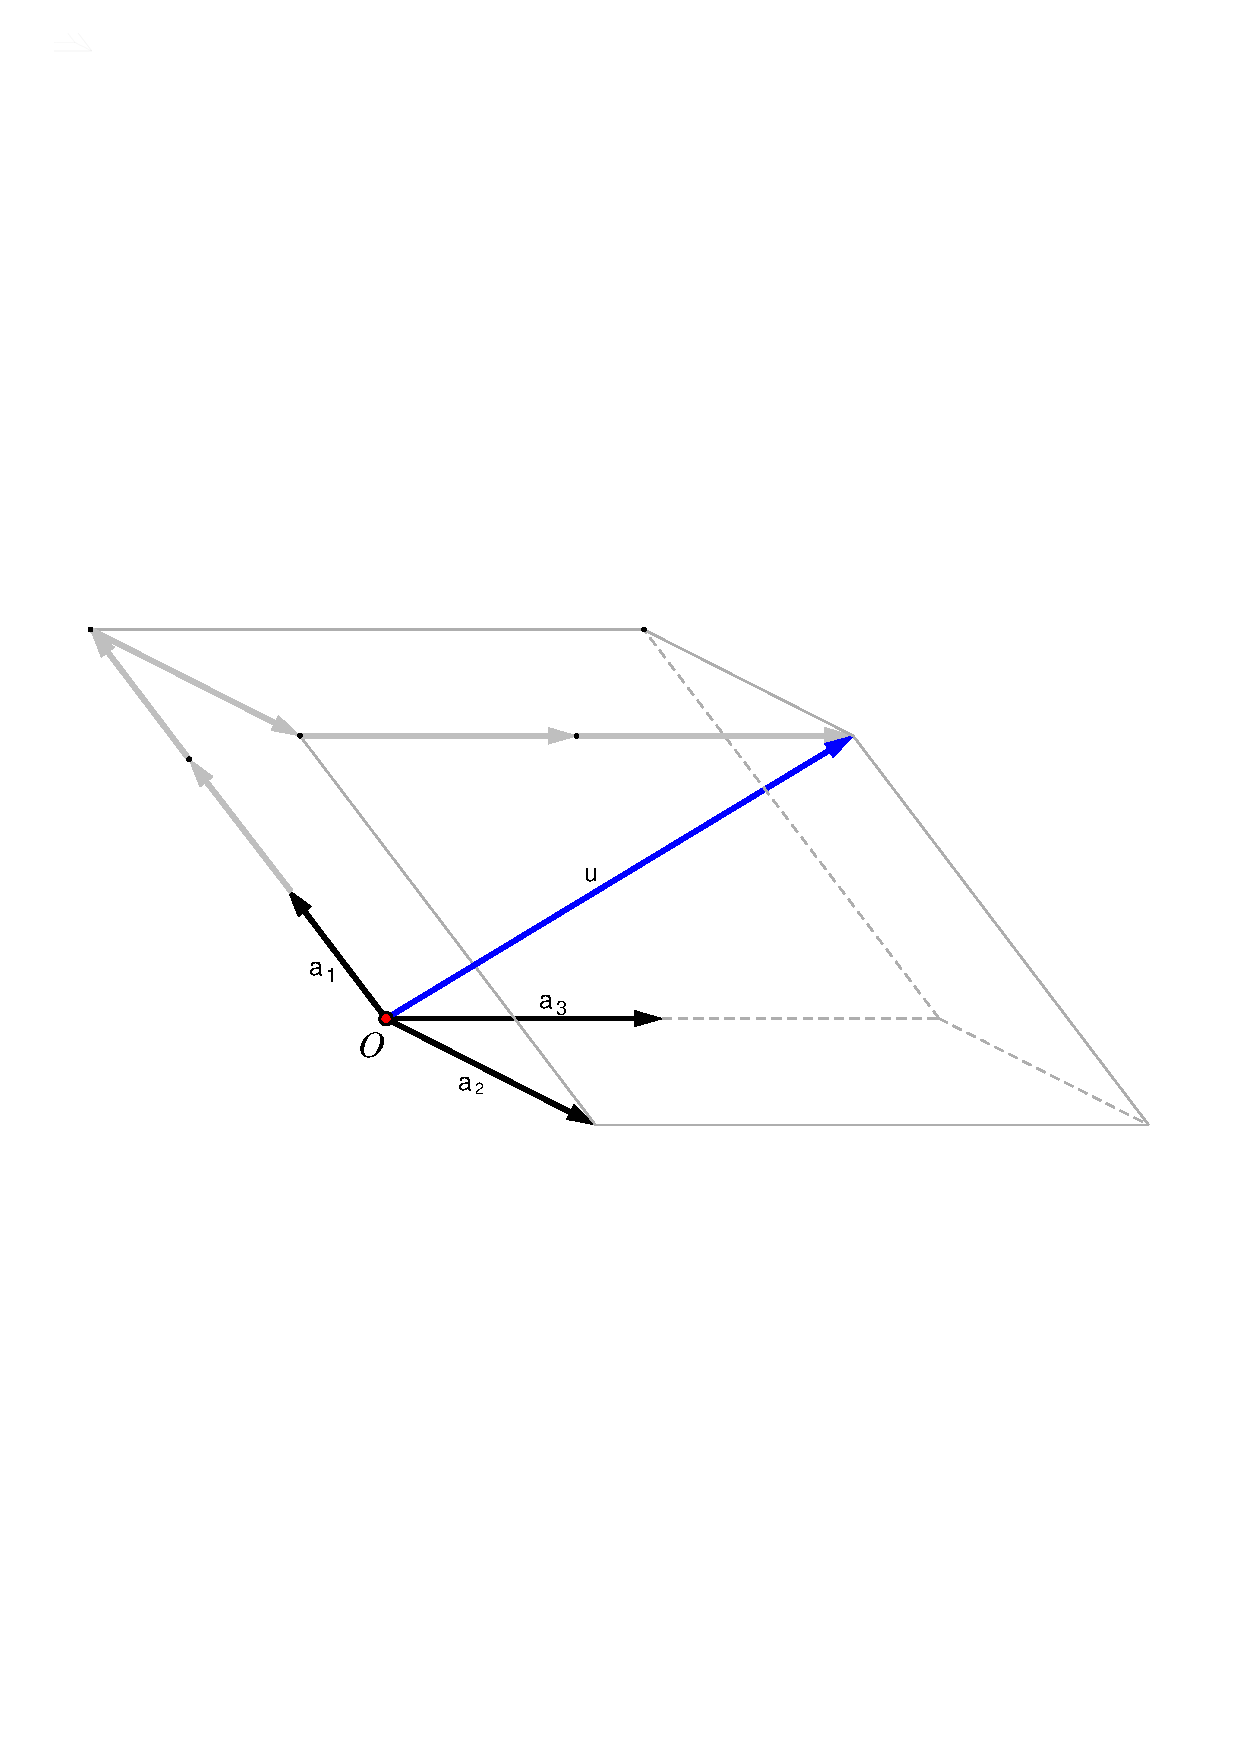
\includegraphics[trim=1cm 10cm 1cm 10cm,width=0.60\textwidth,clip]{geometer/abasis01b.pdf}				
		\\Figur 6.21: Koordinatsystem med basis $(\ma_1,\ma_2,\ma_3)$
\end{center}
Da $\mathbf u$ kan skrives som en linearkombination af $\mathbf a_1,\mathbf a_2$ og $\mathbf a_3$ på følgende måde
\begin{equation}
\mathbf u=3\mathbf a_1,+\mathbf a_2+2\mathbf a_3\,,
\end{equation}
så har $\mathbf u $ koordinaterne $(3,1,2)$ med hensyn til basen a givet ved $(\mathbf a_1,\mathbf a_2,\mathbf a_3)$ hvilket kort skrives således
\begin{equation}
 _\mathrm a\mathbf u=
\begin{matr}{r}3\\1\\2\end{matr}\,.
\end{equation}
\end{example}

Vi samler overvejelserne om vilkårlige baser ovenfor i den følgende mere formelle defintion:

\begin{definition}[Vektorers koordinater med hensyn til en basis]
\begin{itemize}
\item
Ved en basis \textit{a} for de geometriske vektorer i planen forstås et vilkårligt ordnet sæt af to lineært uafhængige vektorer $(\mathbf a_1,\mathbf a_2)$. Lad en vilkårlig vektor $\mathbf u$ være bestemt ved linearkombinationen $\mathbf u=x\mathbf a_1+y\mathbf a_2$. Koefficienterne $x$ og $y$ kaldes for $\mathbf u$'s \textit{koordinater med hensyn til basis a}, eller kortere $\mathbf u$'s a-koordinater, og de samles i en \textit{koordinatvektor} med følgende skrivemåde:
\begin{equation}
_\mathrm a\mathbf u=
\begin{matr}{r}x\\y\end{matr}\,.
\end{equation}
\item
Ved en basis \textit{b} for de geometriske vektorer i rummet forstås et vilkårligt ordnet sæt af tre lineært uafhængige vektorer $(\mathbf b_1,\mathbf b_2,\mathbf b_3)$. Lad en vilkårlig vektor $\mathbf v$ være bestemt ved linearkombinationen $\mathbf v=x\mathbf b_1+y\mathbf b_2+z\mathbf b_3$. Koefficienterne $x$, $y$ og $z$ kaldes for $\mathbf v$'s \textit{koordinater med hensyn til basis b}, eller kortere $\mathbf v$'s b-koordinater, og de samles i en \textit{koordinatvektor} med følgende skrivemåde:
\begin{equation}
_\mathrm b \mathbf v=
\begin{matr}{r}x\\y\\z \end{matr}\,.
\end{equation}
\end{itemize}
\end{definition}

En given vektors koordinatsæt ændres når man skifter valgt basis. Denne afgørende pointe tager vi hul på i den følgende opgave.

\begin{exercise}\label{tn6.basisskifte}
\begin{center}
		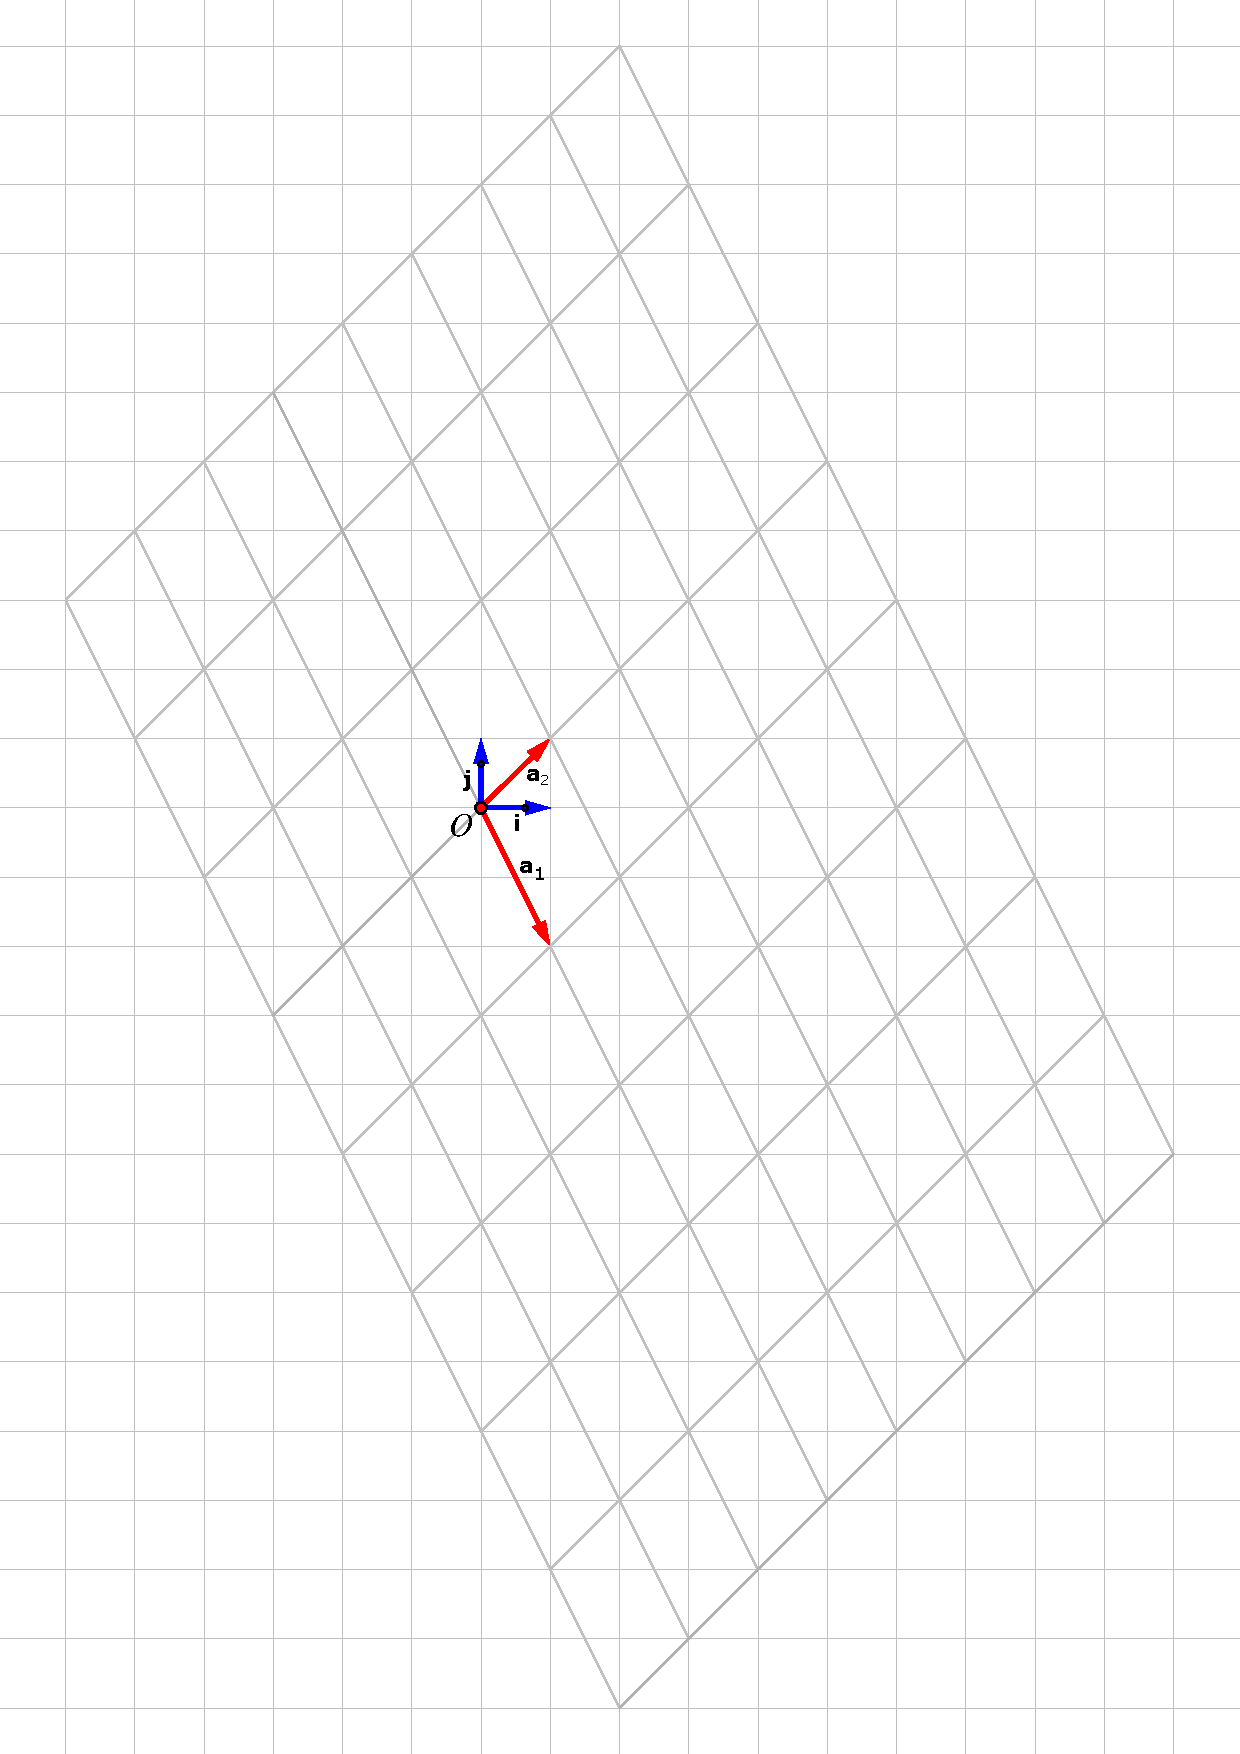
\includegraphics[trim=3cm 11.4cm 4.5cm 10cm,width=0.7,width=0.7\textwidth,clip]{geometer/abasis05.pdf}				
		\\Figur 6.22: Basisskifte
\end{center}
På figur 6.22 er der i planen givet standard e-basen $(\mathbf i, \mathbf j)$ samt en a-basis $(\mathbf a_1, \mathbf a_2)$.
\begin{enumerate}
\item
En vektor $\mathbf u$ har koordinaterne $(5,-1)$ med hensyn til e-basen. Bestem $\mathbf u$'s\\ a-koordinater.
\item
En vektor $\mathbf v$ har koordinaterne $(-1,-2)$ med hensyn til a-basen. Bestem $\mathbf v$'s\\ e-koordinater.
\end{enumerate}
\end{exercise} 
\begin{exercise}

\begin{center}
		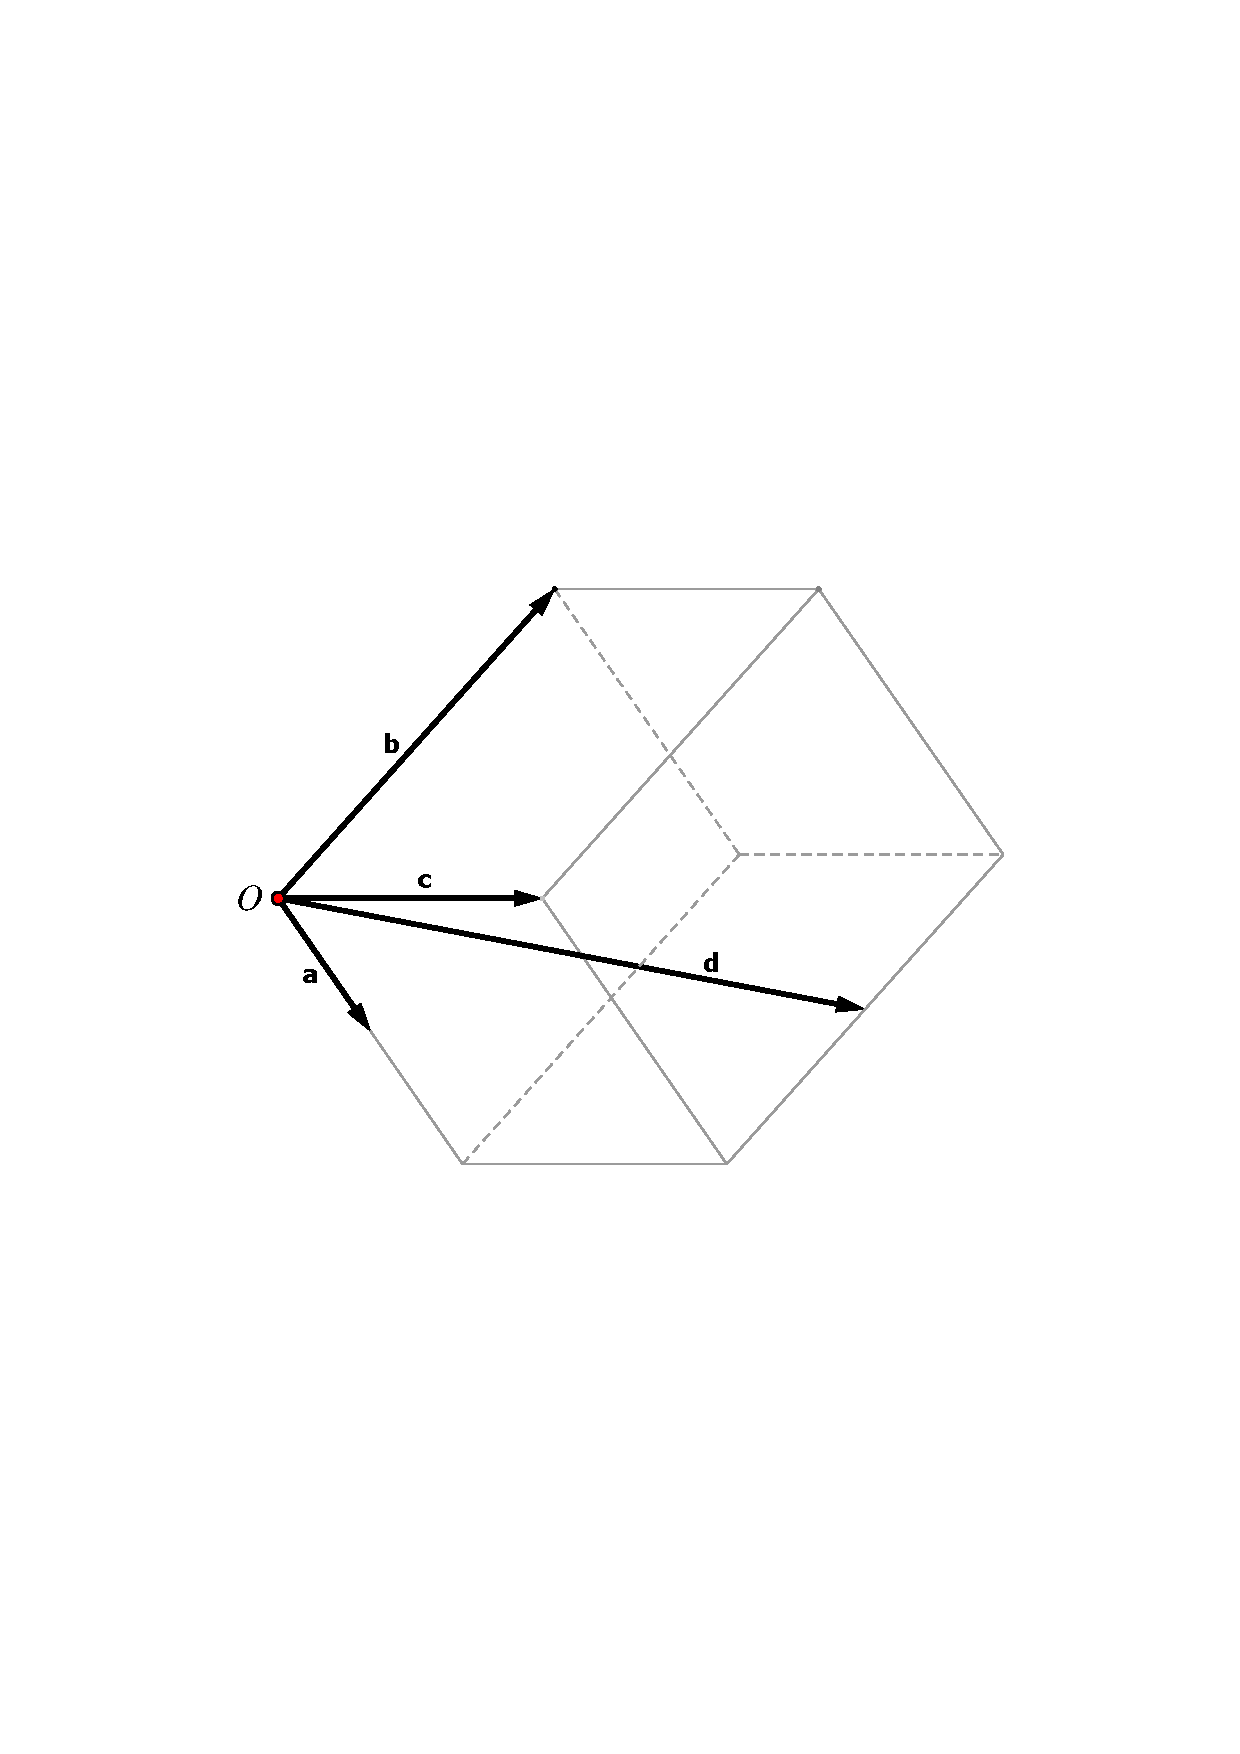
\includegraphics[trim=3cm 9.9cm 3cm 9.9cm,width=0.60\textwidth,clip]{geometer/abasis02.pdf}				
		\\Figur 6.23
\end{center}
\begin{enumerate}
\item
Det fremgår af figur 6.23, at $\mathbf a$, $\mathbf b$ og $\mc$ er lineært uafhængige. En basis m er derfor givet ved $(\mathbf a, \mathbf b,\mathbf c)$. Bestem koordinatvektoren $_\mathrm m\mathbf d$. 
\item 
Det fremgår også af figuren, at $(\mathbf a, \mathbf b,\mathbf d)$ er en basis, lad os kalde den n. Bestem koordinatvektoren $_\mathrm n\mathbf c$.
\item
Indtegn med origo som begyndelsespunkt den vektor $\mathbf u$ som har m-koordinaterne
$$
 _\mathrm m\mathbf u=
\begin{matr}{r}2\\1\\1\end{matr}\,.
$$
\end{enumerate}

\end{exercise}  

\section{Vektorregning ved hjælp af koordinater}
Når man har valgt en basis for de geometriske vektorer i planen (eller i rummet), så kan alle vektorer beskrives og fastlægges ved hjælp af deres koordinater med hensyn til den valgte basis. Til de to regneoperationer,  addition og multiplikation med skalar som tidligere er indført i denne eNote ved geometrisk konstruktion, får vi hermed et særdeles praktisk alternativ. I stedet for at udføre de geometriske regne-konstruktioner kan vi blot gennemføre taludregninger med de koordinater der svarer til den valgte basis.\\

Vi illustrerer dette med et eksempel fra planen hvor der er givet en basis a ved $(\mathbf a_1,\mathbf a_2)$ samt to vektorer $\mathbf u$ og $\mathbf v$ afsat ud fra $O$, se figur 6.24. Opgaven består i at bestemme vektoren $\mathbf b = 2\mathbf u-\mathbf v$, og vi vil gøre det på to forskellige metoder.

\begin{center}
		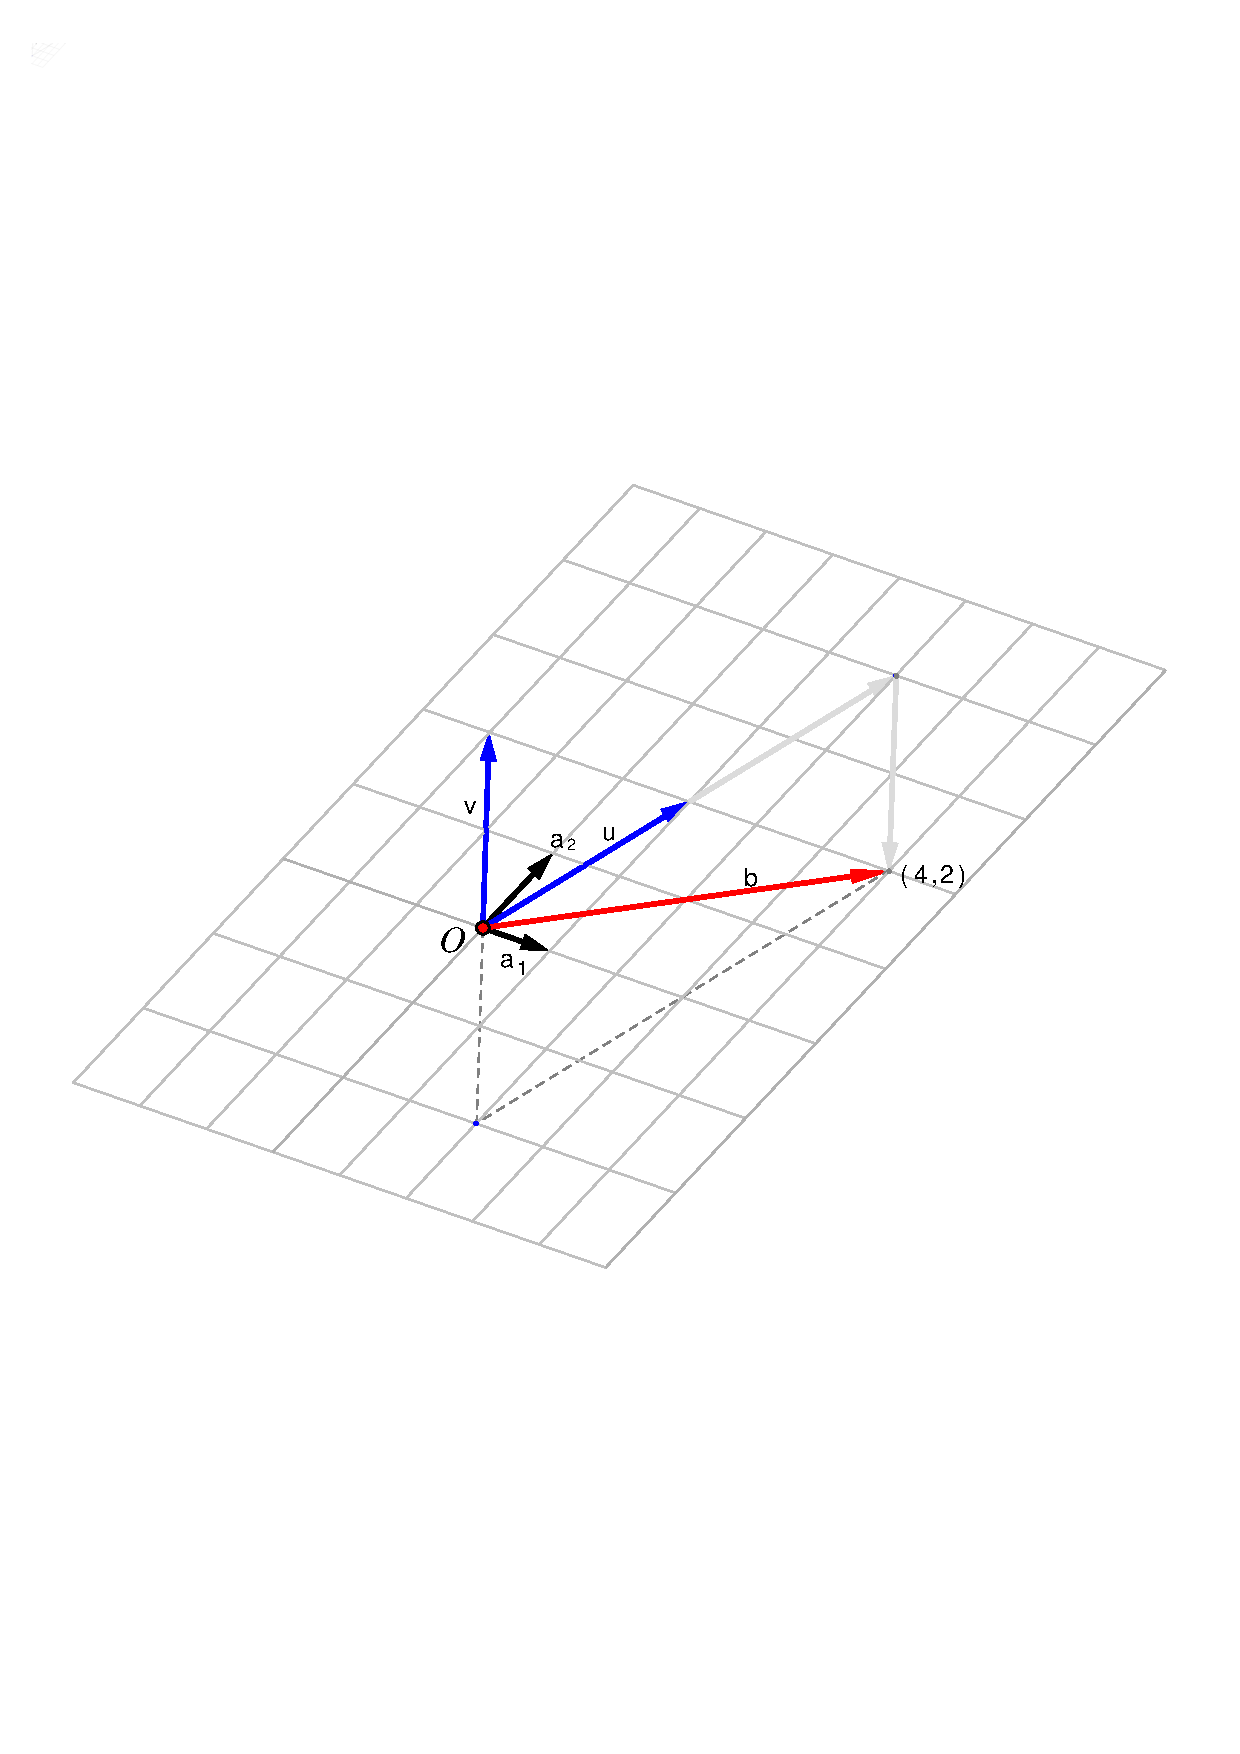
\includegraphics[trim=5.5cm 10cm 3.5cm 10cm,width=0.50\textwidth,clip]{geometer/abasis0b.pdf}	
		\\Figur 6.24: Linearkombination bestemt vha. koordinater			
\end{center}
Metode 1 (geometrisk): Først udfører vi regneoperationerne som defineret i \ref{addition} og \ref{multiplikation}, jævnfør de grå hjælpevektorer i figur 6.24. \\

Metode 2 (algebraisk): Vi aflæser koordinaterne for $\mathbf u$ og $\mathbf v$ og udfører regneoperationerne direkte på koordinaterne:
 \begin{equation}
_\mathrm a\mathbf b=2\,_\mathrm a\mathbf u-_\mathrm a\mathbf v=
2\begin{matr}{r}1\\2\end{matr}-\begin{matr}{r}-2\\2\end{matr}=
\begin{matr}{r}4\\2\end{matr}\,.
\end{equation} 
Herefter kan $\mathbf b$ tegnes direkte ud fra dens koordinater $(4,2) $ med hensyn til basen a.\\

At vi har ret til at følge denne fremgangsmåde fremgår af den følgende sætning.

\begin{theorem}[Grundlæggende koordinat-regneregler]\label{tn6.koord_linearitet}
I planen eller rummet er der givet to vektorer $\mathbf u$ og $\mathbf v$ samt et reelt tal $\,k\,$. Der er endvidere valgt en vilkårlig basis a. De to regneoperationer $\mathbf u + \mathbf v$ og $k\,\mathbf u$ kan da udføres ved hjælp af koordinater således:
\begin{enumerate}
\item
$_\mathrm a(\mathbf u+\mathbf v)={_\mathrm{a}\mathbf{u}}+{_\mathrm a\mathbf v}$
\item
$_\mathrm a(k\mathbf u)=k\,_\mathrm a\mathbf u$
\end{enumerate}

Sagt med ord: Koordinaterne for en vektorsum fås ved at lægge koordinaterne for addenderne sammen. Og koordinaterne for en vektor ganget med et tal er vektorens koordinater ganget med tallet. 
\end{theorem}\label{tn6.koordinater}
\begin{bevis}
Vi gennemfører beviset for mængden af de geometriske rumvektorer. Antag at koordinaterne for $\mathbf u$ og $\mathbf v$ med hensyn til den valgte basis a er givet ved
\begin{equation}
_\mathrm{a}\mathbf{u}=\begin{matr}{r}u_1\\u_2\\u_3\end{matr}
\,\,\mathrm{og}\,\,\,
_\mathrm{a}\mathbf{v}=\begin{matr}{r}v_1\\v_2\\v_3\end{matr}\,.
\end{equation}
Vi har da
\begin{equation}
\mathbf{u}=u_1\mathbf a_1+u_2\mathbf a_2+u_3\mathbf a_3
\,\,\mathrm{og}\,\,
\mathbf{v}=v_1\mathbf a_1+v_2\mathbf a_2+v_3\mathbf a_3
\end{equation}
og dermed i følge kommutativ, associativ og distributiv regneregel, se \ref{tn6.regneregler}
\begin{equation}
\begin{array}{c}
\mathbf{u}+\mathbf{v}=(u_1\mathbf a_1+u_2\mathbf a_2+u_3\mathbf a_3)+
(v_1\mathbf a_1+v_2\mathbf a_2+v_3\mathbf a_3)\\
=(u_1+v_1)\mathbf a_1+(u_2+v_2)\mathbf a_2+(u_3+v_3)\mathbf a_3
\end{array}
\end{equation}
hvilket medfører at
\begin{equation}
_\mathrm a(\mathbf u+\mathbf v)= \begin{matr}{r}u_1+v_1\\u_2+v_2\\u_3+v_3\end{matr}=
\begin{matr}{r}u_1\\u_2\\u_3\end{matr}
+\begin{matr}{r}v_1\\v_2\\v_3\end{matr}= {_\mathrm{a}\mathbf{u}}+{_\mathrm{a}\mathbf{v}}
\end{equation}
hvorefter første del af beviset er fuldført. Ved anden del af beviset benytter vi igen en distributiv regneregel, se \ref{tn6.regneregler}:\\
\begin{equation}
k\mathbf u=k(u_1\mathbf a_1+u_2\mathbf a_2+u_3\mathbf a_3)
=(k\cdot u_1)\mathbf a_1+(k\cdot u_2)\mathbf a_2+(k\cdot u_3)\mathbf a_3
\end{equation}
hvilket medfører at
\begin{equation}
_\mathrm a(k\mathbf u)=\begin{matr}{r}k\cdot u_1\\k\cdot u_2\\k\cdot u_1\end{matr}=
k\begin{matr}{r}u_1\\u_2\\u_3\end{matr}=k\,_\mathrm a\mathbf u
\end{equation}
hvorefter anden del af beviset er fuldført.
\end{bevis}
Sætning \ref{tn6.koordinater} gør det muligt at gennemføre mere komplicerede regneopgaver ved hjælp af koordinater, se det følgende eksempel. 
\begin{example}[Koordinatvektor for en linearkombination]
De tre plane vektorer $\mathbf a,\,\mathbf b$ og $\mathbf c$ har følgende koordinatvektorer med hensyn til en valgt basis v:
\begin{equation}
{_\mathrm{v}\mathbf{a}}=\begin{matr}{r}1\\2 \end{matr},\,
{_\mathrm{v}\mathbf{b}}=\begin{matr}{r}0\\1 \end{matr}\,\,\mathrm{og}\,\,\,
{_\mathrm{v}\mathbf{c}}=\begin{matr}{r}5\\-1 \end{matr}\,.
\end{equation}
\textit{Opgave}: Bestem koordinatvektoren for $\mathbf d=\mathbf a-2\mathbf b+3\mathbf c$ med hensyn til basis v.\\
\textit{Løsning}: 
\begin{align*}
%\begin{array}{c}
{_\mathrm{v}\mathbf{d}}&={_\mathrm{v}(\mathbf{a}-2\mathbf{b}+3\mathbf{c})}\\
&={_\mathrm{v}(\mathbf{a}+(-2)\mathbf{b}+3\mathbf{c})}\\
&={_\mathrm{v}\mathbf{a}}+{_\mathrm{v}(-2\mathbf{b})}+{_\mathrm{v}(3\mathbf{c})}\\
&={_\mathrm{v}\mathbf{a}}-2\,{_\mathrm{v}\mathbf{b}}+3\,{_\mathrm{v}\mathbf{c}}\\
&=\begin{matr}{r}1\\2 \end{matr}-2\begin{matr}{r}0\\1 \end{matr}+3\begin{matr}{r}5\\-1 \end{matr}=\begin{matr}{r}16\\-3 \end{matr}\,.
%\end{array}
\end{align*}
Her opnås det tredje lighedstegn ved første del af sætning \ref{tn6.koordinater} og det fjerde lighedstegn ved anden del af denne sætning.
\end{example}

\begin{example}[En plans parameterfremstilling i koordinater]\label{planParamKoord}
\begin{center}
		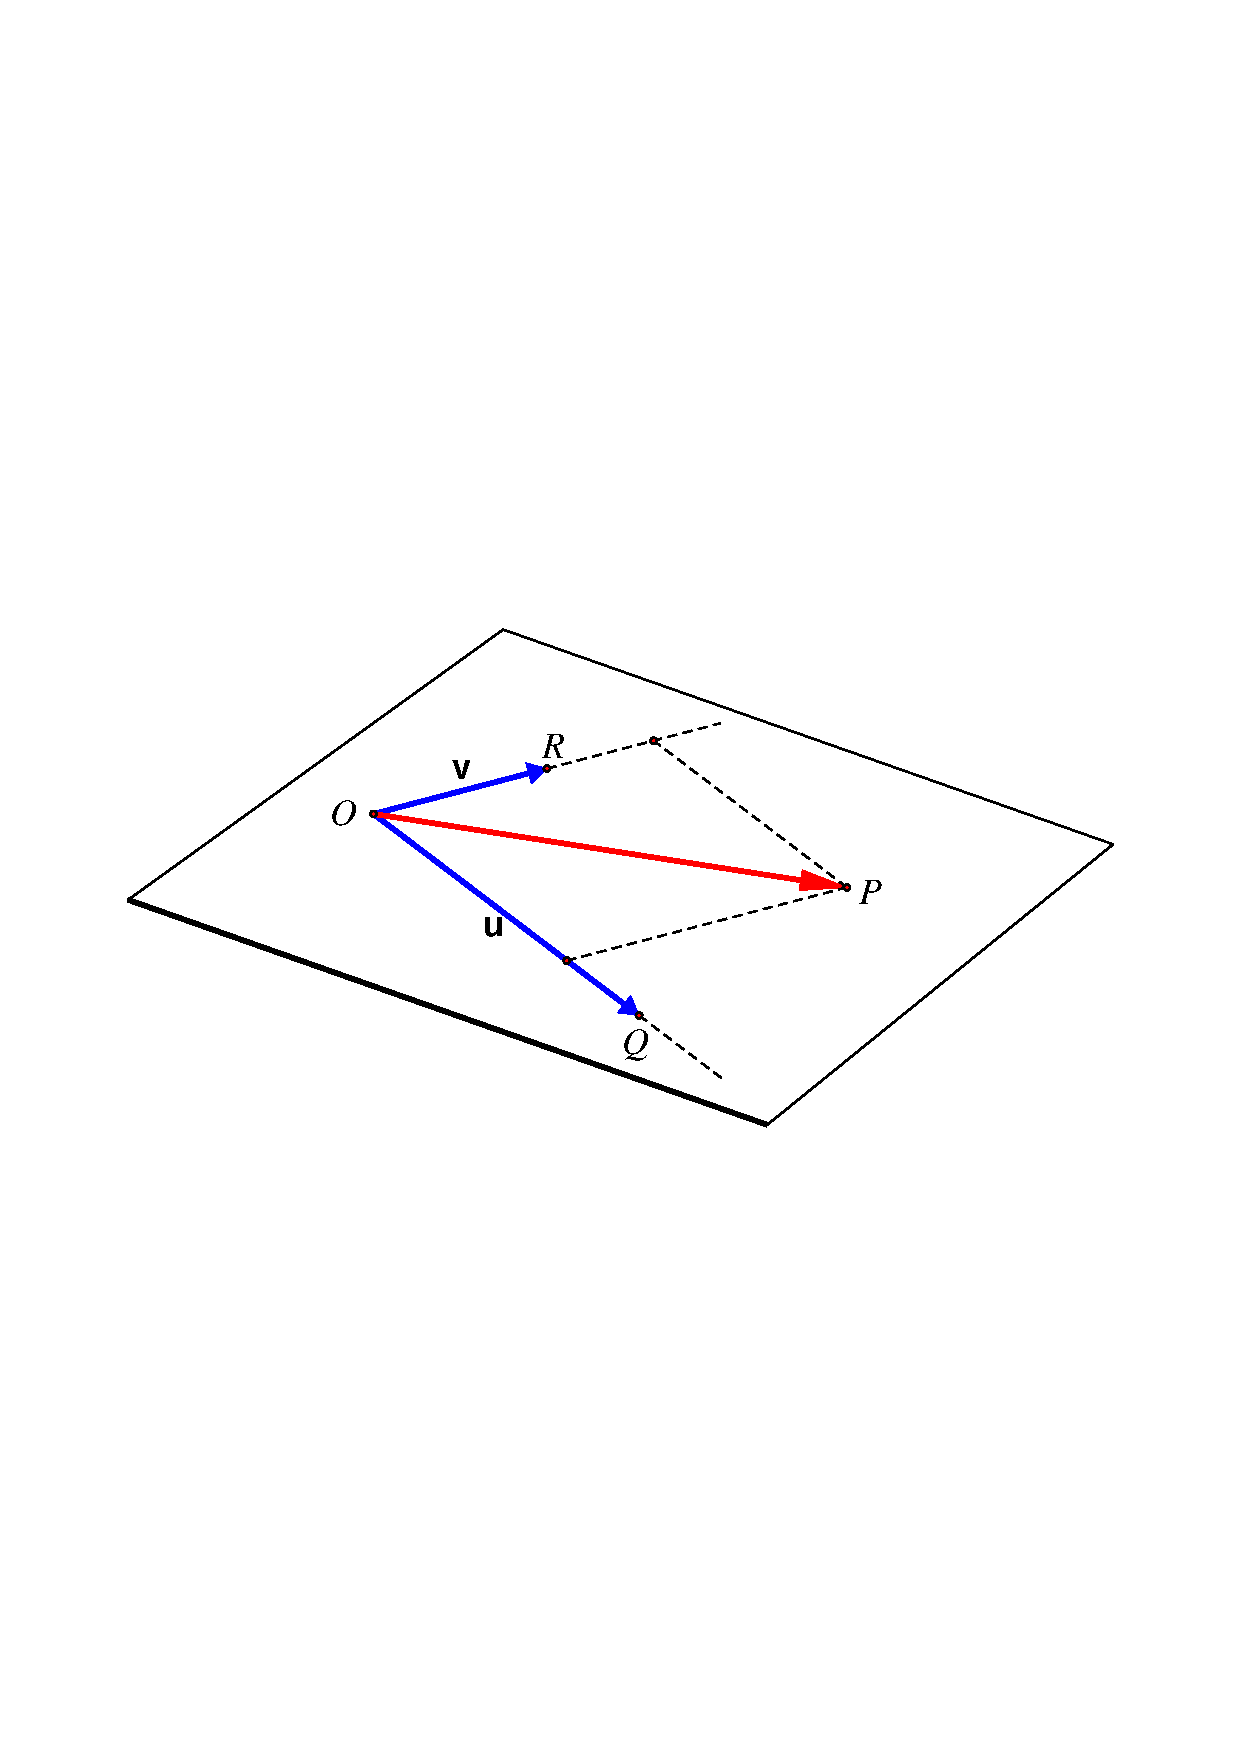
\includegraphics[trim=1.5cm 10.5cm 1.5cm
 10.7cm,width=0.60\textwidth,clip]{geometer/vektor14.pdf}	
   \\Figur 6.25: En plan i rummet	
\end{center}
Planen gennem origo som er vist på figur 6.25, har i følge eksempel \ref{tn6.planRum1} parameterfremstil\-lingen
\begin{equation}\label{tn6.PfPLan1}
\{P\,|\, \stackrel{\rightarrow}{OP}=s\mathbf u+t\mathbf v\,;\,\,(s,t)\in \mathbb R^2\}.
\end{equation}
Antag at der i rummet er givet en basis a og at
$$
{_\mathrm{a}\mathbf{u}}=\begin{matr}{r}u_1\\u_2\\u_3 \end{matr}\,\,\mathrm{og}\,\,\,
{_\mathrm{a}\mathbf{v}}=\begin{matr}{r}v_1\\v_2\\v_3 \end{matr}\,.
$$
Parameterfremstillingen (\ref{tn6.PfPLan1}) kan da skrives på koordinatform således:
\begin{equation}\label{tn6.PfPLanKoord1}
\begin{matr}{r}x\\y\\z \end{matr}=
s\begin{matr}{r}u_1\\u_2\\u_3 \end{matr}+
t\begin{matr}{r}v_1\\v_2\\v_3 \end{matr}
\end{equation}
hvor $\,_\mathrm{a}\hspace{-0.1cm}\stackrel{\rightarrow}{OP}=(x,y,z)$ og $(s,t)\in \mathbb R^2\,$.
\end{example}

\begin{example}[En plans parameterfremstilling i koordinater]
\begin{center}
		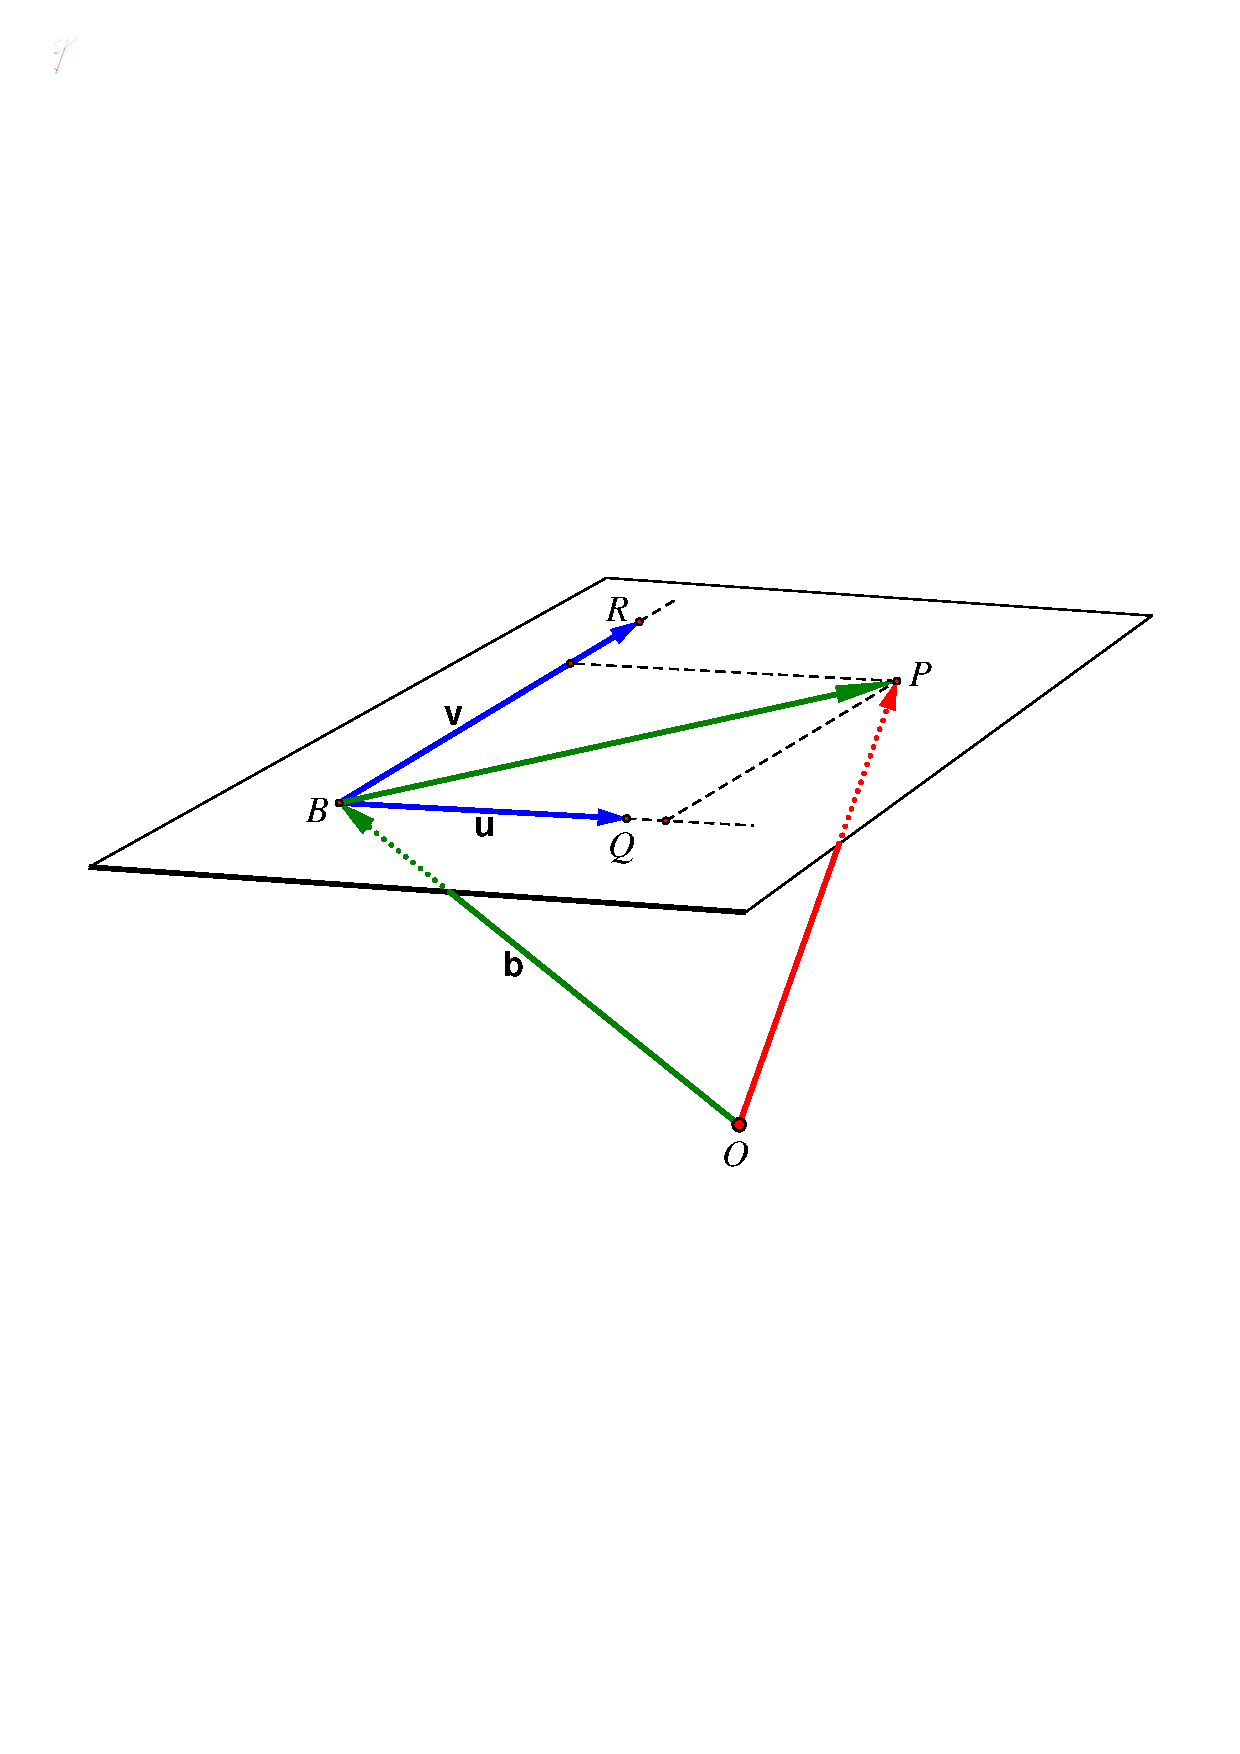
\includegraphics[trim=1.5cm 9.5cm 1.5cm
 9.5cm,width=0.65\textwidth,clip]{geometer/vektor15.pdf}	
   \\Figur 6.26: En plan i rummet	
\end{center}
Planen som er vist på figur 6.26, har i følge eksempel \ref{tn6.planRum2} parameterfremstillingen
\begin{equation}\label{tn6.PfPLan2}
\{P\,|\, \stackrel{\rightarrow}{OP}=\mb+s\mathbf u+t\mathbf v\,;\,\,(s,t)\in \mathbb R^2\}.
\end{equation}
Antag at der i rummet er givet en basis a og at
$$
{_\mathrm{a}\mathbf{b}}=\begin{matr}{r}b_1\\b_2\\b_3 \end{matr},\,
{_\mathrm{a}\mathbf{u}}=\begin{matr}{r}u_1\\u_2\\u_3 \end{matr}\,\,\mathrm{og}\,\,\,
{_\mathrm{a}\mathbf{v}}=\begin{matr}{r}v_1\\v_2\\v_3 \end{matr}\,.
$$
Parameterfremstillingen (\ref{tn6.PfPLan2}) kan da skrives på koordinatform således:
\begin{equation}\label{tn6.PfPLanKoord2}
\begin{matr}{r}x\\y\\z \end{matr}=
\begin{matr}{r}b_1\\b_2\\b_3 \end{matr}+
s\begin{matr}{r}u_1\\u_2\\u_3 \end{matr}+
t\begin{matr}{r}v_1\\v_2\\v_3 \end{matr}
\end{equation}
hvor $\,_\mathrm{a}\hspace{-0.1cm}\stackrel{\rightarrow}{OP}=(x,y,z)$ og $(s,t)\in \mathbb R^2\,$
\end{example}

\section{Vektorligninger og matrixalgebra}
En lang række problemer vedrørende vektorer fører til vektorligninger. Hvis vi ønsker at løse ligningerne ved hjælp af vektorernes koordinater med hensyn til en given basis, opstår der lineære ligningssystemer. Problemerne kan da løses ved hjælp af matrixmetoder der ligger i forlængelse af \tref{NUID1-tn2}{eNote}. Det viser vi eksempler på i dette afsnit, som opsummeres ved hjælp af begrebet \textit{koordinatmatricer}, se den sfsluttende opgave \ref{tn6.koordmatrix4}. 
\\
\begin{example}[Om en vektor er en linearkombination af andre vektorer]\label{tn6.koordmatrix1}
Der er i rummet givet en basis a og tre vektorer $\mathbf u,\mathbf v$ og $\mathbf p$ som med hensyn til basis a har koordinaterne
$$
{_\mathrm{a}\mathbf{u}}=\begin{matr}{r}2\\1\\5 \end{matr},\,
{_\mathrm{a}\mathbf{v}}=\begin{matr}{r}1\\4\\3 \end{matr}\,\,\mathrm{og}\,\,\,
{_\mathrm{a}\mathbf{p}}=\begin{matr}{r}0\\7\\1 \end{matr}\,.
$$
\textit{Opgave}: Undersøg om $\mathbf p$ er en linearkombination af $\mathbf u$ og $\mathbf v$.
\smallskip\\
\textit{Løsning}: Vi skal undersøge om der findes koefficienter $k_1,k_2$, således at
$$
k_1\mathbf u+k_2\mathbf v=\mathbf p\,.
$$ 
Vi opstiller den tilsvarende koordinatvektorligning
$$
%k_1{_\mathrm{a}\mathbf{u}}+k_2{_\mathrm{a}\mathbf{v}}={_\mathrm{a}\mathbf{p}}\\
%\Leftrightarrow
k_1\begin{matr}{r}2\\1\\5 \end{matr}+k_2\begin{matr}{r}1\\4\\3 \end{matr}=\begin{matr}{r}0\\7\\1 \end{matr}
$$
som er ækvivalent med det følgende lineære ligningssystem
\begin{equation}
\begin{aligned}
2k_1+k_2&=0\\
k_1+4k_2&=7\\
5k_1+3k_2&=1
\end{aligned}
\end{equation}
Vi ser på ligningssystemets totalmatrix $\mathbf T$ og angiver (uden mellemregninger) matricens trappeform:
\begin{equation}\mathbf T=
\begin{matr}{rrr}
 2&1&0\\
 1&4&7\\
 5&3&1
\end{matr}
\,\,\rightarrow\,\,
\mathrm{trap}(\mathbf T)=
\begin{matr}{rrr}
 1&0&-1\\
 0&1&2\\
 0& 0&0
\end{matr}
\end{equation}
Vi ser at ligningssystemet har netop én løsning, $k_1=-1$ og $k_2=2$, hvorfor der åbenbart gælder
$$
-1\mathbf u+2\mathbf v=\mathbf p\,.
$$

\end{example}

\begin{example}[Om et vektorsæt er lineært afhængigt]\label{tn6.koordmatrix2}
Der er i rummet givet en basis v og tre vektorer $\mathbf a,\mathbf b$ og $\mathbf c$ som med hensyn til den givne basis har koordinaterne
$$
{_\mathrm{v}\mathbf{a}}=\begin{matr}{r}5\\1\\3 \end{matr},\,
{_\mathrm{v}\mathbf{b}}=\begin{matr}{r}1\\0\\4 \end{matr}\,\,\mathrm{og}\,\,\,
{_\mathrm{v}\mathbf{c}}=\begin{matr}{r}2\\3\\1 \end{matr}\,.
$$
\textit{Opgave}: Undersøg om vektorsættet $(\ma,\mb,\mc)$ er lineært afhængigt.
\smallskip\\
\textit{Løsning}: Vi kan i følge sætning \ref{linafh} undersøge om der findes en egentlig linearkombination
$$
k_1\mathbf a+k_2\mathbf b+k_3\mathbf c=\mnul\,.
$$ 
Vi ser på den tilsvarende koordinatvektorligning
$$
%k_1{_\mathrm{v}\mathbf{a}}+k_2{_\mathrm{v}\mathbf{b}}+k_3{_\mathrm{b}}=\mnul\\
%\Leftrightarrow
k_1\begin{matr}{r}5\\1\\3 \end{matr}+k_2\begin{matr}{r}1\\0\\4 \end{matr}+k_3\begin{matr}{r}2\\3\\1 \end{matr}=\begin{matr}{r}0\\0\\0 \end{matr}
$$
som er ækvivalent med det følgende homogene lineære ligningssystem
\begin{equation}
\begin{aligned}
5k_1+k_2+2k_3&=0\\
k_1+3k_3&=0\\
3k_1+4k_2+k_3&=0
\end{aligned}
\end{equation}
Vi opstiller ligningssystemets totalmatrix $\mathbf T$ og angiver (uden mellemregninger) matricens trappeform:
\begin{equation}\mathbf T=
\begin{matr}{rrrr}
 5&1&2&0\\
 1&0&3&0\\
 3&4&1&0
\end{matr}
\,\,\rightarrow\,\,
\mathrm{trap}(\mathbf T)=
\begin{matr}{rrrr}
 1&0&0&0\\
 0&1&0&0\\
 0&0&1&0
\end{matr}
\end{equation}
Vi ser at ligningssystemet kun har nulløsningen $k_1=0$, $k_2=0$ og $k_3=0$. Det undersøgte vektorsæt $(\ma,\mb,\mc)$ er derfor lineært uafhængigt. Man ville derfor kunne vælge $(\ma,\mb,\mc)$ som en ny basis for mængden af rumvektorer.
\end{example}
I det følgende eksempel genoptager vi diskussionen om forholdet mellem koordinater og basisskifte fra opgave \ref{tn6.basisskifte}
\begin{example}[De nye koordinater når der skiftes basis]\label{tn6.koordmatrix3}
\begin{center}
		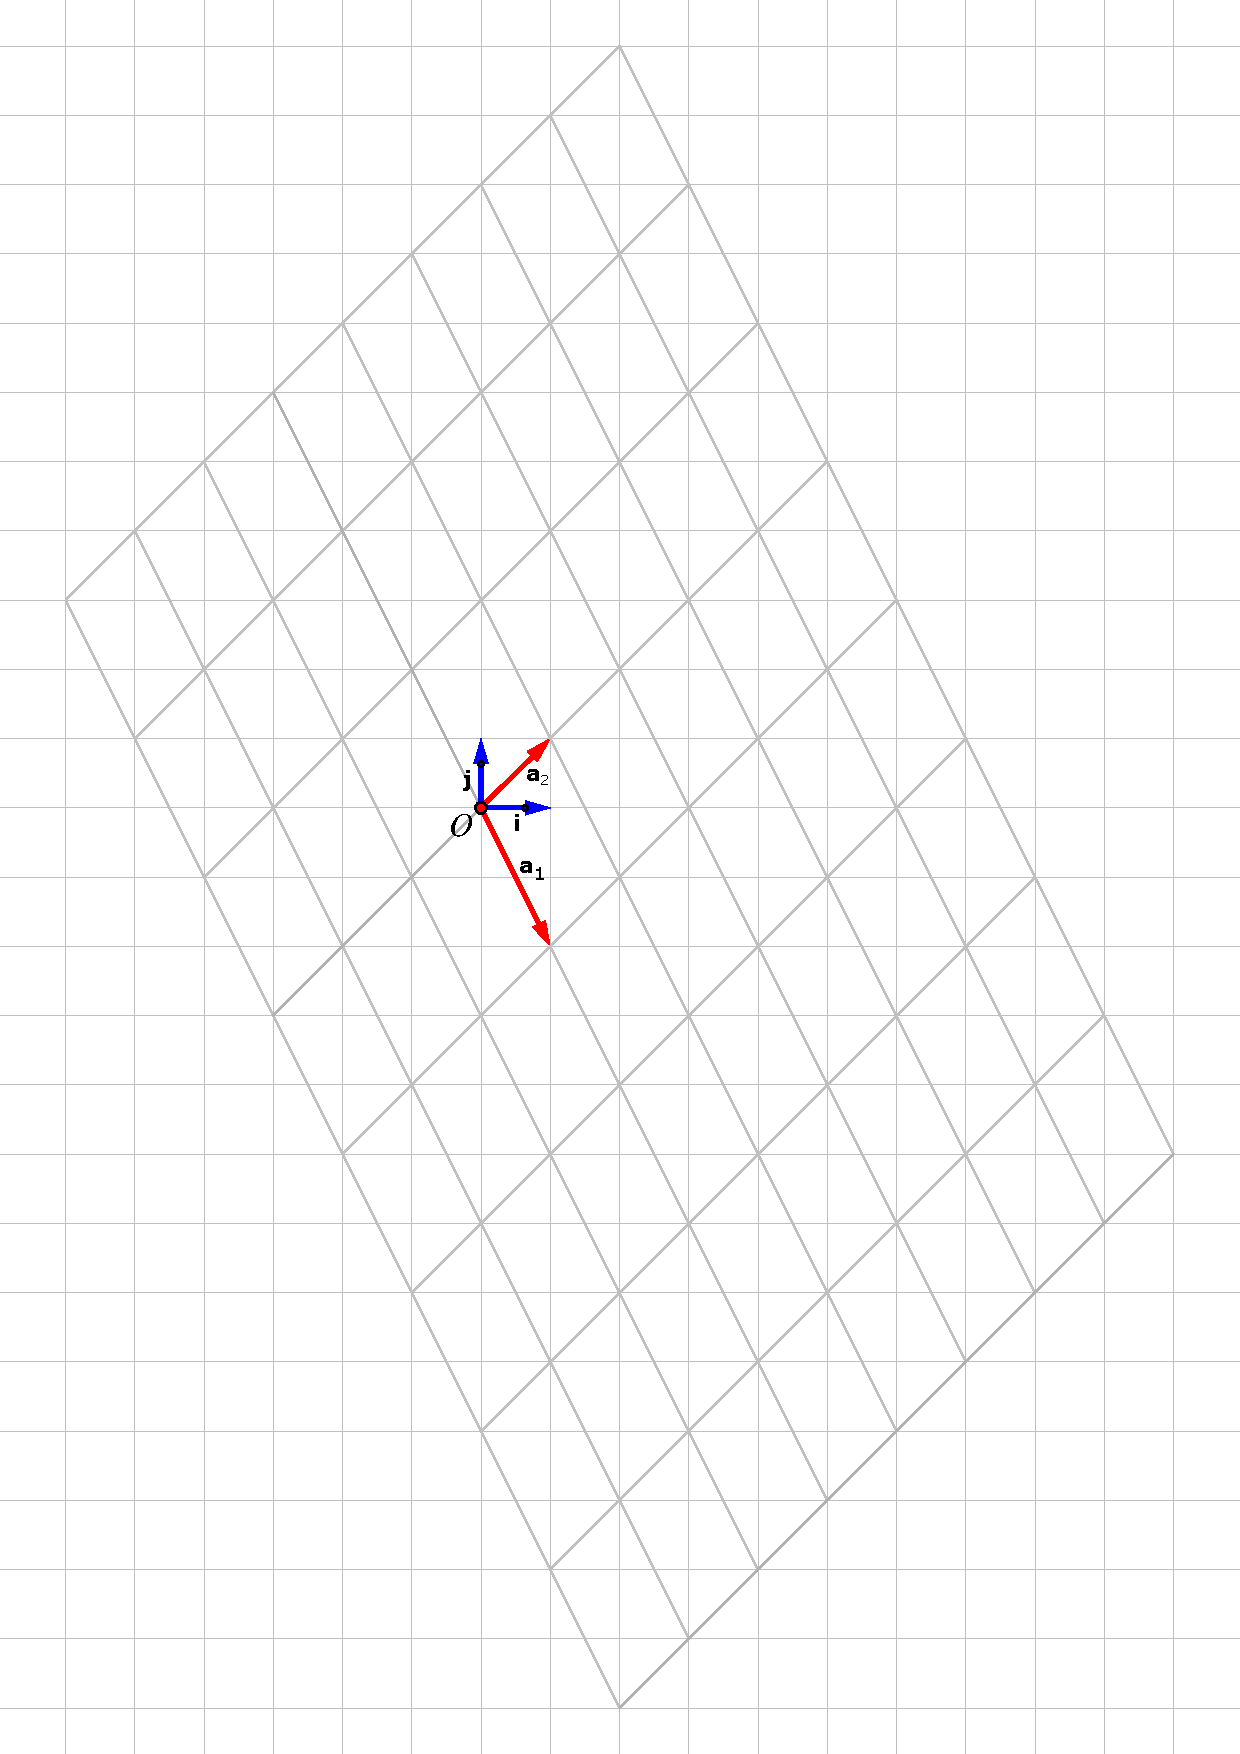
\includegraphics[trim=3cm 12.5cm 4.5cm 11cm,width=0.7\textwidth,clip]{geometer/abasis05.pdf}			
		\\Figur 6.27: Basisskifte
\end{center}
På figur 6.27 er der i planen givet standard e-basen $(\mathbf i, \mathbf j)$ samt en a-basis $(\mathbf a_1, \mathbf a_2)$. Når der skiftes basis, ændres givne vektorers koordinater. Her opstiller vi en systematisk metode til at udtrykke ændringen i koordinater ved hjælp af et matrixvektorprodukt. Først aflæser vi a-basisvektorernes e-koordinater:
\begin{equation}
{_\mathrm{e}\mathbf{a_1}}=\begin{matr}{r}1\\-2 \end{matr}\,\,\mathrm{og}\,\,\,{_\mathrm{e}\mathbf{a_2}}=\begin{matr}{r}1\\1 \end{matr}\,.
\end{equation}
\begin{enumerate}
\item
\textit{Opgave}: Antag at en vektor $\mv$ har koordinatsættet ${_\mathrm{a}\mathbf{v}}=\begin{matr}{r}v_1\\v_2 \end{matr}$\,. Bestem e-koordinaterne for $\mv$.\\

\textit{Løsning}: Vi har at $\mv=v_1\ma_1+v_2\ma_2$ og dermed i følge sætning \ref{tn6.koord_linearitet}:
$$ 
{_\mathrm{e}\mathbf{v}}=v_1\begin{matr}{r}1\\-2 \end{matr}
+v_2\begin{matr}{r}1\\1 \end{matr} = \begin{matr}{rr}1&1\\-2&1 \end{matr}\,
\begin{matr}{r}v_1\\v_2 \end{matr}
$$
Hvis vi sætter $\mM=\begin{matr}{rr} 1&1\\-2&1 \end{matr}$, udtrykkes $\mv$'s e-koordinater ved matrixvektorproduktet
\begin{equation}
{_\mathrm{e}\mathbf{v}}=\mM \cdot {_\mathrm{a}\mathbf{v}}\label{tn6.basisskifte3}
\end{equation}
\item
\textit{Opgave}: Antag at en vektor $\mathbf u$ har koordinatsættet ${_\mathrm{e}\mathbf{v}}=\begin{matr}{r}u_1\\u_2 \end{matr}$\,. Bestem a-koordinaterne for $\mathbf u$.\\

\textit{Løsning}: Vi ganger fra venstre på begge sider af \ref{tn6.basisskifte3} med den inverse matrix til $\mM$, og får udtrykt a-koordinaterne for $\mathbf u$ ved matrixvektorproduktet:
\begin{equation}
{_\mathrm{a}\mathbf{v}}=\mM^{-1}\cdot {_\mathrm{e}\mathbf{v}}\label{tn6.basisskifte4}
\end{equation}
\end{enumerate}
\end{example}
\begin{exercise}\label{tn6.koordmatrix4}
Ved en \ind{koordinatmatrix}{koordinatmatrix} med hensyn til en given basis a for et sæt af vektorer forstår man den matrix der opstår når man sætter vektorernes a-koordinatsøjler sammen til en matrix.\\
Beskriv matricen $\mathbf T$ i eksempel \ref{tn6.koordmatrix1} og \ref{tn6.koordmatrix2} og matricen $\mM$ i \ref{tn6.koordmatrix3} som koordinatmatricer. 
 
\end{exercise}
%%%%%%%%%%%%%%%%%%%%%%%%%%%%%%%%%%%%%%%%%%%%%%%%%%%%%%%%
%
%%%%%%%%%%%%%%%%%%%%%%%%%%%%%%%%%%%%%%%%%%%%%%%%%%%%%%%%%
\section{Sætninger om vektorer i en standard e-basis}
I dette afsnit arbejder vi med standard-koordinatsystemer, både i planen og rummet. Vi indfører to forskellige multiplikationer mellem vektorer, prikproduktet der både defineres i planen og rummet, og krydsproduktet der kun defineres i rummet. Vi ser på geometriske anvendelser af disse multiplikationsformer og på geometriske fortolkninger af determinanter.
\subsection{Prikproduktet af to vektorer}

\begin{definition}[Prikprodukt i planen]
I planen er der givet to vektorer
${_\mathrm{e}\mathbf{a}}=\begin{matr}{r}a_1\\a_2 \end{matr}\,$ og
${_\mathrm{e}\mathbf{b}}=\begin{matr}{r}b_1\\b_2 \end{matr}\,$. Ved \textit{prikproduktet} (eller \textit{skalarproduktet}) af $\ma$ og $\mb$  forstås tallet 
\begin{equation}
\ma \cdot \mb=a_1\cdot b_1+a_2\cdot b_2\,.
\end{equation}
\end{definition}

\begin{definition}[Prikprodukt i rummet]
I rummet er der givet to vektorer
${_\mathrm{e}\mathbf{a}}=\begin{matr}{r}a_1\\a_2\\a_3 \end{matr}\,$ og
${_\mathrm{e}\mathbf{b}}=\begin{matr}{r}b_1\\b_2\\b_3 \end{matr}\,$. Ved \textit{prikproduktet} (eller \textit{skalarproduktet}) af $\ma$ og $\mb$  forstås tallet 
\begin{equation}
\ma \cdot \mb=a_1\cdot b_1+a_2\cdot b_2+a_3\cdot b_3\,.
\end{equation}
\end{definition}

For prikproduktet mellem to vektorer gælder de følgende regneregler.\\

\begin{theorem}[Regneregler for prikprodukt]\label{prikregneregler}
Givet tre vektorer $\ma$, $\mb$ og $\mc$ i planen eller rummet samt tallet $k$. Der gælder:
\begin{enumerate}
\item
$\ma \cdot \mb = \mb \cdot \ma$ (kommutativ regel)
\item
$\ma \cdot (\mb+\mc)=\ma \cdot \mb + \ma \cdot \mc$ (associativ regel)
\item
$(k\ma) \cdot \mb=\ma \cdot (k\mb)=k(\ma \cdot \mb)$
\item
$\ma \cdot \ma = |\ma|^2$ 
\item
$|\ma+\mb|^2=|\ma|^2+|\mb|^2+2\ma \cdot \mb.$
\end{enumerate}
\end{theorem}

\begin{bevis}
Reglerne 1, 2, 3 følger af simpel koordinatudregning. Regel 4 følger af Pythagoras' sætning, og regel 5 er en direkte følge af reglerne 1, 2 og 4.
\end{bevis}
I de efterfølgende tre sætninger ser vi på geometriske anvendelser af prikproduktet.

\begin{theorem}[Længde af en vektor]
Lad $\mv$ være en vilkårlig vektor i planen eller rummet. Længden af $\mv$ opfylder
\begin{equation}
|\mv|=\sqrt{\mv \cdot \mv\,}\,.
\end{equation}
\end{theorem}
\begin{bevis}
Sætningen følger umiddelbart af regneregel 4 i \ref{prikregneregler}
\end{bevis}
\begin{example}[Længde af en vektor]
Givet vektoren $\mv$ i rummet og at ${_\mathrm{e}\mathbf{v}}=(1,2,3)$. Vi har da
$$
|\mv|=\sqrt{1^2+2^2+3^2}=\sqrt{14}\,.
$$
\end{example}
Den efterfølgende sætning handler om vinklen mellem to vektorer, se figur 6.28.
\begin{center}
		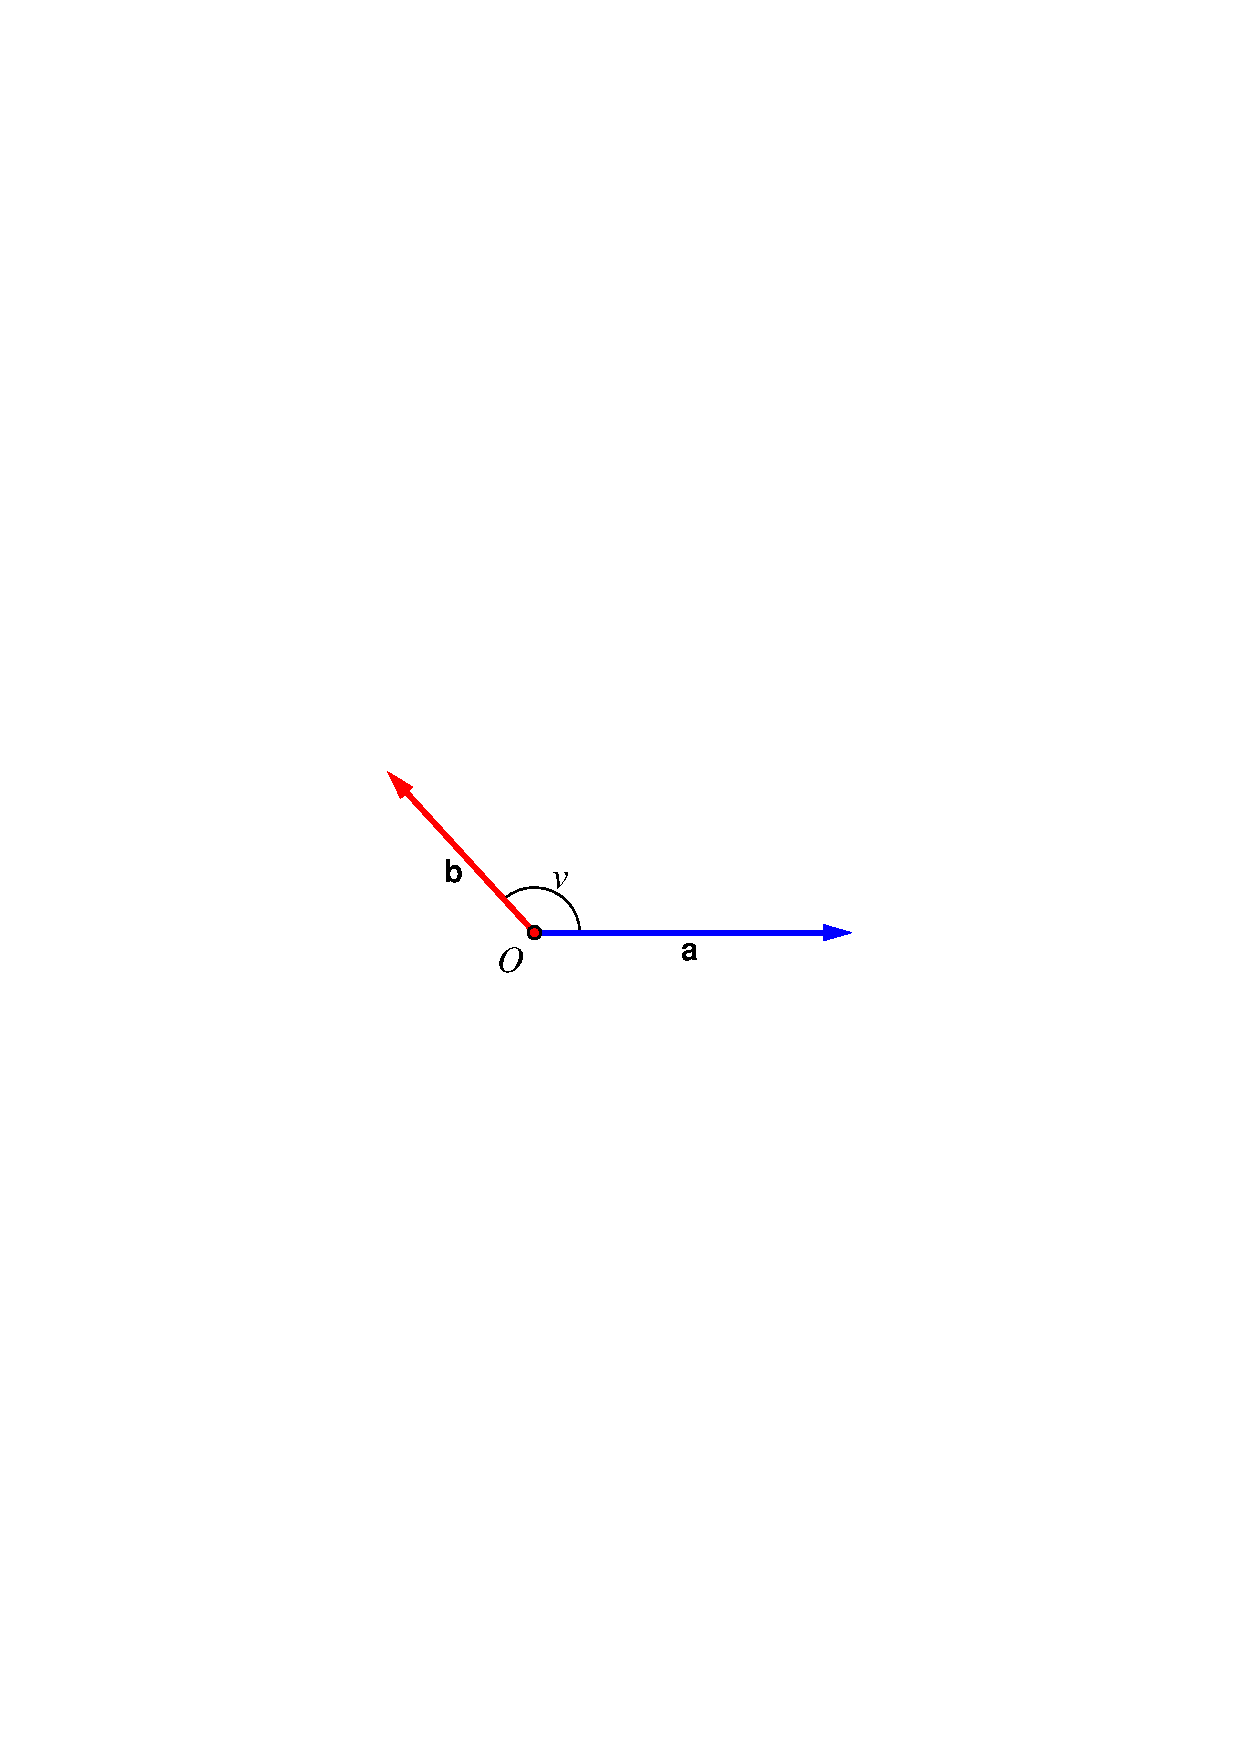
\includegraphics[trim=1.4cm 12.5cm 1.4cm 12cm,width=0.70\textwidth,clip]{geometer/skalarprod.pdf}	
		\\Figur 6.28
\end{center} 
\begin{theorem}[Vinkel mellem vektorer]\label{vinkel}
I planen eller rummet er der givet vektorerne $\ma$ og $\mb$. Vinklen v mellem $\ma$ og $\mb$ opfylder
\begin{equation}
\cos(v)=\frac{\ma \cdot \mb}{|\ma||\mb|}
\end{equation}
\end{theorem}

\begin{bevis}
Sætningen kan vises ud fra cosinus-relationen. Undervejs får man også brug for regel 5 i sætning \ref{prikregneregler}. Detaljerne overlades til læseren.
\end{bevis}
Af sætningen ovenfor følger umiddelbart denne sætning:

\begin{corollary}[Vinklers størrelsesforhold]
Betragt situationen i figur 6.28. Der gælder
\begin{enumerate}
\item
$\ma \cdot \mb=0\Leftrightarrow \mathrm{vinkel}(\ma,\mb)=\frac{\pi}{2}$
\item
$\ma \cdot \mb > 0\Leftrightarrow \mathrm{vinkel}(\ma,\mb)<\frac{\pi}{2}$
\item
$\ma \cdot \mb<0\Leftrightarrow \mathrm{vinkel}(\ma,\mb)>\frac{\pi}{2}$
\end{enumerate}
\end{corollary}

De to følgende sætninger er tilegnet \ind{ortogonal projektion}{ortogonale projektioner}. På figur 6.29 er der i planen eller rummet afsat to vektorer $\ma$ og $\mb$ ud fra origo.
\begin{center}
		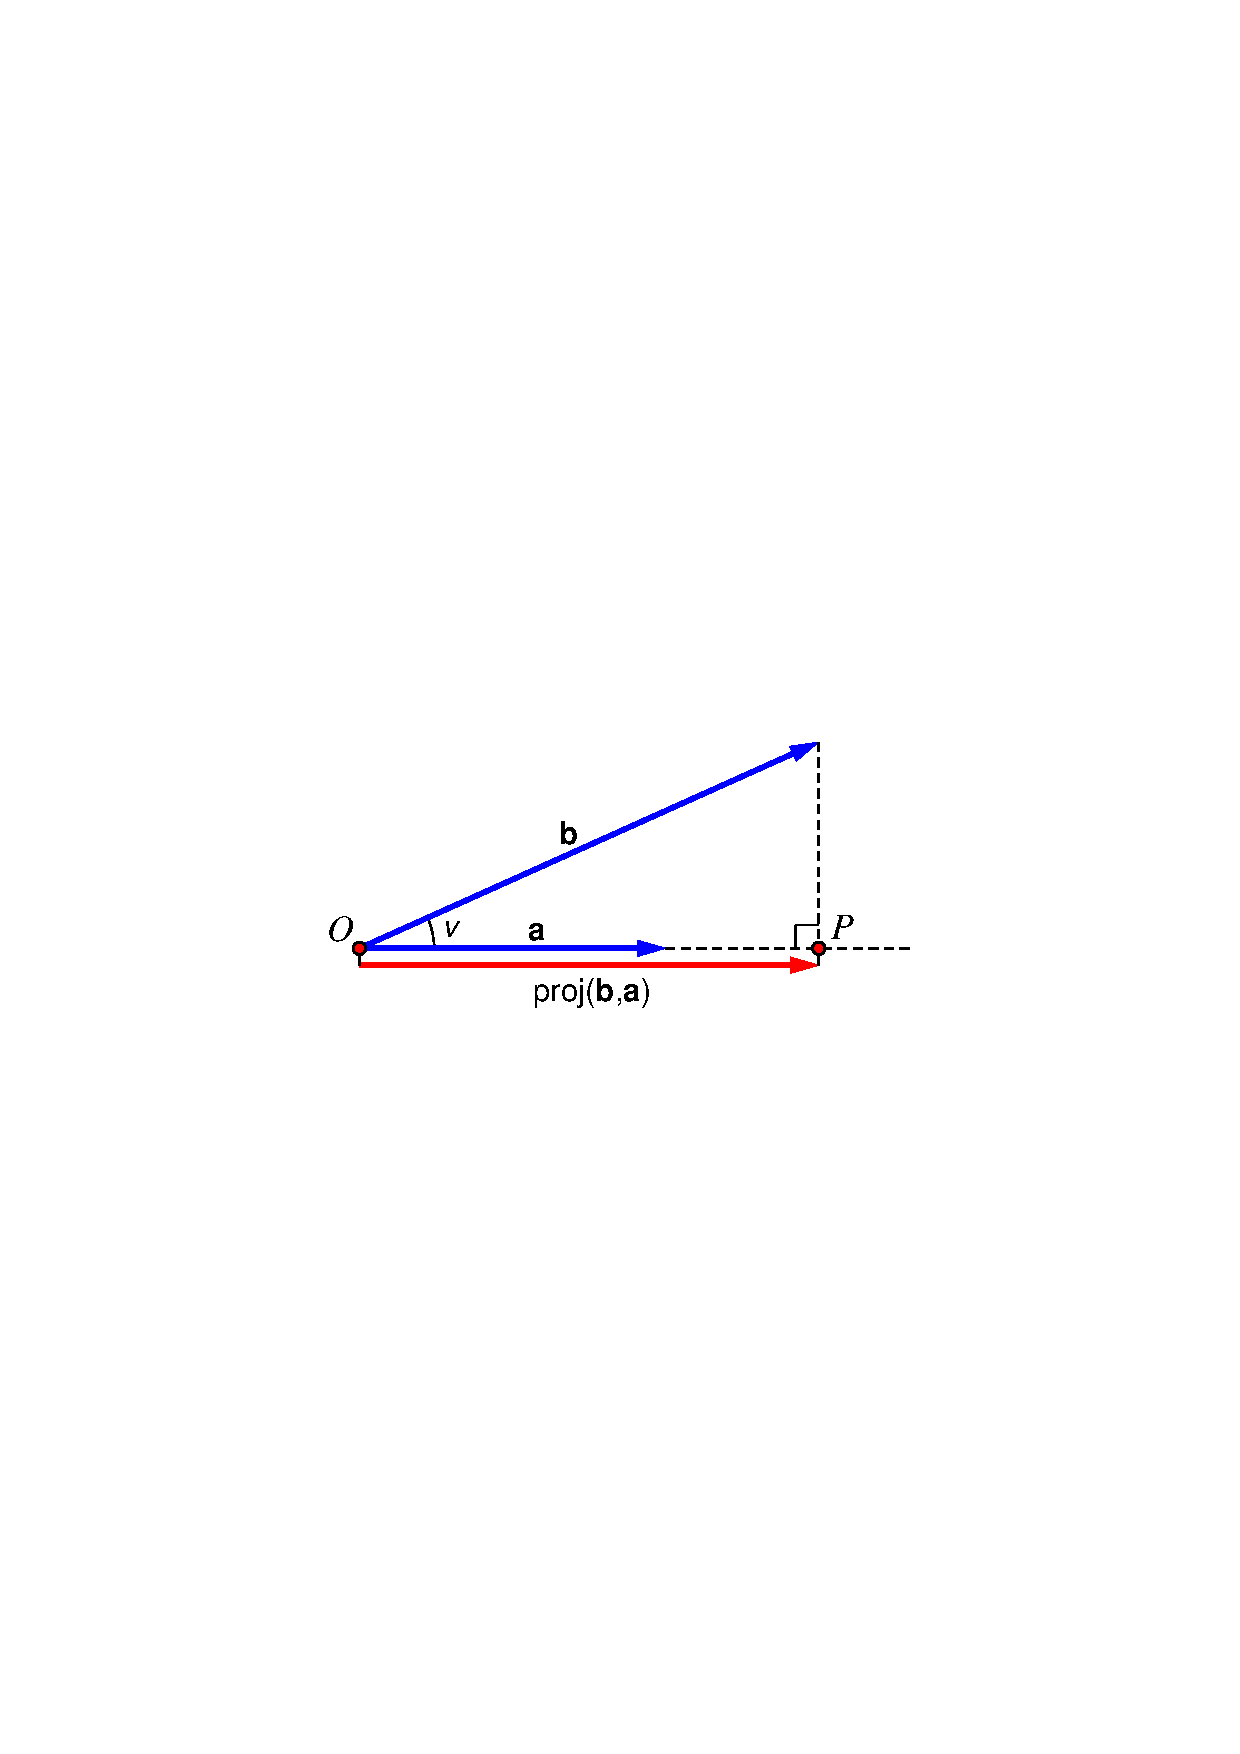
\includegraphics[trim=1.4cm 12cm 1.4cm 12cm,width=0.70\textwidth,clip]{geometer/proj.pdf}	
		\\Figur 6.29
\end{center} 
 Betragt det vinkelrette nedfældningspunkt $P$ af $\mb$'s endepunkt på den linje som indeholder $\ma$. Ved den ortogonale projektion af $\mb$ på $\ma$ forstås vektoren $\mathrm{proj}(\mb,\ma)=\stackrel{\rightarrow}{OP}$.
 
\begin{theorem}[Længen af en projektion]\label{projlength}
Givet to egentlige vektorer $\ma$ og $\mb$ i planen eller rummet. Om længden af den ortogonale projektion af $\mb$ på $\ma$ gælder: 
\begin{equation}
|\mathrm{proj}(\mb,\ma)|=\frac{|\ma \cdot \mb|}{|\ma|}
\end{equation}
\end{theorem}
\begin{bevis}
Ved brug af kendt sætning vedrørende retvinklede trekanter samt \ref{vinkel} fås
$$
|\mathrm{proj}(\mb,\ma)|=|\cos(v)|\,|\mb|=\frac{|\ma \cdot \mb|}{|\ma|}\,.
$$
\end{bevis}

\begin{theorem}[Formel for projektionsvektor]
Givet to egentlige vektorer $\ma$ og $\mb$ i planen eller rummet. Om den ortogonale projektion af $\mb$ på $\ma$ gælder: 
\begin{equation}
\mathrm{proj}(\mb,\ma)=\frac{\ma \cdot \mb}{|\ma|^2}\,\ma\,.
\end{equation}
\end{theorem}

\begin{bevis}
Hvis $\ma$ og $\mb$ er ortogonale er sætningen klart opfyldt da projektion da er nul-vektoren. I modsat fald, lad $sign(\ma \cdot \mb)$ betegne fortegnet for $\ma \cdot \mb$. Der gælder at $sign$ er positiv netop når $\ma$ og $\mathrm{proj}(\mb,\ma)$ er ensrettede og negativ netop når de er modsatrettede. Vi får derfor 
$$
\mathrm{proj}(\mb,\ma)=sign(\ma \cdot \mb)\cdot|\mathrm{proj}(\mb,\ma)|\,\frac{\ma}{|a|}=\frac{\ma \cdot \mb}{|\ma|^2}\,\ma\,,
$$
hvor vi undervejs har benyttet \ref{projlength}, og at $\frac{\ma}{|\ma|}$ er en enhedsvektor pegende i $\ma$'s retning.
\end{bevis}

\subsection{Geometrisk tolkning af determinant af $2\times 2$ matrix}
En trekant $\bigtriangleup = \bigtriangleup(p, \mathbf{a}, \mathbf{b})$ er bestemt ved to vektorer afsat ud fra et fælles begyndelelsespunkt, se trekant $\bigtriangleup = \bigtriangleup(p, \mathbf{a}, \mathbf{b})$, se figur 6.30.
\begin{center}
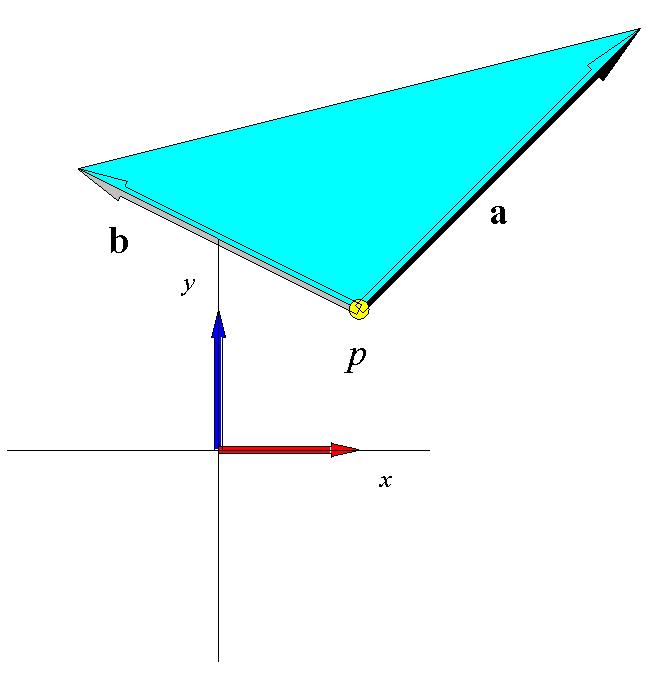
\includegraphics[height=70mm]{geometer/paborient.jpg}	
	\\Figur 6.30: En trekant udspændt af to vektorer i planen
\end{center}
Arealet af en trekant er som bekendt halvdelen af grundlinjen gange højden. Vi kan vælge længden $|\mathbf{a}|$ af $\mathbf{a}$ som grundlinje. Og højden i trekanten er
\begin{equation}
|\mathbf{b} | \sin(\theta) = \frac {|\mathbf{b} \cdot \widehat{\mathbf{a}}|} {| \widehat{\mathbf{a}}|}  \;,
\end{equation}
hvor $\theta$ er vinklen mellem de to vektorer $\mathbf{a}$ og $\mathbf{b}$, og hvor $\widehat{\mathbf{a}}$ betegner \ind{tværvektoren}{tværvektoren} i planen til $\mathbf{a}$, dvs. i koordinater har vi $\widehat{\mathbf{a}} = (-a_{2}, a_{1})$. Derfor er arealet:

\begin{equation} \label{tn6.eqAreaCalc}
\begin{aligned}
\Ar(\bigtriangleup(p, \mathbf{a}, \mathbf{b})) &= \frac{1}{2}|\mathbf{b} \cdot \widehat{\mathbf{a}}| \\
&= \frac{1}{2}|a_{1}b_{2} - a_{2}b_{1}| \\ &=
| \, \frac{1}{2}\left| \begin{array}{rr}
      a_{1} & b_{1} \\
      a_{2} & b_{2}
          \end{array}
 \right| \, | \\
&=  \frac{1}{2}|\,\det\left(\, \left[ \begin{array}{rr}
      a_{1} & b_{1} \\
      a_{2} & b_{2}
          \end{array} \right]\,\right)\, | \\
&=
\frac{1}{2}|\,\det\left(\, \left[ \mathbf{a}\,\,\mathbf{b} \right]\,\right)\, |\, \;.
\end{aligned}
\end{equation}

Vi har hermed vist sætningen:

\begin{theorem}[Areal af trekant ved determinant]
 Arealet af trekant $\bigtriangleup(p, \mathbf{a}, \mathbf{b})$ er den numeriske værdi af den halve determinant af den $2\times 2$ matrix, der fås ved at sætte $\mathbf{a}$ og $\mathbf{b}$ ind som søjler i matricen.\\
\end{theorem}

\subsection{Krydsprodukt og rumprodukt}

\textit{Krydsproduktet} af to vektorer og \textit{rumproduktet} af tre vektorer indføres ved hjælp af determinanter:
 
\begin{definition}[Krydsprodukt]
I rummet er der givet to vektorer
${_\mathrm{e}\mathbf{a}}=\begin{matr}{r}a_1\\a_2\\a_3 \end{matr}$ og
${_\mathrm{e}\mathbf{b}}=\begin{matr}{r}b_1\\b_2\\b_3 \end{matr}\,$.\\

Ved \textit{krydsproduktet} (eller \textit{vektorproduktet}) $\ma\times\mb$ af $\ma$ og $\mb$  forstås vektoren $\mv$ givet ved
\begin{equation}
{_\mathrm{e}\mathbf{v}}=\begin{matr}{r}
\det\,
\begin{matr}{rr}a_2 & b_2\\a_3 & b_3 \end{matr} 
\\
\det\,
\begin{matr}{rr}a_3 & b_3\\a_1 & b_1 \end{matr} 
\\
\det\,
\begin{matr}{rr}a_1 & b_1\\a_2 & b_2 \end{matr} 
\end{matr}
\end{equation}
\end{definition}

Krydsproduktet har en markant geometrisk betydning, sammenhold figur 6.31 og den efterfølgende sætning:
\begin{center}
		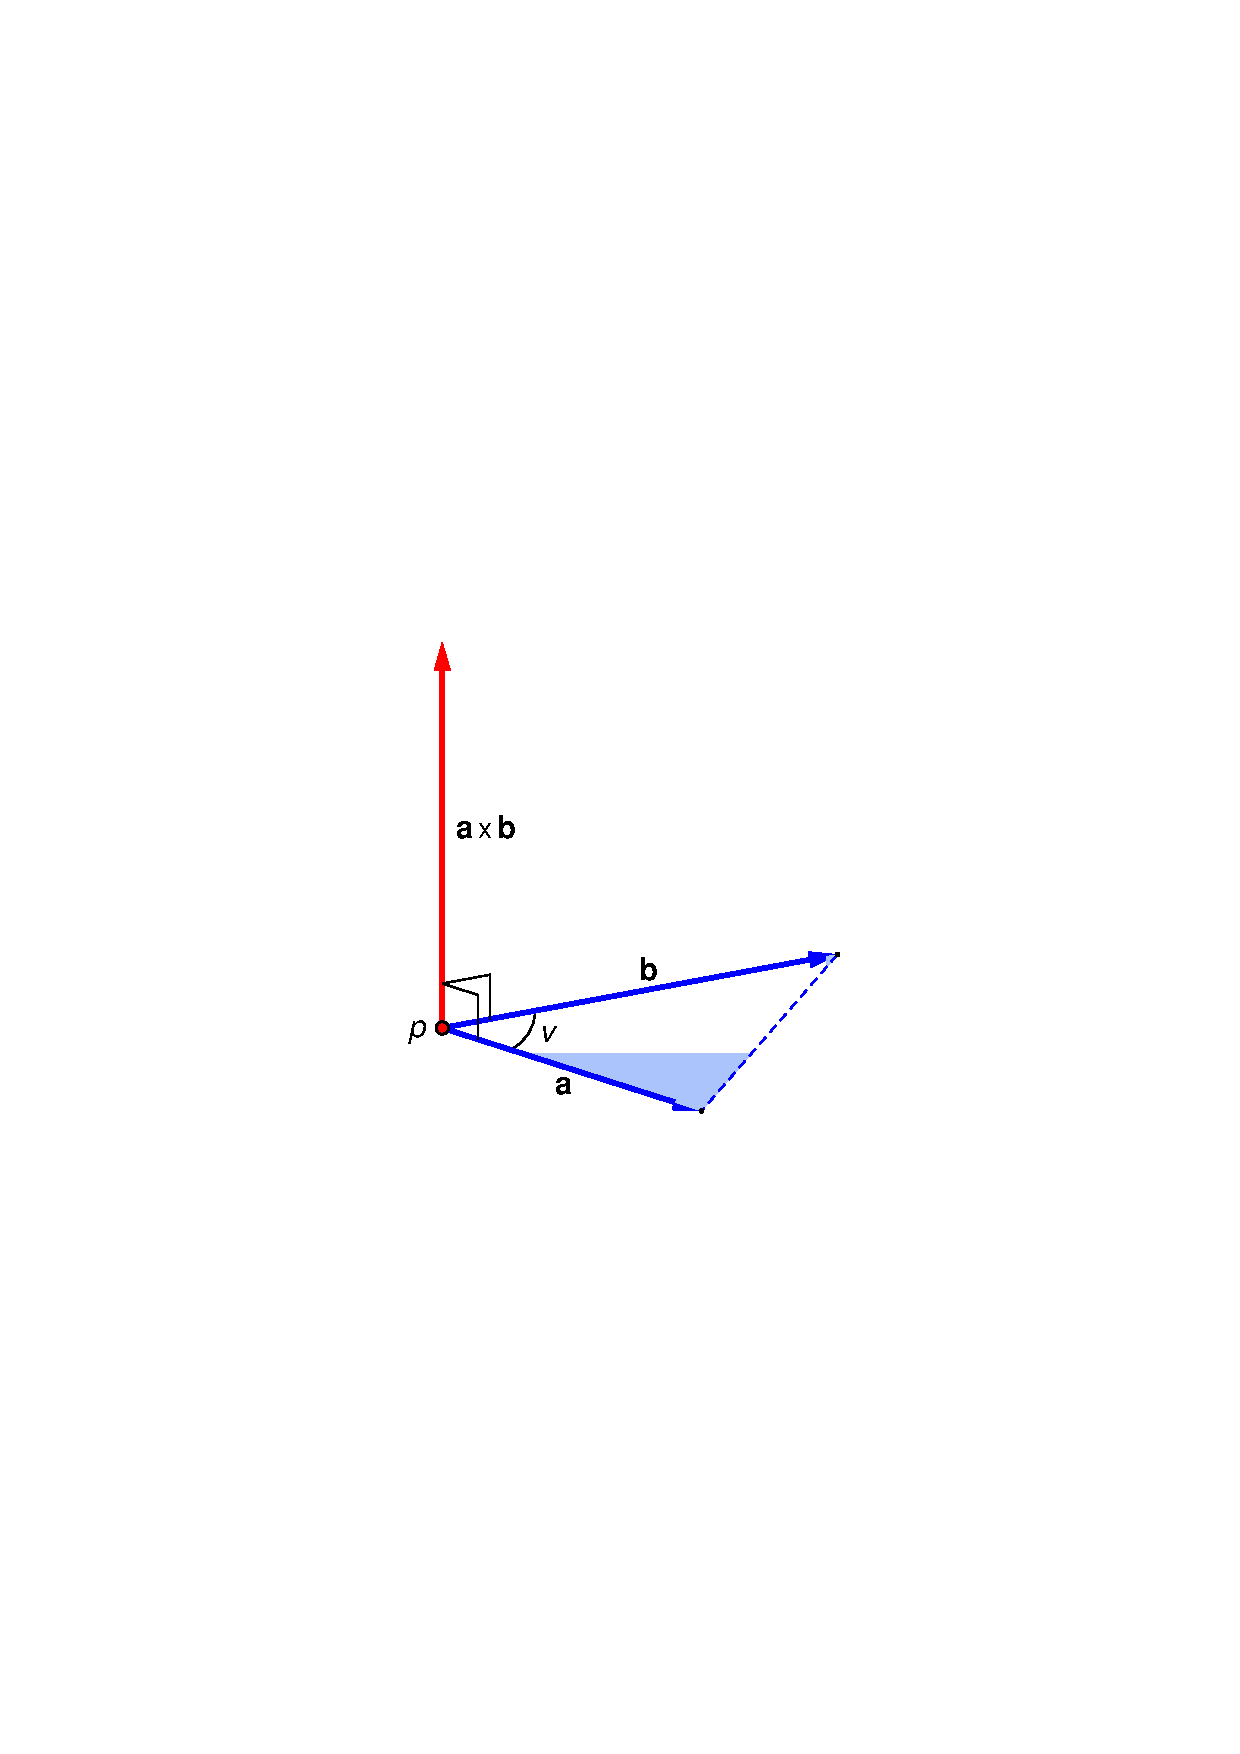
\includegraphics[trim=1.4cm 10.5cm 1.4cm 10.7cm,width=0.60\textwidth,clip]{geometer/krydsprodukt.pdf}	
		\\Figur 6.31
\end{center} 
\begin{theorem}[Areal af trekant ved krydsprodukt]\label{tn6.ArTrekant3d}
For to lineært uafhængige vektorer $\ma$ og $\mb$ som har den  mellemliggende vinkel $v$, opfylder krydsproduktet $\ma\times\mb$
\begin{enumerate}
\item
$\ma\times\mb$ er ortogonal på både $\ma$ og $\mb$\,.
\item
$|\ma\times\mb| = 2\cdot\Ar(\bigtriangleup(p, \mathbf{a}, \mathbf{b}))$
\,. 
\item
Vektorsættet $(\ma,\mb,\ma\times\mb)$ er i højrestilling.
\end{enumerate}
\end{theorem}

\begin{definition}[Rumprodukt]\label{rumprodukt}
 Rumproduktet $\Rum(\mathbf{a}, \mathbf{b}, \mathbf{c})$ af tre vektorer
 ${_\mathrm{e}\mathbf{a}}=\begin{matr}{r}a_1\\a_2\\a_3 \end{matr}\,$, 
 ${_\mathrm{e}\mathbf{b}}=\begin{matr}{r}b_1\\b_2\\b_3 \end{matr}\,$ og
 ${_\mathrm{e}\mathbf{c}}=\begin{matr}{r}c_1\\c_2\\a_3 \end{matr}$
defineres ved:
 \begin{equation} \label{tn6.eqRumProd}
 \begin{aligned}
 \Rum(\mathbf{a}, \mathbf{b}, \mathbf{c}) &= (\mathbf{a} \times \mathbf{b})\cdot \mathbf{c}\\
 &= (c_{1}(a_{2}b_{3}-a_{3}b_{2}) + c_{2}(a_{3}b_{1}-a_{1}b_{3})+ c_{3}( a_{1}b_{2}-a_{2}b_{1}) \\
 &= \det\left( \left[
                 \begin{array}{rrr}
                   a_{1} & b_{1} & c_{1} \\
                   a_{2} & b_{2} & c_{2} \\
                   a_{3} & b_{3} & c_{3} \\
                 \end{array}
               \right]
  \right) \\
  &= \det\left( \left[{_\mathrm{e}\mathbf{a}} \, {_\mathrm{e}\mathbf{b}} \, {_\mathrm{e}\mathbf{c}}
               \right]
  \right)\quad.
 \end{aligned}
 \end{equation}
 \end{definition}
 
\subsection{Geometrisk tolkning af determinant af $3\times 3$ matrix}
Fra elemtær rumgeometri vides at rumfanget af et tetraeder er en tredjedel af grundfladens areal gange højden. Betragt tetraederet 
$\boxtimes = \boxtimes(p,\mathbf{a}, \mathbf{b}, \mathbf{c})$ udspændt af vektorerne $\ma, \mb$ og $\mc$ afsat udfra punktet $p$, på figur 6.32.
\begin{center}
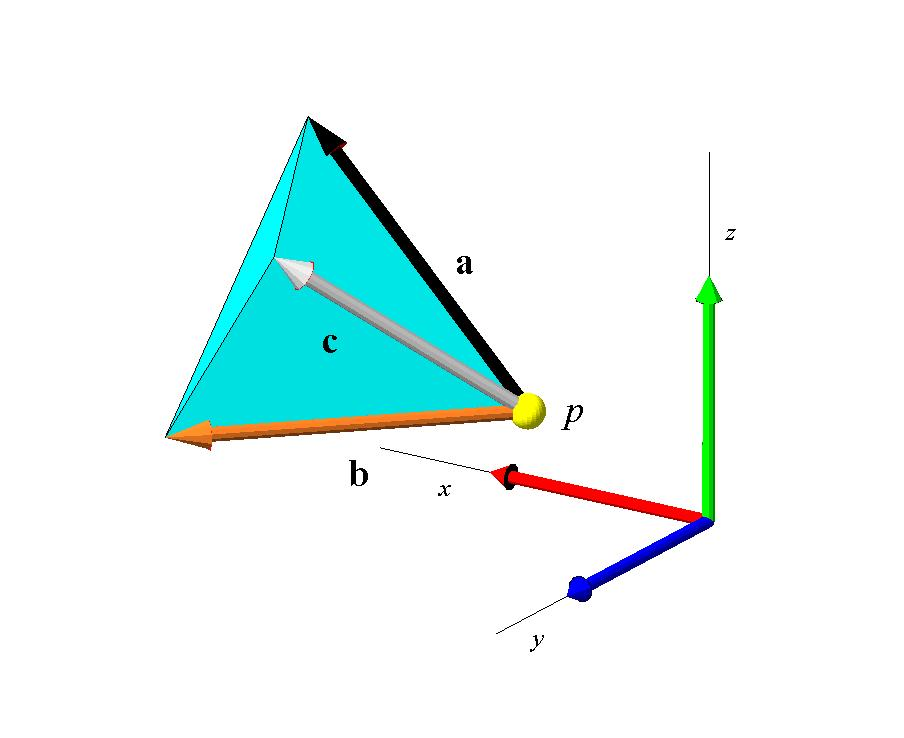
\includegraphics[height=70mm]{geometer/Tripod01.jpg}	
	\\Figur 6.32: Et tetraeder udspændt af tre vektorer i rummet
\end{center}

Arealet af grundfladen, $\bigtriangleup(p, \mathbf{a}, \mathbf{b})$ har vi bestemt i del 2 af sætning \ref{tn6.ArTrekant3d}.\\

Højden kan vi dernæst bestemme som skalarproduktet af den sidste kant-vektor $\mathbf{c}$ med en enhedsvektor, som står vinkelret på grundtrekanten.\\

Men $\mathbf{a} \times \mathbf{b}$ står netop vinkelret på grundtrekanten (fordi krydsproduktet er vinkelret på grundtrekantens kant-vektorer, se del 2 af sætning (\ref{tn6.ArTrekant3d}), så den kan vi bruge:
\begin{equation} \label{tn6.eqRumfang01}
\begin{aligned}
\Vol(\boxtimes(p,\mathbf{a}, \mathbf{b}, \mathbf{c})) &= | \frac{1}{3}\Ar(\bigtriangleup(p, \mathbf{a}, \mathbf{b}))\,\frac{(\mathbf{a} \times \mathbf{b})\cdot \mathbf{c}}{| \mathbf{a} \times \mathbf{b} |} | \\
&= \frac{1}{6}|(\mathbf{a} \times \mathbf{b})\cdot \mathbf{c}|
\end{aligned}
\end{equation}
hvor vi har benyttet del 2 af sætning \ref{tn6.ArTrekant3d}.\\

Ved at sammenholde dette med definition på \textit{rumprodukt}, se \ref{rumprodukt}, får vi nu rumfanget af et tetraeder skrevet kort på 'determinant-form':

\begin{theorem}[Rumfang af tetraeder ved rumprodukt]
Rumfanget af tetraederet $\boxtimes = \boxtimes(p,\mathbf{a}, \mathbf{b}, \mathbf{c})$ er:
\begin{equation} \label{tn6.eqVolDet}
\Vol(\boxtimes(p,\mathbf{a}, \mathbf{b}, \mathbf{c})) = \frac{1}{6}| \det\left( \left[\mathbf{a} \, \mathbf{b} \, \mathbf{c}
               \right]
  \right) | \quad.\\
\end{equation}
 \end{theorem}

Et tetraeder har rumfang $0$, er kollapset, netop når determinanten i (\ref{tn6.eqVolDet}) er $0$, og det forekommer præcist når en af vektorerne kan skrives som en linearkombination af de to andre (hvorfor det?).

\begin{definition}[Regulært tetraeder]
Et \ind{regulært tetraeder}{regulært tetraeder} er et tetraeder, der har et egentligt rumfang, altså et rumfang, der er skarpt større end $0$.
\end{definition}

\begin{exercise}
Lad $\mathbf{A}$ betegne en $(2 \times 2)$-matrix med søjlevektorerne $\mathbf{a}$ og $\mathbf{b}$:
\begin{equation}
\mathbf{A} = [\, \mathbf{a} \,\, \mathbf{b} \,] \quad.
\end{equation}
Vis, at determinanten af $\mathbf{A}$ er $0$ hvis og kun hvis søjle-vektorerne $\mathbf{a}$ og $\mathbf{b}$ er lineært afhængige i $\mathbb{R}^{2}$.
\end{exercise}

\begin{exercise}
Lad $\mathbf{A}$ betegne en $(3 \times 3)-$matrix med søjlevektorerne $\mathbf{a}$, $\mathbf{b}$, og $\mathbf{c}$:
\begin{equation}
\mathbf{A} = [\, \mathbf{a} \,\, \mathbf{b}\,\, \mathbf{c} \,] \quad.
\end{equation}
Vis, at determinanten af $\mathbf{A}$ er $0$ hvis og kun hvis søjle-vektorerne $\mathbf{a}$, $\mathbf{b}$ og  $\mathbf{c}$ udgør et lineært afhængigt system af vektorer i $\mathbb{R}^{3}$.
\end{exercise}

\begin{exercise}
Benyt de geometriske tolkninger af determinanten ovenfor til at vise, at der gælder følgende Hadamard's ulighed for $(2\times 2)-$matricer og for  $(3\times 3)-$matricer
(faktisk er uligheden rigtig for alle kvadratiske matricer):
\begin{equation} \label{tn6.eqHadamard}
(\det(\mathbf{A}))^{2} \leq \prod_{j}^{n}\left(\sum_{i}^{n}a_{ij}^{2}\right) \;.
\end{equation}
Hvornår gælder der lighedstegn i (\ref{tn6.eqHadamard})?
\end{exercise}

%%%%%%%%%%%%%%%%%%%%%%%%%%%%%%%%%%%%%%%%%%%%%%%%%%%%%%%%%%
%%%%%%%%%%%%%%%%%%%%%%%%%%%%%%%%%%%%%%%%%%%%%%%%%%%%%%%%%%
%%%%%%%%%%%%%%%%%%%%%%%%%%%%%%%%%%%%%%%%%%%%%%%%%%%%%%%%%%


\end{document} 


\end{document}  